% Basic Springer Nature Reference Style/Chemistry
% \documentclass[pdflatex,bst/sn-basic]{bst/sn-jnl}
% Style for submissions to Nature Portfolio journals
\documentclass[sn-nature]{bst/sn-jnl}
% Basic Springer Nature Reference Style/Chemistry
% \documentclass[bst/sn-basic]{bst/sn-jnl}
% Math and Physical Sciences Reference Style
% \documentclass[bst/sn-mathphys,Numbered]{bst/sn-jnl}
% American Physical Society (APS) Reference Style
% \documentclass[bst/sn-aps]{bst/sn-jnl}
% Vancouver Reference Style
%\documentclass[bst/sn-vancouver,Numbered]{bst/sn-jnl}
% APA Reference Style
% \documentclass[bst/sn-apa]{bst/sn-jnl}
% Chicago-based Humanities Reference Style
% \documentclass[bst/sn-chicago]{bst/sn-jnl}
% Default with double column layout
% \documentclass[default]{bst/sn-jnl}
% \documentclass[default]{bst/sn-jnl_mine}% Default
\jyear{2023}
%\usepackage{graphicx}
%\usepackage{multirow}
\usepackage{amsmath,amssymb,amsfonts}
%\usepackage{amsthm}
%\usepackage{mathrsfs}
%\usepackage[title]{appendix}
%\usepackage{xcolor}
%\usepackage{textcomp}
%\usepackage{manyfoot}
%\usepackage{algorithm}
%\usepackage{algorithmicx}
%\usepackage{algpseudocode}
%\usepackage{listings}
%\usepackage{setspace}
\usepackage{tabulary,fancyhdr,amsbsy,latexsym}
\usepackage{url,morefloats,floatflt,cancel,tfrupee}
\usepackage{colortbl}
\usepackage{pifont}
\usepackage[nointegrals]{wasysym}
\usepackage{float}
\usepackage{siunitx}
\usepackage{tabularx, booktabs}
\usepackage{lipsum}
\usepackage{fix-cm}
\newcommand{\figurepath}[1]{figures/#1}
\definecolor{mygreen}{HTML}{E9ECE6}
\usepackage{framed}
% \newenvironment{mymdframed}[1]{
% 	\begin{framed}
%         \textbf{#1} \par
%         }
%     {\end{framed}}

% \setlength{\parskip}{1.1em}% Adding space after each paragraph
\setlength{\parindent}{0pt}% Removing the indentation
\linespread{1.5}% Increase the line spacing to 1.5

\begin{document}

\title[Article Title]{Crowd-Certain: Label Aggregation in Crowdsourced and Ensemble Learning Classification}
\author[]{\fnm{Mohammad S.} \sur{Majdi}}
\author[]{\fnm{Jeffrey J.} \sur{Rodriguez}}
\affil[]{\orgdiv{Dept of Electrical and Computer Engineering}, \orgname{The University of Arizona}, \orgaddress{\city{Tucson}, \state{AZ}, \country{USA}}}

\abstract{
        Crowdsourcing systems have been used to accumulate massive amounts of labeled data for applications such as computer vision and natural language processing.
        However, because crowdsourced labeling is inherently dynamic and uncertain, developing a technique that can work in most situations is extremely challenging.
        In this paper, we introduce Crowd-Certain, a novel approach for label aggregation in crowdsourced and ensemble learning classification tasks that offers improved performance and computational efficiency for different numbers of annotators and a variety of datasets.
        The proposed method uses the consistency of the annotators versus a trained classifier to determine a reliability score for each annotator.
        Furthermore, Crowd-Certain leverages predicted probabilities, enabling the reuse of trained classifiers on future sample data, thereby eliminating the need for recurrent simulation processes inherent in existing methods.
        We extensively evaluated our approach against ten existing techniques across ten different datasets, each labeled by varying numbers of annotators.
        The findings demonstrate that Crowd-Certain outperforms the existing methods (Tao, Sheng, KOS, MACE, MajorityVote, MMSR, Wawa, Zero-Based Skill, GLAD, and Dawid Skene), in nearly all scenarios, delivering higher average accuracy, F1 scores, and AUC rates across all tested scenarios, irrespective of the number of annotators involved.
        Additionally, we explored the performance of different confidence score measurement techniques, Freq and Beta, using two evaluation metrics: Expected Calibration Error (ECE) and Brier Score Loss.
        Our results show that Crowd-Certain achieves a higher Brier Score, and lower ECE across the majority of the examined datasets, suggesting a higher accuracy of probabilistic predictions.
    }
\keywords{
    % Supervised learning, crowdsourcing, confidence score, soft weighted majority voting, label aggregation, annotator quality, error rate estimation, multi-class classification, ensemble learning, uncertainty measurement

    Supervised learning, crowdsourcing, confidence score, soft weighted majority voting, label aggregation, annotator quality, error rate estimation, multi-class classification, ensemble learning, uncertainty measurement
    }

\maketitle
% \section{Introduction}\label{sec:taxonomy.introduction}
Chest X-ray (CXR) is a prevalent radiological examination for diagnosing lung and heart disorders, constituting a significant share of ordered imaging studies. Fast and accurate detection of different thoracic diseases, such as pneumothorax, is crucial for optimal patient care~\cite{bellaviti_Increased_2016}. However, interpreting CXRs can be challenging due to similarities between different thoracic diseases, which may result in misinterpretation even by experienced radiologists~\cite{delrue_Difficulties_2011}. Consequently, devising an accurate system to identify and localize common thoracic diseases can aid radiologists in minimizing diagnostic errors~\cite{crisp_Global_2014,silverstein_Most_2016}.
Progress in natural language processing (NLP) has enabled the collection of extensive annotated datasets such as ChestX-ray8~\cite{wang_ChestXRay8_2017}, PADCHEST~\cite{bustos_Padchest_2020}, and CheXpert~\cite{irvin_CheXpert_2019}, allowing researchers to develop more efficient and robust supervised learning algorithms.
Convolutional neural networks (CNNs) exhibit potential for learning intricate relationships between image objects. However, their training necessitates vast amounts of labeled data, which can be both expensive and time-consuming to acquire. Despite these challenges, deep learning techniques have become increasingly popular in medical imaging, especially in radiology, due to their ability to perform complex tasks with minimal human intervention~\cite{jaderberg_Spatial_2015}.
The timely diagnosis and effective treatment of diseases depend on the fast and accurate detection of anomalies in medical images. Deep learning techniques have made substantial progress in the medical imaging domain, exhibiting impressive success across various applications~\cite{litjens_Survey_2017a,eshghali_Machine_2023}.  Although recent advances in deep learning have facilitated the creation of CAD systems capable of classifying and localizing prevalent thoracic diseases using CXR images, most of these techniques have concentrated on specific diseases~\cite{jaiswal_Identifying_2019,lakhani_Deep_2017,pasa_Efficient_2019,ausawalaithong_Automatic_2018}, leaving ample opportunities to investigate a unified deep learning framework that can efficiently detect a broad spectrum of common thoracic diseases. Further, conventional classification methods are primarily designed for single-label predictions and struggle with multi-label classification, which requires predicting multiple labels for each input sample. In multi-label classification, common methods like the One-vs-All (OVA) approach exhibit limitations, including high computational complexity and an inability to capture intricate label relationships~\cite{tsoumakas_MultiLabel_2007}.

This paper aims to tackle the challenges of multi-label classification by introducing a hierarchical framework that incorporates the relationships between different classes to provide a more accurate classification framework. We propose one approach termed as ``loss-based'' for scenarios where ground truth is available, in which the proposed technique is applied to the loss function of a network (e.g., a classification or segmentation network such as DenseNet121~\cite{huang_Densely_2017} or U-Net~\cite{ronneberger_UNet_2015}). For scenarios where ground truth is not available, we propose an alternative approach termed as ``logit-based'', where the hierarchical framework is applied to the logit values of an existing pre-trained network. Logits are the output of the last layer of a neural network before applying the activation function. For multi-class problems with $K$ classes, the number of logits is $K$, and the value of each logit represents the model's confidence in the $k$-th class being positive. For example, consider a binary classification problem where one needs to determine if an email is spam. In that case, the logit will be a single value representing the confidence that the email is spam. The higher the value of the logit, the more confident the model is that the email is spam.
The logit-based technique provides a transfer learning approach that improves classification accuracy without necessitating an extensive computational investment. The rest of this paper is structured as follows. Section~\ref{sec:taxonomy.relatedwork} discusses related work on multi-label classification and hierarchical loss functions; Section~\ref{sec:taxonomy.methods} describes the proposed techniques for integrating label hierarchy into multi-label classification techniques; Section~\ref{sec:taxonomy.results} presents experimental results using the chest radiograph dataset; and Section~\ref{sec:taxonomy.discussion} concludes the paper and outlines future research directions.

\section{Related Work}\label{sec:taxonomy.relatedwork}
The introduction of the ChestX-ray8 dataset and its associated model~\cite{wang_ChestXRay8_2017} marked a significant advancement in large-scale CXR classification, leading to numerous improvements in both modeling and dataset collection. These enhancements include the integration of ensemble methods~\cite{islam_Abnormality_2017}, attention mechanisms~\cite{guan_Diagnose_2018,liu_SDFN_2019}, and localization techniques~\cite{cai_Iterative_2018,guendel_MultiTask_2019,li_Thoracic_2018,yan_Weakly_2018}. Most early approaches use ``binary relevance'' (BR) learning, which reduces the multi-label classification problem to binary classification by training a binary classifier for each class~\cite{zhang_Review_2014}. However, BR-based techniques do not account for label dependence---either conditional (instance-specific label dependence) where in a given instance the presence or absence of one label may impact another, or marginal (dataset-specific label dependence) where certain labels may co-occur more frequently~\cite{dembczynski_Label_2012}.
\\
Multi-label classification, unlike multi-class methods, classifies instances into multiple categories simultaneously. For example, a single chest radiograph image can have both edema and cardiomegaly~\cite{harvey_Standardised_2019,tsoumakas_MultiLabel_2007}. Significant research on integrating taxonomies through hierarchical classification was conducted prior to the advent of deep learning by extracting a set of binary hierarchical multi-label classification (HMLC) labels from pseudo-probability predictions~\cite{bi_BayesOptimal_2015}. Early methods used hierarchical and multi-label generalizations of traditional algorithms, such as nearest-neighbor or multi-layer perceptron~\cite{pourghassem_ContentBased_2008} and decision trees~\cite{dimitrovski_Hierarchical_2011}. With the rise of deep learning, the adaptation of convolutional neural networks (CNN) for hierarchical classification has gained increasing attention~\cite{guo_CNNRNN_2018,kowsari_HDLTex_2017,redmon_YOLO9000_2017,roy_TreeCNN_2020}.
\\
\textit{Hierarchical Multi-Label Classification Technique: }
In many cases, the diagnosis or observation of a particular condition on a CXR (or other medical imaging data) is dependent on the presence or absence of the parent class~\cite{vaneeden_Relationship_2012}. For example, if a radiologist is trying to diagnose pneumonia in a patient, they may first look for evidence of lung consolidation (parent label) in the CXR\@. Consequently, it is possible to make more accurate diagnoses by taking into account the relationship between labels\@. However, many existing CXR classification methods do not consider the dependence between labels and instead treat each label independently. These algorithms are known as ``flat classification'' methods~\cite{alaydie_Exploiting_2012}. Furthermore, some labels at the lower levels of the hierarchy, specifically leaf nodes, have very few positive examples, making the flat learning model susceptible to negative class bias. To address these issues, we must create a model that considers the hierarchical nature of the CXR\@.
\\
Hierarchical multi-label classification methods have been successfully implemented in a variety of domains, including text processing~\cite{aly_Hierarchical_2019}, visual recognition~\cite{bi_Mandatory_2014}, and genomic analysis~\cite{bi_BayesOptimal_2015}. A common technique~\cite{chen_Deep_2019} for exploiting such a hierarchy is to train a classifier on conditional data while ignoring all samples with negative parent-level labels and then reintroducing these samples to fine-tune the network across the entire dataset~\cite{chen_Deep_2019}. These approaches help the classifier focus on the relevant data during initial training, thus improving the prediction accuracy.  However, these techniques are computationally expensive, as they require training a classifier on conditional data and then fine-tuning it on a full dataset. This makes them difficult to apply to real-world problems, where the amount of data is often very large.   Another common strategy is a cascading architecture where different classifiers are trained at each level of the hierarchy. Although these techniques enable more granular data analysis (each classifier can focus on a specific level of the hierarchy), they require a substantial amount of computational resources. Other existing deep learning-based approaches often use complex combinations of CNNs and recurrent neural networks (RNNs)~\cite{guo_CNNRNN_2018,kowsari_HDLTex_2017}.

\section{Methods}\label{sec:taxonomy.methods}
In this study, we introduce a unique method that improves the accuracy and interpretability of multi-label classification, with potential applications in areas such as chest radiography. We propose two distinct strategies. The first strategy termed as ``loss-based'', requiring the availability of ground truth labels, incorporates the hierarchical relationships among different classes directly into the loss function. In contrast, the second strategy termed as ``logit-based'' utilizes these hierarchical relationships to modify the logit values before calculating the predicted probabilities for each class. These two strategies, which utilize a transfer learning approach, foster the use and fine-tuning of pre-existing models, thereby expanding their adaptability to new tasks. By improving the accuracy of classifying different pathologies, these techniques could potentially enhance disease diagnosis and treatment.
The proposed technique is adaptable to the available computational resources. When ample computational resources are available, the ``loss-based'' strategy can be utilized. Alternatively, in scenarios with limited computational resources, to avoid the need for optimization of the network from scratch, the ``logit-based'' strategy can be utilized.
One notable advantage of our proposed techniques lies in enhancing interpretability. By categorizing classes into a hierarchical structure and capitalizing on their relationships, the model not only improves classification performance but also provides insights into the relationships among predicted classes.
This additional layer of interpretability can help radiologists in understanding the reasoning behind the model's predictions, fostering trust in the model's output and facilitate its integration into clinical workflows. Furthermore, the hierarchical nature of the taxonomy allows radiologists to explore predictions at various levels of granularity, depending on the level of detail required for a specific case.
%
\subsection{Problem Formulation}\label{subsec:taxonomy.problem_formulation}
\subsubsection{Mathematical Formulation of Sigmoid Function}
In the context of neural networks, a logit refers to the raw, unscaled output of a neuron. This output is obtained at the last layer of a neural network model prior to the application of the sigmoid layer~\cite{furnieles_Sigmoid_2022}. Logit values can range from negative to positive infinity. The term ``logit'' originally comes from logistic regression, and it is the inverse of the logistic sigmoid function. In machine learning, it's often desirable for our model to produce real numbers ranging from 0 to 1. Applying the sigmoid function to the logit ensures this, as the sigmoid function maps any real number to the interval \([0,1]\).
The equation representing the sigmoid function is:
\begin{equation}
p = \text{{sigmoid}}(q) = \frac{1}{1 + e^{-q}}
\end{equation}
When we apply this sigmoid function to the logit values produced by the neural network, the result is a predicted probability ranging from 0 to 1. This property is particularly useful in binary classification tasks, where the aim is to model the probability of a given input pertaining to a certain class.
In a binary classification scenarios, if we apply the sigmoid function to the logit value and obtain output \( p \), we interpret this as the model's estimated probability that the input belongs to the class.
Finally, the equation for the logit (also known as the log-odds) can be given as
\begin{equation}
q = \text{{logit}}(p) = \log \left( \frac{p}{1 - p} \right)
\end{equation}
where \( p \) is the probability of a positive event. This function maps a probability \( p \) from the interval \((0,1)\) to any real number.
%
\subsubsection{Glossary of Symbols}\label{subsubsec:notations}
Let us define the following parameters:
\begin{itemize}
    \item  $\mathcal{C} = {\{c_k\}}_{k=1}^{K}  $: the set of classes (categories) in the multi-label dataset, where $c_k $ is the name of the $k $-th class.
    \item  $\mathcal{E} $: set of edges representing parent-child relationships between classes.
    \item  $\mathcal{G}=\left\{\mathcal{C},\mathcal{E}\right\} $:  Graph representing the taxonomy of thoracic diseases.
    \item  $c_j=\Lambda (c_k) \in \mathcal{C}$: parent class of class $c_k $ in graph $\mathcal{G} $.
    \item  $\mathcal{J}(c_j) \subset \mathcal{C}$: set of child classes of class $c_j$ in graph $\mathcal{G} $
    \item  $y_k^{(i)} \in \{0,1\} $: true label for the $k $-th class of instance $i $.
    \item  $q_k^{(i)} \in \left( -\infty,0 \right) $: logits obtained in the last layer of the neural network model before the sigmoid layer.
    \item  $p_k^{(i)} = \text{sigmoid}\left(q_k^{(i)}\right) = \frac{1}{1+\exp{\left(-q_k^{(i)}\right)}} $: predicted probability for the $k $-th class ($c_k) $ of instance $i $ with a value between 0 and 1. $p_k^{(i)} $ represents the likelihood that class $k $ is present in instance $i $ and is obtained by passing logits $q_k^{(i)} $ through a sigmoid function.
    \item  $\theta_k $: Binarization threshold for class $k $.  To obtain this, we can utilize any existing thresholding technique (for example, in one technique, we analyze the ROC curve and find the corresponding threshold where the difference between the true positive rate (sensitivity) and false positive rate (1-specificity) is maximum; alternatively, we could simply use $0.5 $).
    \item  $t_k^{(i)}=\left\{\begin{array}{ll}1&\text{if}\;p_k^{(i)} \geq \theta_k\\0&\text{otherwise.}\end{array}\right. $: predicted label obtained by binarizing the $p_k^{(i)} $
    \item  ${\widehat p}_k^{(i)} \in (0,1) $: updated predicted probability for the $k $-th class of instance $i $ with a value between 0 and 1.
    \item  $\widehat{t}_k^{(i)}=\left\{\begin{array}{ll}1&\text{if}\;\widehat{p}_k^{(i)}\geq\theta_k\\0&\text{otherwise.}\end{array}\right. $: updated predicted label for the $k $-th class of instance $i $.
    \item $K $: number of categories (aka classes) in a multi-class, multi-label problem. For example, suppose that we have a dataset that is labeled for the presence of cats, dogs, and rabbits in any given image. If a given image $X^{(i)} $ has cats and dogs but not rabbits, then $Y^{(i)} = \{1,1,0\} $.
    \item $N $: Number of instances.
    \item $X^{(i)} $: Data for instance $i$.
    \item $Y^{(i)}=\left\{y_1^{(i)},y_2^{(i)},\;\dots,y_{K}^{(i)}\right\} $: True label set for instance $i $. For example, consider a dataset that is labeled for the presence of cats, dogs, and rabbits in any given instance. If a given instance $X^{(i)} $ has cats and dogs but not rabbits, then $Y^{(i)}=\{1,1,0\} $.
    \item $P^{(i)} = {\left\{ p_k^{(i)} \right\}}_{k=1}^{K} $: Predicted probability set obtained in the output of the classifier $F(\cdot) $ representing the probability that each class $k $ is present in the sample.
    \item $T^{(i)} = {\left\{t_k^{(i)}\right\}}_{k=1}^{K} $: predicted label set for instance $i $.
    \item $\mathbb{X} = {\left\{X^{(i)}\right\}}_{i=1}^{N} $: Set of all instances.
    \item $\mathbb{Y} = {\left\{Y^{(i)}\right\}}_{i=1}^{N} $: Set of all true labels.
    \item $\mathbb{D}=\left\{\mathbb{X},\mathbb{Y}\right\} $: Dataset containing all instances and all true labels.
    % \item  $\mathbb{D}_{\text{phase1}},\mathbb{D}_{\text{phase2}} $: randomly selected subsets of the $\mathbb{D} $ dataset used for phase1: training the machine learning model and phase2: applying the proposed taxonomy technique. $\mathbb{D}_{\text{phase1}}\cup\;\mathbb{D}_{\text{phase2}}=\mathbb{D} $ and $\mathbb{D}_{\text{phase1}} \bigcap \mathbb{D}_{\text{phase2}} = \varnothing $
    \item $l_k^{(i)} = \mathcal{L} \left(y_k^{(i)},p_k^{(i)}\right) $:  $\mathcal{L}(\cdot)$ is an arbitrary loss function (e.g., binary cross entropy) that takes the true label $y_k^{(i)}$ and predicted probability $p_k^{(i)}$ for class $k$ and instance $i$ and outputs the loss value $l_k^{(i)} $. We refer to this as the ``base loss function'' throughout this paper.
    \item $\text{Loss}(\theta) $: Measured loss for all classes and instances. This value is obtained using a modified version of the base loss function $\mathcal{L}(\cdot) $ (e.g., with added regularization, etc.).
    \item $\omega_k^{(i)} $: Estimated weight for $k$-th class $c_k $ of instance $i $ with respect to its parent class $\Gamma_k $.
    \item ${\widehat l}_k^{(i)} = \omega_k^{(i)} \; l_k^{(i)} $: updated loss for class $k $ and instance $i $.
    % \item  ${\widehat p}_k^{(i)}=\omega_k^{(i)}\;p_k^{(i)} $: updated predicted probability for the $k $ -th class.
\end{itemize}
%
Let us define the multi-label classification problem as follows. Let $\mathbb{X} = {\left\{X^{(i)}\right\}}_{i=1}^{N} $ be a set of $N $ chest radiograph images and $\mathbb{Y} = {\left\{Y^{(i)}\right\}}_{i=1}^{N} $ be their corresponding ground truth labels. The ground-truth labels for the dataset were provided by experienced radiologists who annotated each image with the corresponding abnormalities.

Given the set of disease classes $\mathcal{C} = \{c_1,c_2,\dots,c_K\} $, let us define a  graph $\mathcal{G}=\left\{\mathcal{C},\mathcal{E}\right\} $ representing the taxonomy of thoracic diseases, where $\mathcal{E}$ is the set of edges representing parent-child relationships between these classes. For each node $c_k \in \mathcal{C} $, let $\Lambda (c_k)$ be the parent node of class $c_k $ and let $\mathcal{J}_k\subset \mathcal{C} $ be the set of child classes of class $c_k $ in graph $\mathcal{G}$. \\
In the context of multi-label classification problems, each sample may have multiple labels assigned to it simultaneously. To this end, we use a deep neural network, with multiple hidden layers and the sigmoid activation function in the final layer. Let's denote the input to this neural network by $x^{(i)}$, which represents data for instance $i$ (data type can be a 1D feature vector, 2D image, or 3D volume). This network is trained to predict the probabilities for each class being present in a given sample. Hence, the output of the final layer of the neural network for instance $i$ is passed through a sigmoid function to generate a set of values, each ranging from 0 to 1, corresponding to the label set $\mathcal{C} $.
The outcome of this operation is a set of $K $ predicted probabilities $P^{(i)}={\left\{p_k^{(i)}\right\}}_{k=1}^{K} $. Each of these predicted probabilities, derived from the sigmoid activation function, can be interpreted as the likelihood that the input sample belongs to each class.

Furthermore, let $\omega_k^{(i)} $ be a scalar weight assigned to the class $c_k $ of instance $i $ with respect to its parent class $\Lambda (c_k)$.
Each of these predicted probabilities, derived from the sigmoid activation function, can be interpreted as the likelihood that the input sample belongs to each class. A loss function is utilized to quantify the similarity between predicted probabilities and true labels. This function guides the learning process of the neural network by providing a measure of the prediction error, which is minimized during the training phase.
Let us denote the loss value as $l_k = \mathcal{L} \left(p_k^{(i)},y_k^{(i)}\right),\hspace{0.33em}k \in \{1,2,\dots,K\} $ where $\mathcal{L}(\cdot) $ is an appropriate single-class loss function for the task (e.g., binary cross-entropy, Dice, etc.) that is used to calculate the difference between the predicted probability $p_k^{(i)} $ and the true class label $y_k^{(i)} $ for instance $i$ and class $k $.

\subsection{Label Taxonomy Structure}\label{subsec:label-taxonomy-and-hierarchy}
To exploit the hierarchical relationships between thoracic abnormalities, the first step is to define a disease taxonomy that demonstrates different abnormalities' interrelationships. In this taxonomy, diseases are structured hierarchically in a graph, with higher levels representing broader disease categories and lower levels representing more nuanced distinctions between related diseases. The taxonomy is structured such that if a disease is present then its parent disease is also present. Furthermore, in the presence of multiple parent classes for a given child class, the taxonomy structure only utilizes the more dominant parent (e.g., if class $c_1$ has two parent classes $c_3$ and $c_5$, while the $c_5$ is also the parent of $c_3$ class (it's both the parent and grandparent of $c_1$ class), in this scenario, we assume $c_5$ as the parent class of both $c_1$ and $c_3$).
%
For example, pleural effusion and pneumothorax can be classified as subcategories of pleural abnormalities, whereas atelectasis and consolidation can be classified under pulmonary opacity~\cite{irvin_CheXpert_2019}. This hierarchical structure enables the model to take advantage of the relationships between diseases to improve its classification performance.
In medical imaging, classes are frequently organized as graphs to represent the hierarchical relationships between different classes. For example, a graph can be used to represent the human body's organs, with each node representing a different organ and the edges representing the relationships between organs (e.g., the liver is part of the abdominal cavity). Using a graph structure for labels in medical imaging has a number of advantages, including improved accuracy and interpretability of classification algorithms, which are essential for making sense of the vast amounts of data generated by medical imaging technologies. In medical imaging, hierarchies of labels are typically constructed by subject matter experts with a comprehensive understanding of human anatomy and physiology, such as radiologists.
%
To create the label taxonomy shown in Figure~\ref{fig:taxonomy.fig.1.taxonomy_structure}, we combined the taxonomies provided by Irvin~\cite{irvin_CheXpert_2019} for the CheXpert dataset, Chen~\cite{chen_Deep_2020} for the PADCHEST~\cite{bustos_Padchest_2020} and the CXR portion of the prostate, lung, colorectal and ovarian (PLCO) dataset~\cite{gohagan_Prostate_2000}.
In order to maintain uniformity, we adopted the renaming scheme introduced by Cohen~\cite{cohen_TorchXRayVision_2022} for the pathology names. Subsequently, the key pathologies were identified and extracted to build the hierarchical taxonomy structure illustrated in Figure~\ref{fig:taxonomy.fig.1.taxonomy_structure}.
%

\subsection{Approach 1: Conditional Predicted Probability}\label{subsec:taxonomy.method.approach1}
When computational resources are limited, this technique can be applied to test samples without the need to fine-tune the pre-trained, multi-label classification model. This adaptability ensures that the benefits of considering hierarchical relationships between labels can be realized in a wide range of practical scenarios, without imposing excessive computational requirements.
Directly updating the predicted probabilities presents potential benefits, including the following:
\begin{itemize}
    \item  \textbf{Simplicity:} Direct modification of predicted probabilities eliminates the need for substantial changes to the loss function, thus facilitating implementation.
    \item  \textbf{Improved performance in specific scenarios:} Depending on the problem and dataset, direct updates may provide superior performance in certain circumstances, especially when incorporating class relationships into the loss function is challenging.
    \item  \textbf{Easier calibration:} Direct modification of predicted probabilities can facilitate calibration of the model output to more closely match the true label distribution.
\end{itemize}
The proposed technique provides an easy way to improve the performance of existing pre-trained models during inference time by updating the value of the predicted logit for each class that was obtained at the last layer of the neural network based on the predicted logit of its corresponding parent class. The aim is to calculate the conditional predicted probability for each class $k $ and instance $i $, taking into account the predicted probability of the parent class. We can formalize this by defining a new predicted probability for the $k$-th class $(c_k) $ and instance $i $ as follows.
\begin{equation}
    \widehat{p}_k^{(i)} = \frac{1}{ 1 + \exp \left(-\left(q_k^{(i)} + \alpha_k q_j^{(i)} \right)\right) }
    \label{eq:taxonomy.eq.1.pred.approach1}
\end{equation}
where $c_j = \Lambda (c_k)$ is the index of the parent class of the $k$-th class, and $\alpha_k $ is the hyperparameter that controls the influence of different parent class logits on child class logits.
When $\alpha_k=0 $, there is no influence from the parent class $c_j$ on the child class $c_k$.  By carefully selecting appropriate hyperparameter values, this transfer learning technique can be employed to effectively adjust the predicted probabilities of each class, considering the hierarchical relationship between classes, and potentially improving classification accuracy.

\subsubsection{Parameter Selection and Tuning}
The selection of appropriate hyperparameters is crucial for the effectiveness of the proposed transfer learning technique. In this study, we employ a systematic approach to tune the hyperparameter vector $\{\alpha_k \}_{k=1}^K$ , which controls the dependency between the predicted probabilities of the child and parent classes. We utilize a grid search method to determine the optimal values for these hyperparameters. The search space for the hyperparameters is defined based on preliminary experiments and domain knowledge, ensuring a balance between model complexity and predictive performance.

The steps are as follows.
\begin{enumerate}
    \item Pre-process the data. Details shown in Algorithm~\ref{alg:taxonomy.dataset}
    \item Get logit values. Details shown in Algorithm~\ref{alg:taxonomy.logits}
    \begin{itemize}
        \item Fine Tune $f_1(\cdot)$, using $\mathbb{D}^{\text{train}}$ and $\mathbb{D}^{\text{valid}}$.
        \item Create a secondary model $f_2 (\cdot)$ identical to $f_1(\cdot)$ except for the last activation layer (sigmoid). Update the weights and biases in the $f_2 (\cdot)$ using their counterparts in $f_1(\cdot)$
        \item Calculate the logit values
    \end{itemize}
    \item Perform Hyper Parameter Tuning to find the $\{\alpha_k \}_{k=1}^K$ values. The detail shown in Algorithm~\ref{alg:taxonomy.logit.hyperparameter-optimization}
    \begin{itemize}
        \item Determining the instances of $\alpha_k$ where the Area Under the Curve (AUC) calculated for the instances in train dataset is maximized.
        \item Optimization Algorithm: Tree-structured Parzen Estimator (TPE). TPE is a Sequential Model-Based Optimization (SMBO) method. It builds a hierarchical model of the hyperparameter space to suggest new hyperparameters, making it more efficient than grid and random search, in exploring large, high-dimensional spaces. TPE enhances efficiency by focusing on promising areas of the parameter space, guided by data from previous evaluations.
        \item Use the optimal hyperparameter vector $\{\alpha_k \}_{k=1}^K$ calculated in Algorithm~\ref{alg:taxonomy.logit.hyperparameter-optimization}, logit values in $\mathbb{T}^{\text{test}}=\left\{ \mathbb{Y}^{\text{test}}, \mathbb{Q}^{\text{test}} \right\}$, and Eq.~\ref{eq:taxonomy.eq.1.pred.approach1} to calculate the new predicted probabilities for test instances.
    \end{itemize}
\end{enumerate}

\begin{SgAlgorithm}
    \caption{Combining and Preprocessing Chest X-ray Datasets}\label{alg:taxonomy.dataset}
    \KwIn{
        \begin{itemize}
            \item $\mathbb{D}_{\text{NIH}} \gets \text{NIH dataset}$
            \item $\mathbb{D}_{\text{Chexpert}} \gets \text{CheXpert dataset}$
            \item $\mathbb{D}_{\text{PADCHEST}} \gets \text{PADCHEST dataset}$
        \end{itemize}
    }
    \BlankLine%

    \SetKwProg{Fn}{Data Preprocessing}{:}{end}
    \Fn{}
    {%
        \For{$\mathbb{X} \in \{ \mathbb{X}_\text{NIH}, \mathbb{X}_\text{Chexpert}, \mathbb{X}_\text{PADCHEST} \}$}
        {%
            Resize all images $x^{(i)} \in \mathbb{X}$ the resolution of $224 \times 224$ pixels. \;
            \BlankLine%

            Normalize the pixel intensities to the range of 0 and 1
        }
        \KwRet{$ \{ \mathbb{X}_\text{NIH}^{*}, \mathbb{X}_\text{Chexpert}^{*}, \mathbb{X}_\text{PADCHEST}^{*} \} $}
    }
    \BlankLine%

    \SetKwProg{Fn}{Updating Labels}{:}{end}
    \Fn{}
    {%
        \For{$\mathbb{Y} \in \{ \mathbb{Y}_\text{NIH}, \mathbb{Y}_\text{Chexpert}, \mathbb{Y}_\text{PADCHEST} \}$}
        {%
            Standardize labels (pathology names) to common schema \;
            \BlankLine%

            Extract 18 common pathologies:
            \begin{itemize}
                \item Atelectasis, Consolidation, Infiltration, Pneumothorax, Edema, Emphysema, Fibrosis, Effusion, Pneumonia, Pleural Thickening, Cardiomegaly, Nodule, Mass, Hernia, Lung Lesion, Fracture, Lung Opacity, Enlarged Cardiomediastinum
            \end{itemize}
        }
        \KwRet{$ \{ \mathbb{Y}_\text{NIH}^{*}, \mathbb{Y}_\text{Chexpert}^{*}, \mathbb{Y}_\text{PADCHEST}^{*} \} $}
    }
    \BlankLine%

    \SetKwProg{Fn}{Getting the Dataset}{:}{end}
    \Fn{}
    {%
        Combine datasets: $\mathbb{D} = \{ \mathbb{X}_{\text{NIH}}^{*}, \mathbb{Y}_{\text{NIH}}^{*} \}
        \cup
        \{ \mathbb{X}_{\text{Chexpert}}^{*}, \mathbb{Y}_{\text{Chexpert}}^{*} \}
        \cup
        \{ \mathbb{X}_{\text{PADCHEST}}^{*}, \mathbb{Y}_{\text{PADCHEST}}^{*} \}$
        \BlankLine%

        Split $\mathbb{D}$ into 3 subsets: $\mathbb{D}^\text{train}, \mathbb{D}^\text{valid}, \mathbb{D}^\text{test}$, representing 60\%, 10\%, and 30\% of data respectively
    }
    \BlankLine%
    \KwRet{$\mathbb{D}^\text{train}, \mathbb{D}^\text{valid}, \mathbb{D}^\text{test}$}
\end{SgAlgorithm}

\begin{SgAlgorithm}
    \caption{Computing Original Logit Values}\label{alg:taxonomy.logits}
    \KwIn{
        \begin{itemize}
            \item $\mathbb{D}^{\text{train}}, \mathbb{D}^{\text{valid}}, \mathbb{D}^{\text{test}}$ from Algorithm~\ref{alg:taxonomy.dataset}
            \item Baseline model architecture: DenseNet121, $f_1(\cdot)$
        \end{itemize}
    }
    \BlankLine%

    \SetKwProg{Fn}{Predictor Model}{:}{end}
    \Fn{$f_2(\cdot)$}
    {%
        Optimize model $f_1(\cdot)$ on $\mathbb{D}^{\text{train}}$ and $\mathbb{D}^{\text{valid}}$ \;

        Clone architecture of $f_1(\cdot)$ into $f_2(\cdot)$, without the last sigmoid activation. \;

        Update weights of $f_2(\cdot)$ from $f_1(\cdot)$
    }
    \BlankLine%

    \SetKwProg{Fn}{Calculating Logits}{:}{end}
    \Fn{$\text{getLogit}(\cdot)$}
    {%
        \KwIn{$\mathbb{D} = \left\{ \mathbb{X}, \mathbb{Y} \right\}, f_2(\cdot)$}
        \ForEach{$x^{(i)} \in \mathbb{X}$}
        {
            Compute logit vector ${\left\{ q_k^{(i)} \right\}}_{k=1}^K = f_2 \left(x^{(i)}\right)$
        }
        \BlankLine%
        ${\mathbb{Q}} = {\left\{ {\left\{ q_k^{(i)} \right\}}_{k=1}^K \right\}}_{i=1}^N$

        \KwRet{
            $\mathbb{T} = \left\{ \mathbb{Y}, \mathbb{Q} \right\}$
        }
    }
    \BlankLine%

    \textbf{Create New Dataset} \;
    ${\mathbb{T}}^\text{train} = \text{getLogit}(\mathbb{D}^\text{train})$ \;

    $\mathbb{T}^\text{test} = \text{getLogit}(\mathbb{D}^\text{test})$ \;
    \BlankLine%

    \KwRet{
        $\mathbb{T}^\text{train} , \mathbb{T}^\text{test}$
        }

\end{SgAlgorithm}

\begin{SgAlgorithm}
    \SetAlgoLined
    \caption{Hyper Parameter Optimization for Logit-Base Technique}\label{alg:taxonomy.logit.hyperparameter-optimization}
    \KwIn{%
        \begin{itemize}
            \item \textbf{Data} $\mathbb{T}^\text{train} = \left\{ \mathbb{Y}^\text{train} , \mathbb{Q}^\text{train} \right\} $
            \item \textbf{Number of iterations:} MAX\_EVALS
            \item \textbf{Search Space:} $ \mathcal{S} = \text{Uniform}(-1, 1) $
            \item \textbf{Predictor model $f_1(\cdot)$} that is trained on $\mathbb{D}^\text{train} = \left\{ \mathbb{X}^\text{train} , \mathbb{Y}^\text{train} \right\} $.
        \end{itemize}
    }
    \BlankLine%
    \SetKwProg{Fn}{ObjectiveFunction}{:}{end}
    \Fn{$\mathcal{O}$}
    {%
        \KwIn{$k, \alpha_k, \mathbb{Q}^\text{train}, \mathbb{Y}^\text{train}$}
        $ j \gets (c_j = \Lambda(c_k)) $ \;
        \ForEach{ $i, k$ }
        {
            $ \widehat{p}_k^{(i)} = \frac{1}{ 1 + \exp \left(-\left(q_k^{(i)} + \alpha_k q_j^{(i)} \right)\right) } $ (Eq.~\ref{eq:taxonomy.eq.1.pred.approach1})
        }
        \KwRet{ $ 1 - \text{AUC} \left( {\left\{ \widehat{p}_k^{(i)} \right\}}_{i=1}^N, {\left\{ y_k^{(i)} \right\}}_{i=1}^N \right) $ }
    }
    \BlankLine%
    \SetKwProg{Fn}{EstimatorFunction}{:}{end}
    \Fn{TPE}
    {%
        \KwIn{$\alpha_k^0, \mathcal{S}, \text{MAX\_EVALS}, k, \mathbb{Q}^\text{train}, \mathbb{Y}^\text{train}, \mathcal{O}(\cdot) $}
        \dots Tree-structured Parzen Estimator (TPE) \dots \;
        \KwRet{ $ \alpha_k^* $ }
    }
    \BlankLine%

    \textit{Optimization:} \;
    \For{ $k=1$ \KwTo~$K$}
    {%
        $ \alpha_k = 0 $ \;
        \If{$ \Lambda(c_k) \neq \varnothing $}
        {%
            $ \alpha_k =$ TPE($\alpha_k$, $\mathcal{S}$, $\mathcal{O}(\dots)$, MAX\_EVALS)
        }
    }
    \BlankLine%

    \KwRet{Optimal hyperparameters $ {\{ \alpha_{k} \}}_{k=1}^K $ }
\end{SgAlgorithm}

\subsection{Approach 2: Conditional Loss}\label{subsec:taxonomy.method.approach2}
In a second approach, we propose a similar concept to the approach discussed in Section~\ref{subsec:taxonomy.method.approach1}; however, rather than directly updating the predicted probability of each class, we instead update the loss value of each class based on the loss values of its parent classes. The utilization of the loss function approach can prove advantageous in certain scenarios, particularly in the context of multi-label classification tasks that involve hierarchical relationships, as it offers numerous benefits:
\begin{itemize}
    \item \textbf{Emphasis on error minimization:} The loss values quantify the divergence between the predictions made by the model and the actual labels provided as ground truth. Integrating parent class loss values into child class loss calculations aims to minimize errors throughout the hierarchy, with the goal of improving prediction accuracy for both parent and child classes.
    \item \textbf{Enhanced gradient propagation:} During the training process of deep learning models, the model parameters are updated by backpropagating gradients through layers. Incorporating the loss values of the parent class through the calculation of the loss for the child classes can improve the gradient propagation between the parent and child classes. This may lead to more effective learning of hierarchical associations and speed up the training convergence.
    \item \textbf{Robustness to label noise:} Real-world datasets may exhibit inconsistencies or noise in their ground truth labels. The inclusion of loss values from parent classes in the computation of loss values for child classes can enhance the consistency of the hierarchy by penalizing deviations from expected parent-child associations. This approach can result in improvement in the model's resilience to potential label inaccuracies in the dataset.
    \item \textbf{Improved interpretability:} The use of loss values rather than predicted probabilities enables a more straightforward understanding of the model's ability to capture hierarchical relationships among classes. When parent classes have high loss values, these losses influence their corresponding child classes' losses, underscoring the importance of improving the underlying model architecture and parameters to better present these hierarchical associations.
\end{itemize}

\subsubsection{Formulation of the Proposed Technique}
In multi-label classification problems, where each sample may belong to multiple classes, it is often necessary to combine the loss values for all classes to effectively train the model. Various methods can be employed to achieve this, depending on the specific problem. A common approach is to calculate the average loss across all classes for each sample by summing the losses for each class of a given sample and dividing the sum by the total number of classes to which the sample belongs. This method is effective when all classes are independent, of equal importance, and warrant equal weight in the total loss calculation. For example, in the case of cross-entropy loss, we have
\begin{equation}
    l_k \textcolor{gray}{\; = \; \mathcal{L} \left(y_k^{(i)},p_k^{(i)}\right)} \; = \; -\left(y_k^{(i)}\log(p_k^{(i)}) + (1 - y_k^{(i)})\log(1 - p_k^{(i)})\right)
    \label{eq:taxonomy.eq.2.loss}
\end{equation}
\begin{equation}
    \text{Loss}(\theta) = \sum_{i=1}^{N}\sum_{k=1}^{K}l_k
    \label{eq:taxonomy.eq.3.totalloss}
\end{equation}
In this formulation, the objective is to minimize the loss function with respect to the model parameters $\theta $, resulting in an optimal set of parameters that produce accurate predictions for multi-label classification tasks. However, class independence and equal importance between different classes cannot always be assumed. Inclusion of a hierarchical penalty or regularization term in the loss function is one way to push the loss function to take the taxonomy into account when optimizing the model hyperparameters (weights and biases).

Let's denote $\beta_k$ as the regularization term that penalizes the loss for class $c_k$ for each instance $i $ in which there is a low probability that it also belongs to parent class $c_j$. This can be represented mathematically by adding a hierarchical penalty term $H(c_k \vert c_j)$ for the class $c_k$ with respect to its corresponding parent class $c_j$ as follows:
\begin{equation}
    \widehat{l}_{k}^{(i)} = l_{k}^{(i)}+\beta_k H \left(c_k \vert c_j \right)
    \label{eq:taxonomy.eq.3.newloss}
\end{equation}
where $c_j=\Lambda(c_k)$, and $\beta_k $ is the hyperparameter that balances the contributions of class $k$'s own loss value and its parent class's loss values.
There are multiple ways to define the hierarchical penalty. For example, we can define it as the loss value of the parent class $l_j=\mathcal{L} \left(y_j^{(i)},p_j^{(i)}\right) $ as follows:
\begin{equation}
    H(k \vert j)=\mathcal{L} \left(y_j^{(i)},p_j^{(i)}\right)
    \label{eq:taxonomy.eq.4.hierarchical_penalty1}
\end{equation}
Another approach to incorporating the interdependence between different classes into the loss function is to apply the loss function $\mathcal{L} $ to the true label of the parent class and the predicted probability of the child class as follows.
\begin{equation}
    H(k\vert j)  = \mathcal{L} \left(y_j^{(i)},p_k^{(i)}\right)
    \label{eq:taxonomy.eq.5.hierarchical_penalty2}
\end{equation}
The penalization term in Equations~(\ref{eq:taxonomy.eq.4.hierarchical_penalty1}) and~(\ref{eq:taxonomy.eq.5.hierarchical_penalty2}) encourages the model to correctly predict the corresponding parent class when predicting the child class, hence ensuring that the predicted labels  align well with the hierarchical structure. The aforementioned approach, assumes a linear relationship  between the child and parent losses. However, this may not always accurately capture the relationship between the parent-child classes, as the relationship may not necessarily be linear.
The approach of multiplying losses introduces a greater adaptability in the representation of relationships between parent and child classes, as it can encapsulate both linear and potentially complex interrelations. Under the constraints of our problem -- where the absence of a parent class guarantees the absence of its child class -- both parent and child loss values would simultaneously increase or decrease (if the parent class is absent). In such a scenario, their summation or product would correspondingly escalate or diminish, thus demonstrating a linear relationship.
However, the complexity arises when we consider the scenario where the parent's loss value is significantly low in comparison to the child's loss. Here, a simple additive model might undervalue the parent's loss impact, as adding a small parent loss value to a considerably larger child loss value might not significantly alter the new updated loss for that child class. On the contrary, a multiplicative model amplifies the influence of each parent loss on the total, even if the parent's loss is relatively small. By defining the new loss for child classes in such way that their updated loss values are proportional to their corresponding parent's losses, we may enhance the hierarchical relationships' portrayal. To define such a loss value measurement scheme, we can modify the loss measurements presented in Equations~(\ref{eq:taxonomy.eq.4.hierarchical_penalty1}) and~(\ref{eq:taxonomy.eq.5.hierarchical_penalty2}) to be based on the multiplication of losses rather than their addition.
\begin{equation}
    \label{eq:taxonomy.eq.7.newloss}
    \widehat{l}_k^{(i)} = l_k^{(i)} H( k \vert j)
\end{equation}
where the hierarchical penalty term is
\begin{equation}
    \label{eq:taxonomy.eq.8.hierarchical_penalty.loss}
    H(k \vert j) =
    \left\{ \begin{array}{ll}
    1 & \text{otherwise.}
    \\
    \alpha_k l_j^{(i)} + \beta_k & c_j \text{ is parent of } c_k
    \end{array} \right.
\end{equation}
where $c_j$ is the parent class of the child class $c_k$, and $l_j$ is the parent loss value for instance $i$. \\

In Equation~(\ref{eq:taxonomy.eq.7.newloss}), $\widehat{l}_k^{(i)}$ represents the new loss value that we calculate by multiplying the original loss value $l_k^{(i)}$ for child class $k$ and instance $i$ with the hierarchical penalty term $H(k \vert j)$ which is calculated based on the parent class $j$. The hierarchical penalty term $H(k \vert j)$, defined in Equation~(\ref{eq:taxonomy.eq.8.hierarchical_penalty.loss}), adjusts based on the hierarchical relationships between classes. The terms $\alpha _k$ and $\beta_k$ are parameters that can be adjusted to control the degree of influence the hierarchical relationships have on the learning process.
\\ %
The parameter $\alpha _k$ directly scales the parent's loss $l_j^{(i)}$. If $\alpha _k$ is increased, the penalty term becomes larger, and thus the updated loss $\widehat{l}_k^{(i)}$ becomes more sensitive to the parent's loss. This, in effect, increases the degree of influence that hierarchical information has on the learning process. The parameter $\beta_k$ serves as a baseline or offset. If $\beta_k$ is increased, the penalty term increases irrespective of the parent's loss value. This means that even if the parent's loss is low, the updated loss $\widehat{l}_k^{(i)}$ can still be high, thus maintaining the influence of hierarchical information in the learning process. However, if $\beta_k$ is set too high, it may lead to an overemphasis on hierarchy, possibly at the expense of other important learning elements. The regulation of parameters $\alpha_k$ and $\beta_k$ allow us to balance the degree to which hierarchical information influences the learning process, thus improving the reflection of the hierarchical structure in the model outputs, while remaining flexible to diverse learning scenarios.
%

\subsubsection{Parameter Selection and Tuning}
The selection of appropriate hyperparameters is crucial for the effectiveness of the proposed transfer learning technique. In this study, we employ a systematic approach to tune the two hyperparameter vectors $\alpha_k $, and $\beta_k$, which controls the dependency between the predicted probabilities of the child and parent classes. We utilize a grid search method to determine the optimal values for these hyperparameters. The search space for the hyperparameters is defined based on preliminary experiments and domain knowledge, ensuring a balance between model complexity and predictive performance.

The steps are as follows.
\begin{enumerate}
    \item Pre-process the data. Details shown in Algorithm~\ref{alg:taxonomy.dataset}
    \item Get loss values. Details shown in Algorithm~\ref{alg:taxonomy.loss.original}
    \item Perform Hyper Parameter Tuning to find the $\{\alpha_k \}_{k=1}^K$, and $\{\beta_k \}_{k=1}^K$ hyperparameter vectors. The detail shown in Algorithm~\ref{alg:taxonomy.loss.hyperparameter-optimization}
\end{enumerate}

\begin{SgAlgorithm}
    \caption{Computing Original Loss Values}\label{alg:taxonomy.loss.original}
    \KwIn{
        \begin{itemize}
            \item $\mathbb{D}^{\text{train}}, \mathbb{D}^{\text{valid}}, \mathbb{D}^{\text{test}}$ from Algorithm~\ref{alg:taxonomy.dataset}
            \item Baseline model architecture: DenseNet121, $f_1(\cdot)$
            \item Baseline Loss Function: $\mathcal{L}(\cdot)$
        \end{itemize}
    }
    \BlankLine%

    \SetKwProg{Fn}{Predictor Model}{:}{}
    \Fn{$f_2(\cdot)$}
    {%
        Optimize model $f_1(\cdot)$ on $\mathbb{D}^{\text{train}}$ and $\mathbb{D}^{\text{valid}}$ \;

        Clone $f_1(\cdot)$ into $f_2(\cdot)$.
    }
    \BlankLine%

    \SetKwProg{Fn}{Calculating Pred Values}{:}{}
    \Fn{$\text{getPred}(\mathbb{X})$}
    {%
        \ForEach{$x^{(i)} \in \mathbb{X}$}
        {
            ${\left\{ p_k^{(i)} \right\}}_{k=1}^K = f_2 \left(x^{(i)}\right)$
        }
        \KwRet{$\mathbb{P} = {\left\{ {\left\{ p_k^{(i)} \right\}}_{k=1}^K \right\}}_{i=1}^N $}
    }
    \BlankLine%

    \SetKwProg{Fn}{Calculating Threshold Values}{:}{}
    \Fn{$\text{getThreshold}(\mathbb{P}^\text{train}, \mathbb{Y}^\text{train})$}
    {%
        $\left\{ \theta_k \right\}_{k=1}^K \gets {\left\{ \mathbb{P}^\text{train}, \mathbb{Y}^\text{train} \right\}}$ Using some thresholding technique (eg, ROC, 0.5, AUC)
    }
    \BlankLine%

    \SetKwProg{Fn}{Calculating Loss Values}{:}{}
    \Fn{$\text{getLoss}(\mathbb{P}, \mathbb{Y})$}
    {%
        \ForEach{$i, k$}
        {
            $l_k^{(i)} = \mathcal{L}\left(y_k^{(i)}, p_k^{(i)} > \theta_k\right)$
        }
        \KwRet{
            ${\mathbb{Q}} = {\left\{ {\left\{ l_k^{(i)} \right\}}_{k=1}^K \right\}}_{i=1}^N$
            }
    }
    \BlankLine%

    \KwRet{$\mathbb{Q}^\text{test} = \text{getLoss}(\mathbb{P}^\text{test}, \mathbb{Y}^\text{test})$}

\end{SgAlgorithm}

\begin{SgAlgorithm}
    \SetAlgoLined
    \caption{Hyper Parameter Optimization for Loss-Base Technique}\label{alg:taxonomy.loss.hyperparameter-optimization}
    \KwIn{%
        \begin{itemize}
            \item \textbf{Number of iterations:} MAX\_EVALS
            \item \textbf{Search Space:} $ \mathcal{S}_\alpha = \text{Uniform}(-1, 1)  ,  \mathcal{S}_\beta = \text{Uniform}(-4, 4) $
            \item \textbf{Original Values for $\mathbb{D}^\text{train}$:} $\mathbb{Q}^\text{train}, \mathbb{P}^\text{train} ,\Theta^\text{train} \leftarrow \text{Algorithm~\ref{alg:taxonomy.loss.original}} (\mathbb{D}_\text{train})$
            \item \textbf{Original Values for $\mathbb{D}^\text{test}$:} $\mathbb{Q}^\text{test}, \mathbb{P}^\text{test} , \_  \qquad \leftarrow \text{Algorithm~\ref{alg:taxonomy.loss.original}} (\mathbb{D}_\text{test})$
            \item \textbf{stage:} Optimization, or Inference
        \end{itemize}
    }
    % \BlankLine%

    \SetKwProg{Fn}{getCondition}{:}{}
    \Fn{}
    {%
        \eIf{stage \textbf{is} Optimization}
        {
            <condition> $ = \left(\frac{\partial \mathcal{L}(\widehat{p}_k^{(i)}, y_k^{(i)})}{\partial {\widehat{p}_k^{(i)}}} \geq 0 \right)$
        }
        {
            <condition> $ = (p_k^{(i)} > \theta_k) \; \& \; (p_j^{(i)} > \theta_j)$
        }
    }

    \SetKwProg{Fn}{ObjectiveFunction}{:}{}
    \Fn{$\mathcal{O}(k, \alpha_k, \mathbb{Q}^\text{train}, \mathbb{Y}^\text{train})$}
    {%
        $ j \gets (c_j = \Lambda(c_k)) $ \;

        \ForEach{ $i, k$ }
        {
            $\widehat{l}_k^{(i)} = l_k^{(i)} \left( \alpha_k l_j^{(i)} + \beta_k \right)$ (Eq.~\ref{eq:taxonomy.eq.7.newloss} and Eq.~\ref{eq:taxonomy.eq.8.hierarchical_penalty.loss})

            $\widehat{p}_k^{(i)} =
                \begin{cases}
                    \, \exp(-\widehat{l}_k^{(i)})  & \textbf{if} \, <condition>
                    \\
                    \, 1 - \exp(-\widehat{l}_k^{(i)}) & \text{otherwise}
                \end{cases}$
        }
        \KwRet{ $ 1 - \text{AUC} \left( {\left\{ \widehat{p}_k^{(i)} \right\}}_{i=1}^N, {\left\{ y_k^{(i)} \right\}}_{i=1}^N \right) $ }
    }
    \BlankLine%
    \SetKwProg{Fn}{EstimatorFunction}{:}{}
    \Fn{$\text{TPE} (\alpha_k^0, \beta_k^0, \mathcal{S}_\alpha, \mathcal{S}_\beta, k, \mathbb{L}^\text{train}, \mathbb{Y}^\text{train}, \mathcal{O}(\cdot),\text{MAX\_EVALS})$}
    {%
        \dots Tree-structured Parzen Estimator (TPE) \dots \;
        \KwRet{ $ \alpha_k^* , \beta_k^* $ }
    }
    % \BlankLine%
    \SetKwProg{Fn}{Optimization}{:}{}
    \Fn{}
    {
        \ForEach{ $k$}
        {%
            $ \alpha_k = 0 \, , \beta_k = 1$ \;
            \If{$ \Lambda(c_k) \neq \varnothing $}
            {%
                $ \alpha_k, \beta_k =$ TPE($\dots$)
            }
        }
    }
    \BlankLine%
    \KwOut{$ {\{ \alpha_k \}}_{k=1}^K , {\{ \beta_k \}}_{k=1}^K $ }
\end{SgAlgorithm}

\subsection{Updating Loss Values and Predicted Probabilities}\label{subsec:updating-loss-values-and-predicted-probabilities}
In the previous section, we introduced a taxonomy-based loss function with the goal of improving the classification accuracy of multi-class problems. However, one of the main advantages of our proposed technique is that it enables efficient utilization of pre-trained models and leverages the existing knowledge, thus reducing the computational cost and training time associated with re-optimization. In this section, we illustrate how both of our proposed approaches can be seamlessly integrated into an existing classification framework without the necessity to re-run the optimization phase of the classifier (e.g., DenseNet121). This can be achieved by focusing on updating the loss values (approach 2 shown in Section~\ref{subsec:taxonomy.method.approach2}) and predicted probabilities (approach 1 shown in Section~\ref{subsec:taxonomy.method.approach1}) to incorporate the hierarchical relationships present in the taxonomy structure.
During a training phase of a classifier (e.g., DenseNet121), an optimization algorithm such as gradient descent is used to determine the predicted probabilities that minimize the loss across the entire dataset. However, this approach is only valid during the training phase and only shows the predicted probability with respect to the original loss values measured by the classifier.
In the following, we show how to calculate the updated predicted probabilities from their updated loss values obtained from Equation~(\ref{eq:taxonomy.eq.7.newloss}) without re-doing the optimization process. Let us assume that binary cross entropy is used for the choice of the loss function $\mathcal{L}(\cdot) $. Let us denote $\widehat{q}_k^{(i)}, \widehat{p}_k^{(i)} $ as the updated values for logit and predicted probability of class $k $ and instance $i $ after applying the proposed technique. As previously discussed, to calculate the predicted probabilities, we need to pass the logits ${\widehat q}_k^{(i)} $ into a sigmoid function:
\begin{equation}
    \label{eq:taxonomy.eq.9.sigmoid}
    \widehat{p}_k^{(i)}=\text{sigmoid}\left(\widehat{q}_k^{(i)}\right)=\frac1{1+\exp\left(-\widehat{q}_k^{(i)}\right)}
\end{equation}
The sigmoid activation function maps any value to a number ranging from zero to one. The gradient of the sigmoid function (shown below) provides the direction in which the predicted probability must be updated.
\begin{align}
    \label{eq:taxonomy.eq.10.sigmoidprime}
    \frac{\partial{\text{sigmoid}}}{\partial{\widehat{q}_k^{(i)}}}
    & = \textcolor{gray}{\text{sigmoid}\left(\widehat{q}_k^{(i)}\right)\left(1-\text{sigmoid}\left(\widehat{q}_k^{(i)}\right)\right)}
    \\
    & = \widehat{p}_k^{(i)}\left(1-\widehat{p}_k^{(i)}\right)
\end{align}
The loss gradient gives us the direction in which the predicted probability needs to be updated to minimize the loss. The gradient of the binary cross-entropy loss is calculated as follows:
\begin{equation}
    \label{eq:taxonomy.eq.11.lossgradient}
    \frac{\partial \mathcal{L} \left( \widehat{p}_k^{(i)},\;y_k^{(i)}\right)}{\partial \widehat{p}_k^{(i)} }=\frac{y_k^{(i)}}{\widehat{p}_k^{(i)}}-\frac{1-y_k^{(i)}}{1-\widehat{p}_k^{(i)}}
\end{equation}
where $y_k^{(i)}\; $and $\widehat{p}_k^{(i)}\; $ are the true label and predicted probability, respectively, for instance $i $ and class $k $.
We now show how we can use the predicted probability, the gradient loss shown in Equation~(\ref{eq:taxonomy.eq.11.lossgradient}) and the derivative of the sigmoid function shown in Equation~(\ref{eq:taxonomy.eq.10.sigmoidprime}) to calculate the updated predicted probability as follows:
\begin{align}
    \label{eq:taxonomy.eq.12.newpredelement}
    \frac{\partial \mathcal{L}\left(p_k^{(i)},\; y_k^{(i)}\right)}{\partial \widehat{p}_k^{(i)} }\; \frac{\partial{\text{sigmoid}}}{\partial{\widehat{q}_k^{(i)}}}
    & \; = \; \textcolor{gray}{\left(\frac{y_k^{(i)}}{\widehat{p}_k^{(i)}}-\frac{1-y_k^{(i)}}{1-\widehat{p}_k^{(i)}}\right)\widehat{p}_k^{(i)}\left(1-\widehat{p}_k^{(i)}\right) }
    \\
    & \; = \; y_k^{(i)}-\widehat{p}_k^{(i)}
\end{align}
Hence, we can conclude that
\begin{equation}
    \label{eq:taxonomy.eq.13.newpred}
    \begin{array}{@{}l}
    \hat{p}_{k}^{(i)} = \left\{
        \begin{array}{ll}
            -\, \frac{\partial \mathcal{L}\left(p_k^{(i)},\;y_k^{(i)}\right)}{\partial \widehat{p}_k^{(i)} }\;{ \frac{\partial{\text{sigmoid}}}{\partial{\widehat{q}_k^{(i)}}}}
            &
            y_k^{(i)}=1
            \\
            -\,\frac{\partial \mathcal{L}\left(p_k^{(i)},\;y_k^{(i)}\right)}{\partial \widehat{p}_k^{(i)} }\; {\frac{\partial{\text{sigmoid}}}{\partial{\widehat{q}_k^{(i)}}}}
            &
            \text{otherwise.}
        \end{array}\right.
    \end{array}
\end{equation}
We would like to modify this equation so that it does not directly depend on the true value and instead rely on the gradient loss. If we simplify the loss gradient shown in Equation~(\ref{eq:taxonomy.eq.11.lossgradient})  we obtain the following:
\begin{align}
    \label{eq:taxonomy.eq.14.newlossgradient}
    \frac{\partial \mathcal{L}(\widehat{p}_k^{(i)}, y_k^{(i)})}{\partial \widehat{p}_k^{(i)}}
    & \; = \; \textcolor{gray}{\frac{y_k^{(i)}}{\widehat{p}_k^{(i)}} - \frac{1 - y_k^{(i)}}{1 - \widehat{p}_k^{(i)}} }
    \\
    & \; = \; \frac{y_k^{(i)} - \widehat{p}_k^{(i)}}{\widehat{p}_k^{(i)}{\left(1 - \widehat{p}_k^{(i)}\right)}}
\end{align}
In this equation, we see that when the true label is positive $\left(y_k^{(i)}=1\right) $, the loss gradient can only be 0 or a positive number. Similarly, when zero $\left(y_k^{(i)}=0\right) $, the loss gradient can only take the value 0 or a negative number. Thus, we can modify Equation~(\ref{eq:taxonomy.eq.13.newpred})  as follows:
\begin{equation}
    \label{eq:taxonomy.eq.15.newpred}
    \widehat{p}_k^{(i)} =
    \begin{cases}
        -\, \frac{\partial \mathcal{L}(\widehat{p}_k^{(i)}, y_k^{(i)})}{\partial {\widehat p}_k^{(i)}} \, \frac{\partial{\text{sigmoid}}}{\partial{\widehat{q}_k^{(i)}}} + 1
        &
        \text{if} \quad \frac{\partial \mathcal{L}(\widehat{p}_k^{(i)}, y_k^{(i)})}{\partial {\widehat p}_k^{(i)}} \geq 0
        \\
        -\, \frac{\partial \mathcal{L}(\widehat{p}_k^{(i)}, y_k^{(i)})}{\partial {\widehat p}_k^{(i)}} \, \frac{\partial{\text{sigmoid}}}{\partial{\widehat{q}_k^{(i)}}}
        &
        \text{otherwise.}
    \end{cases}
\end{equation}
Finally, Equation~(\ref{eq:taxonomy.eq.15.newpred}) can be simplified as follows:
\begin{equation}
    \label{eq:taxonomy.eq.16.newpred}
    \widehat{p}_k^{(i)} =
    \begin{cases}
        \, \exp(-\widehat{l}_k^{(i)})
        &
        \text{if} \quad \frac{\partial \mathcal{L}(\widehat{p}_k^{(i)}, y_k^{(i)})}{\partial {\widehat p}_k^{(i)}} \geq 0
        \\
        \, 1 - \exp(-\widehat{l}_k^{(i)})
        &
        \text{otherwise}
    \end{cases}
\end{equation}
where, ${\widehat l}_k^{(i)} $ is the updated loss for class $k $ and instance $i $.

Alternatively, we can substitute condition factor in Eq~\ref{eq:taxonomy.eq.16.newpred} to have.
\begin{equation}
    \label{eq:taxonomy.loss.newpred_based_on_loss}
    \widehat{p}_k^{(i)} =
    \begin{cases}
        \, \exp(-\widehat{l}_k^{(i)})
        &
        \text{if} \quad y_{k}^{(i)}=1
        \\
        \, 1 - \exp(-\widehat{l}_k^{(i)})
        &
        \text{otherwise}
    \end{cases}
\end{equation}

In order to utilize this during inference time, we can substitute the $y_{k}^{(i)}=1$ condition with the predicted presence of both child and parent class.
\begin{equation}
    \label{eq:taxonomy.loss.newpred_based_on_loss_inference}
    \widehat{p}_k^{(i)} =
    \begin{cases}
        \, \exp(-\widehat{l}_k^{(i)})
        &
        \text{if} \quad (p_k^{(i)} > \theta_k) \; \& \; (p_j^{(i)} > \theta_j)
        \\
        \, 1 - \exp(-\widehat{l}_k^{(i)})
        &
        \text{otherwise}
    \end{cases}
\end{equation}
where $\theta_k$, and $\theta_j$ are binarization threshold values for child and parent classes respectively.

\subsubsection{Updated Predicted Probabilities with Respect to Original Values}
The following demonstrates Equation~(\ref{eq:taxonomy.eq.16.newpred}) based on predicted probability to demonstrate its similarity to Equation~(\ref{eq:taxonomy.eq.1.pred.approach1}) in Approach 1 (Section~\ref{subsec:taxonomy.method.approach1}). From Equation~(\ref{eq:taxonomy.eq.8.hierarchical_penalty.loss}) we have $\hat{l}_k^{(i)}=l_k^{(i)}\left(\alpha_k\;l_j^{(i)}+\beta_k\right) $. By substituting that into $\exp{\left(-\widehat{l}_{k}^{(i)}\right)}, \text{for } y_{k}^{(i)}=1 $ we obtain:
\begin{align}
    \label{eq:taxonomy.eq.17}
    \exp{\left(-{\widehat l}_k^{(i)}\right)}
    & \; = \; \textcolor{gray}{\exp{\left(-l_k^{(i)}\left(\alpha_k \; l_j^{(i)}+\beta_k\right)\right)}}
    \\
    & \; = \; {\left(p_k^{(i)}\right)}^{-\alpha_k{\log{\left(p_j^{(i)}\right)}}+\beta_k}
\end{align}
Furthermore, $1-\exp{\left(-{\widehat l}_k^{(i)}\right)},\text{for}\; y_k^{(i)}=0 $ is as follows:
\begin{align}
    \label{eq:taxonomy.eq.18}
    1-\exp{\left(-{\widehat l}_k^{(i)}\right)}
    & \; = \; \textcolor{gray}{1-\exp{\left(-l_k^{(i)}\left(\alpha_k\;l_j^{(i)}+\beta_k\right)\right)} \nonumber}
    \\
    & \; = \; {1-\left(1-p_k^{(i)}\right)}^{-\alpha_k{\log{\left(1-p_j^{(i)}\right)}}+\beta_k}
\end{align}
By substituting Equations~(\ref{eq:taxonomy.eq.17}) and~(\ref{eq:taxonomy.eq.18})  into Equation~(\ref{eq:taxonomy.eq.16.newpred})  we obtain
\begin{equation}
    \label{eq:taxonomy.eq.19.newpred}
    \widehat{p}_k^{(i)} =
    \begin{cases}
        \, {\left( p_k^{(i)} \right)}^{-\alpha_k \log(p_j^{(i)}) + \beta_k}
        &
        \text{if} \quad y_k^{(i)} = 1
        \\
        \, 1 - {\left( 1 - p_k^{(i)} \right)}^{-\alpha_k \log{\left( 1 - p_j^{(i)} \right)} + \beta_k}
        &
        \text{otherwise.}
    \end{cases}
\end{equation}

In order to make this work on new test instances, we can substitute the $y_{k}^{(i)}=1$ condition with the predicted presence of both child and parent class.
\begin{equation}
    \label{eq:taxonomy.eq.19.newpred_wo_groundtruth}
    \widehat{p}_k^{(i)} =
    \begin{cases}
        \, {\left( p_k^{(i)} \right)}^{-\alpha_k \log(p_j^{(i)}) + \beta_k}
        &
        \text{if} \quad (p_k^{(i)} > 0.5) \; \& \; (p_j^{(i)} > 0.5)
        \\
        \, 1 - {\left( 1 - p_k^{(i)} \right)}^{-\alpha_k \log{\left( 1 - p_j^{(i)} \right)} + \beta_k}
        &
        \text{otherwise.}
    \end{cases}
\end{equation}

\subsection{Experimental Setup}
%
\subsubsection{Datasets}
Three diverse and publicly available datasets are used to evaluate the proposed hierarchical multi-label classification techniques: CheXpert~\cite{irvin_CheXpert_2019}, PADCHEST~\cite{bustos_Padchest_2020}, and NIH~\cite{wang_ChestXRay8_2017}. These datasets contain a diverse range of chest radiographic images covering various thoracic diseases, providing a comprehensive evaluation of the effectiveness of our method. The description of the three datasets are as follows.
\begin{itemize}
    \item  \textbf{CheXpert}~\cite{irvin_CheXpert_2019} is a large-scale dataset containing 224,316 chest radiographs of 65,240 patients, labeled with 14 radiographic findings.
    \item \textbf{PADCHEST}~\cite{bustos_Padchest_2020} consists of 160,000 chest radiographs of 67,000 patients, annotated with 174 radiographic findings. This dataset is highly diverse and includes a wide variety of thoracic diseases.
    \item \textbf{NIH}~\cite{wang_ChestXRay8_2017} includes 112,120 chest radiographs of 30,805 patients labeled with 14 categories of thoracic diseases.
\end{itemize}
%
\textit{Preprocessing: }
The chest radiographs were pre-processed to ensure consistency across the datasets. The images were resized to a resolution of $224 \times 224$ pixels, with the pixel intensities normalized to a range of 0 and 1. Data augmentation techniques, such as rotation, translation, and horizontal flipping, were applied to increase the dataset's size and diversity, consequently enhancing the model's generalization capability.
%
\subsubsection{Model Optimization}
The DenseNet121~\cite{huang_Densely_2017} architecture and the pre-trained weights provided by Cohen~\cite{cohen_TorchXRayVision_2022} was used as the baseline model. The model was fine-tuned on a subset of CheXpert~\cite{irvin_CheXpert_2019}, NIH~\cite{wang_ChestXRay8_2017}, PADCHEST~\cite{bustos_Padchest_2020} for 18 thoracic diseases. A series of transformations were applied to all train images, including rotation of up to 45 degrees, translation of up to 15\%, and scaling up to 10\%. Binary cross entropy losses and Adam optimizer were used.
%
\subsubsection{Parallelization for multiple CPU cores:}
To effectively optimize the hyperparameters of our proposed taxonomy-based transfer learning methods, we utilize parallelization techniques that distribute the computational load across multiple CPU cores. By leveraging the power of parallel processing, we can drastically reduce the overall computation time and accelerate the optimization procedure, making the method more applicable to large-scale and high-dimensional datasets. Different parallelization libraries, such as joblib and Python multiprocessing, were employed to facilitate the implementation of parallelism, ensuring seamless integration with existing frameworks and offering a scalable and hardware-adaptable solution.
%
\subsubsection{Optimum Threshold Determination:}
Determining the optimal threshold is a crucial aspect of evaluating the performance of the proposed method, as it determines the point at which the predictions for multi-label classification tasks are translated into binary class labels. To determine the optimal threshold value, we used receiver operating characteristic (ROC) analysis, a common method for evaluating the performance of classification models. ROC analysis provides a comprehensive view of the model's performance at various threshold values, allowing us to determine the optimal point for balancing the true positive rate (sensitivity) and the false positive rate (specificity) (1-specificity). By plotting the ROC curve and calculating the area under the curve (AUC), we can quantitatively evaluate the discriminatory ability of the model and compare its performance at various threshold values. The optimal threshold is determined by locating the point on the ROC curve closest to the upper left corner, which represents the highest true positive rate and the lowest false positive rate. By incorporating ROC analysis and optimal threshold determination into our experimental design, we ensure that our results not only accurately reflect the performance of the model but also provide valuable insight into the practical applicability of our approach in real-world settings.
%
\subsubsection{Evaluation:}
To assess the performance of the proposed techniques in accurately classifying samples compared to a baseline model, several evaluation metrics were used. The metrics were selected based on their ability to provide a comprehensive assessment of the model's performance in terms of accuracy, precision, recall, and the ability to differentiate between true and false positives. The evaluated metrics are as follows.
\begin{itemize}
    \item \textbf{Accuracy} measures the proportion of correctly classified samples to the total number of samples.
    \item \textbf{F1-score} is the harmonic mean of precision and recall, providing a balanced assessment of the method's performance.
    \item \textbf{Area Under the Receiver Operating Characteristic Curve (AUROC)}: The ROC curve is a graphical representation of the diagnostic performance of a binary classifier system as its discrimination threshold is varied. The ROC curve is derived by plotting the true positive rate (TPR) versus the false positive rate (FPR) at different thresholds. The AUC provides a single scalar value representing the expected performance of the classifier. An AUC of 1 indicates that the classifier can distinguish perfectly between the two classes (e.g., ``positive'' and ``negative''), whereas an AUC of 0.5 indicates that the classifier is no better than random chance.
    \item \textbf{t-stat (t-statistic)} is a measurement of the magnitude of the difference relative to the variance in sample data. The t-value quantifies the statistical significance of the difference. It is used to test hypotheses regarding the mean or the difference between two means when the standard deviation of the population is unknown.
    \item \textbf{p-value}: In hypothesis testing, the p-value is a function used to determine the significance of the results. It represents the probability that test results were generated at random. If the p-value is small (typically 0.05), there is strong evidence that the null hypothesis should be rejected.
    \item \textbf{Cohen's Kappa} measures the concordance between two raters who classify items into mutually exclusive categories. Primarily, it is used to determine the degree of agreement between two raters. The Kappa score takes into account the possibility that the agreement occurred by chance. A Kappa score of 1 indicates perfect concordance between two raters. A Kappa score of less than 1 indicates less than perfect agreement, and a Kappa score of less than 0 indicates either no agreement or agreement that is worse than random.
    \item \textbf{BF10 (Bayes Factor)} rates the strength of the evidence in favor of one statistical model over another, given the available data. BF10 specifically contrasts the evidence supporting a null hypothesis (H0) with an alternative hypothesis (H1). The data are equally likely to be true under the null and alternative hypotheses, according to a BF10 value of 1. A BF10 value greater than 1 denotes support for H1, while a value lower than 1 denotes support for H0. In general, values between 1/3 and 3 are regarded as inconclusive, values above 3 as some evidence for H1, and values below 1/3 as evidence for H0.
    \item \textbf{Cohen's d} is a measure of effect size in the context of a t-test for the difference between two means. It can be calculated as the difference between two means divided by the data's standard deviation. Typically, small, medium, and large effect sizes are referred to as Cohen's d values of 0.2, 0.5, and 0.8, respectively. It is a common method of estimating the difference between two groups after adjusting for variance and sample size variations.
    \item \textbf{Power (Statistical Power)} is the likelihood that a test will correctly reject the null hypothesis when the alternative hypothesis is true (i.e., the test will not make a Type II error). Power is typically desired to be 0.8 or higher, meaning there is an 80\% or greater chance of discovering a true effect if it is present. Many variables, such as the effect size, sample size, significance level, and data variability, can have an impact on power. Calculating power can be used to determine the sample size required to detect an effect of a given size when designing a study.
\end{itemize}
%
\textit{Some limitations of these metrics are as follows.}
While accuracy is a useful metric for evaluating overall performance, it may not be the most appropriate metric for unbalanced datasets in which the number of samples in each class is significantly different. Similarly, F1-score may be biased towards the class with a larger sample size, and AUROC may not be appropriate for datasets with a high degree of class overlap. In addition, outliers or non-normal distributions may influence the t-statistic and p-value, whereas Cohen's Kappa may not be applicable to non-categorical data. BF10 may be affected by the selection of prior probabilities, and Cohen's d may not apply to non-parametric data. The choice of significance level and the data variability may have an effect on the power.

\section{Results}\label{sec:taxonomy.results}
%
\subsection{Taxonomy Structure}
In this study, we devised a detailed taxonomy, depicted in Figure~\ref{fig:taxonomy.fig.1.taxonomy_structure}, to classify various lung pathologies observable in chest radiographs. This classification system, inspired by the works of Irvin~\cite{irvin_CheXpert_2019}, Chen~\cite{chen_Deep_2020}, and Gohagan~\cite{gohagan_Prostate_2000}, integrates prevalent disease manifestations evident in widely used datasets like CheXpert~\cite{irvin_CheXpert_2019}, PADCHEST~\cite{bustos_Padchest_2020}, and NIH~\cite{wang_ChestXRay8_2017}. The taxonomy provides a structured approach to categorize these disease manifestations and offers a framework to facilitate the comprehension and analysis of abnormalities in chest radiographs.
\begin{figure}[H]
    \centering
    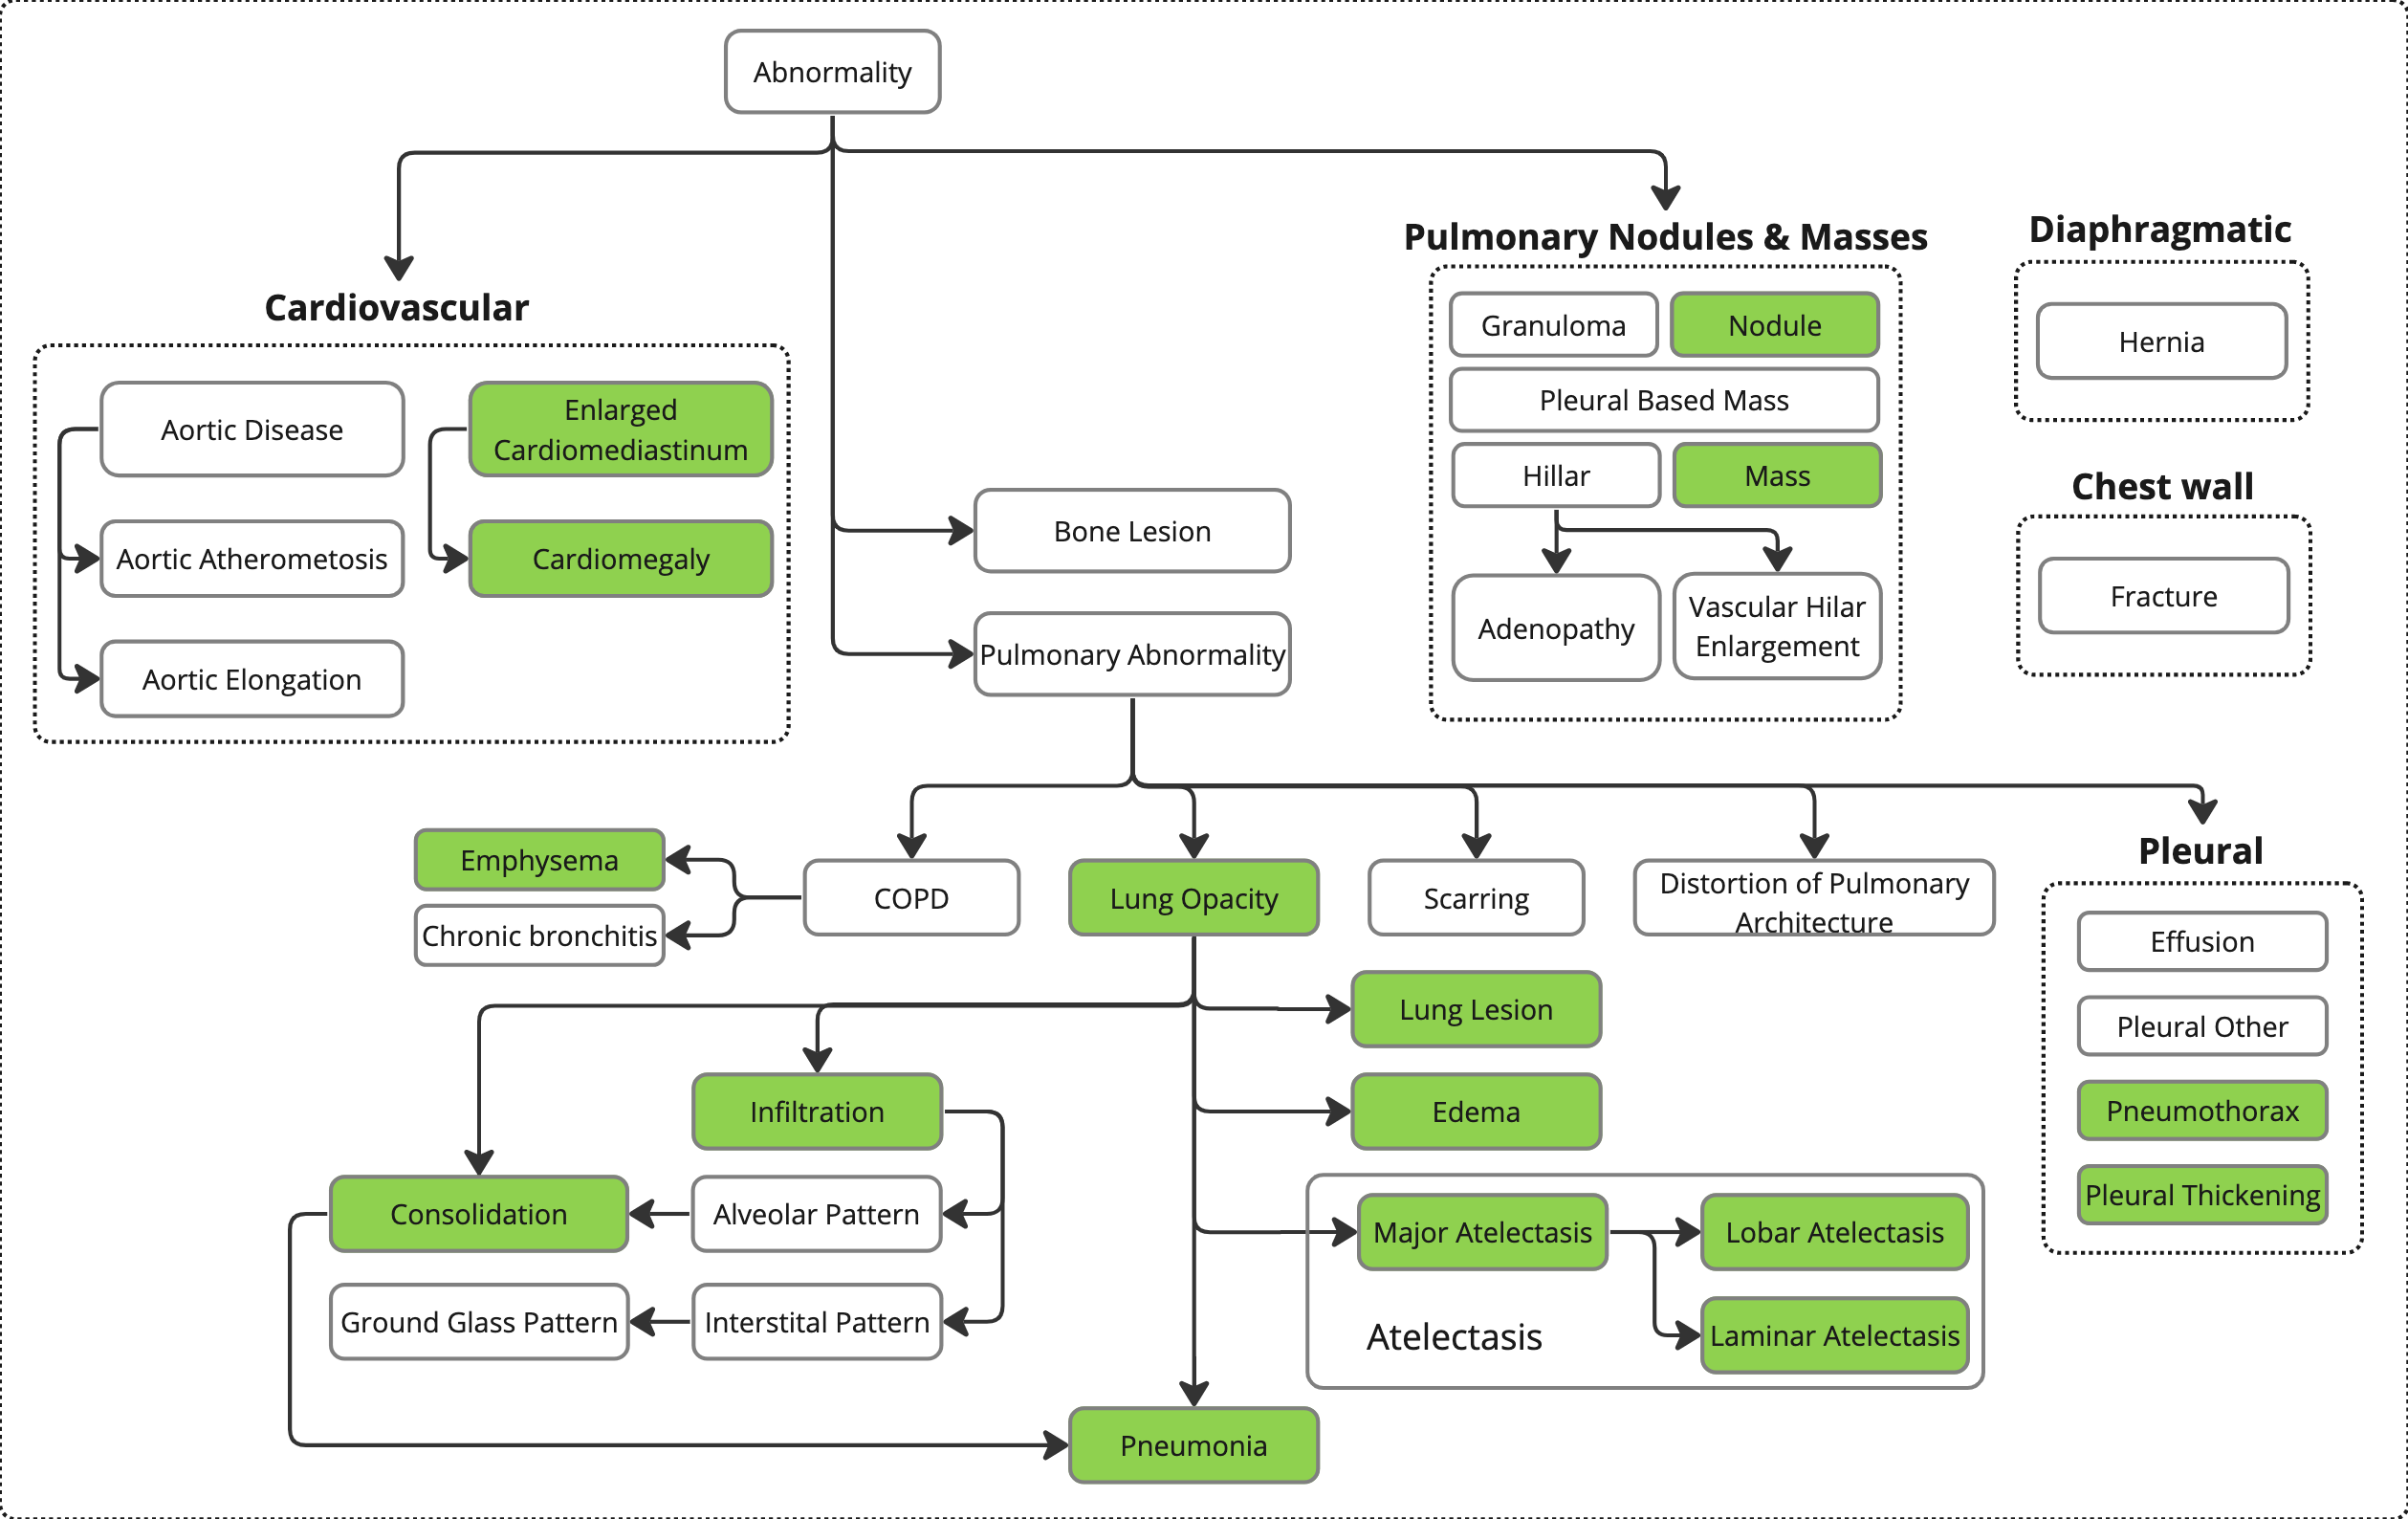
\includegraphics[width=\textwidth]{\figurepath{taxonomy_structure/taxonomy_structure}}
    \caption[Taxonomy Structure of Lung Pathologies in Chest Radiographs]{Taxonomy structure of lung pathologies in chest radiographs.}%
    \label{fig:taxonomy.fig.1.taxonomy_structure}
\end{figure}

\subsection{Datasets}
The prevalence of different pathology labels across three distinct medical imaging datasets: CheXpert~\cite{irvin_CheXpert_2019}, PADCHEST~\cite{bustos_Padchest_2020}, and NIH~\cite{wang_ChestXRay8_2017} are examined. Table~\ref{tab:taxonomy.table.1.datasets.pathologies} provides an overview of each pathology label's prevalence across these datasets. To utilize the TorchXRayVision software~\cite{cohen_TorchXRayVision_2022}, the same 18 pathologies as their work, were chosen for model fine-tuning. For the purpose of assessing the proposed methodologies, particular emphasis is placed on pathologies that are recurrent across different datasets (appear in at least two of the three datasets) and are included in our formulated taxonomy. Furthermore, the cross-dataset presence of these pathologies enhances the generalizability of our study, as the developed models are validated on multiple independent datasets. These pathologies, highlighted in \colorbox{mygreen}{green} in the table, comprise \textbf{Atelectasis}, \textbf{Consolidation}, \textbf{Infiltration}, \textbf{Edema}, \textbf{Pneumonia}, \textbf{Cardiomegaly}, \textbf{Lung Lesion}, \textbf{Lung Opacity}, and \textbf{Enlarged Cardiomediastinum}. The pathologies that are not highlighted, i.e., those occurring in just one or none of the datasets or not included in our taxonomy, were not included in the final evaluation of this study. Their exclusion is mainly due to the lack of sufficient data for a robust comparison or their non-alignment with the taxonomy structure studied.

\begin{table}[htbp]
\centering
\caption[Representation of Pathologies Across Datasets]{Representation of pathologies across datasets}%
\label{tab:taxonomy.table.1.datasets.pathologies}
\resizebox{\textwidth}{!}{\begin{tabular}{lcccrlccc}
\cellcolor[HTML]{79A8A4}{\color[HTML]{FFFFFF} \textbf{Pathologies}} & \cellcolor[HTML]{79A8A4}{\color[HTML]{FFFFFF} \textbf{NIH}} & \cellcolor[HTML]{79A8A4}{\color[HTML]{FFFFFF} \textbf{PADCHEST}} & \cellcolor[HTML]{79A8A4}{\color[HTML]{FFFFFF} \textbf{CheX}} & \textbf{} & \cellcolor[HTML]{79A8A4}{\color[HTML]{FFFFFF} \textbf{Pathologies}} & \cellcolor[HTML]{79A8A4}{\color[HTML]{FFFFFF} \textbf{NIH}} & \cellcolor[HTML]{79A8A4}{\color[HTML]{FFFFFF} \textbf{PADCHEST}} & \cellcolor[HTML]{79A8A4}{\color[HTML]{FFFFFF} \textbf{CheX}} \\
{Air Trapping} &  & X &  &  & {Hemidiaphragm Elevation} &  & X &  \\
{Aortic   Atheromatosis} &  & X &  &  & \textbf{Hernia} & X & X &  \\
{Aortic Elongation} &  & X &  &  & {Hilar Enlargement} &  & X &  \\
{Aortic   Enlargement} &  &  &  &  & {ILD} &  &  &  \\
\cellcolor[HTML]{E9ECE6}\textbf{Atelectasis} & \cellcolor[HTML]{E9ECE6}X & \cellcolor[HTML]{E9ECE6}X & \cellcolor[HTML]{E9ECE6}X &  & \cellcolor[HTML]{E9ECE6}\textbf{Infiltration} & \cellcolor[HTML]{E9ECE6}X & \cellcolor[HTML]{E9ECE6}X & \cellcolor[HTML]{E9ECE6} \\
{Bronchiectasis} &  & X &  &  & \cellcolor[HTML]{E9ECE6}\textbf{Lung Lesion} & \cellcolor[HTML]{E9ECE6} & \cellcolor[HTML]{E9ECE6} & \cellcolor[HTML]{E9ECE6}X \\
{Calcification} &  &  &  &  & \cellcolor[HTML]{E9ECE6}\textbf{Lung Opacity} & \cellcolor[HTML]{E9ECE6} & \cellcolor[HTML]{E9ECE6} & \cellcolor[HTML]{E9ECE6}X \\
{Calcified   Granuloma} &  &  &  &  & \textbf{Mass} & X & X & \\
\cellcolor[HTML]{E9ECE6}\textbf{Cardiomegaly} & \cellcolor[HTML]{E9ECE6}X & \cellcolor[HTML]{E9ECE6}X & \cellcolor[HTML]{E9ECE6}X &  & {Nodule/Mass} &  &  &  \\
\cellcolor[HTML]{E9ECE6}\textbf{Consolidation} & \cellcolor[HTML]{E9ECE6} & \cellcolor[HTML]{E9ECE6}X & \cellcolor[HTML]{E9ECE6}X &  & \textbf{Nodule} & X & X & \\
{Costophrenic   Angle Blunting} &  & X &  & \multicolumn{1}{l}{} & \textbf{Pleural Other} &  &  & X \\
\cellcolor[HTML]{E9ECE6}\textbf{Edema} & \cellcolor[HTML]{E9ECE6}X & \cellcolor[HTML]{E9ECE6}X & \cellcolor[HTML]{E9ECE6}X &  & \textbf{Pleural Thickening} & X & X &  \\
\textbf{Effusion} & X & X & X &  & \cellcolor[HTML]{E9ECE6}\textbf{Pneumonia} & \cellcolor[HTML]{E9ECE6}X & \cellcolor[HTML]{E9ECE6}X & \cellcolor[HTML]{E9ECE6}X \\
\textbf{Emphysema} & X & X &  &  & \textbf{Pneumothorax} & X & X & X \\
\cellcolor[HTML]{E9ECE6}\textbf{Enlarged   Cardiomediastinum} & \cellcolor[HTML]{E9ECE6} & \cellcolor[HTML]{E9ECE6} & \cellcolor[HTML]{E9ECE6}X & \multicolumn{1}{l}{} & {Pulmonary Fibrosis} &  &  &  \\
\textbf{Fibrosis} & X & X &  &  & {Scoliosis} &  & X &  \\
{Flattened   Diaphragm} &  & X &  &  & {Tuberculosis} &  & X &  \\
{Fracture} &  & X & X &  & {Tube} &  & X &  \\
{Granuloma} &  & X &  &  &  & \multicolumn{1}{l}{} & \multicolumn{1}{l}{} & \multicolumn{1}{l}{}
\end{tabular}}
\end{table}

The distribution of samples per pathology in each dataset is presented in Table~\ref{tab:taxonomy.table.2.datasets.ninstances}. Before applying the proposed technique, a series of preprocessing steps are performed on the ground truth label set. In the context of medical images containing multiple classes, it is a prevailing practice for the individual responsible for labeling to solely annotate the pathologies that are pertinent to their specific study requirements. Occasionally, there are situations wherein certain instances of data are classified as having specific child pathologies, but not their corresponding parent pathologies. In order to address the absence of labels for certain parent classes, which is crucial for the efficacy of the proposed techniques, we have modified the label value to signify the presence of classes with at least one child class as \textcolor{blue}{TRUE}, indicating the existence of the class in that particular instance. A preprocessing step is applied to classes that do not have corresponding labels in the original ground truth label set. In the context of this study, the Lung Opacity and Enlarged Cardiomediastinum classes are absent from the original ground truth label sets of the NIH and PADCHEST datasets (Table~\ref{tab:taxonomy.table.1.datasets.pathologies}). By revising the ground truth label set, we have identified several instances where the presence of the respective parent class can be inferred based on the presence of their respective child classes as shown in Table~\ref{tab:taxonomy.table.2.datasets.ninstances} (cells highlighted in green).
%
\begin{table}[H]
\centering
\caption[Sample Distribution Per Pathology in Evaluated Datasets (CheX, NIH, and PC)]{Sample distribution per pathology in evaluated datasets (CheX, NIH, and PC)}%
\label{tab:taxonomy.table.2.datasets.ninstances}
\begin{tabular}{lcccccc}
\rowcolor[HTML]{79A8A4}
\multicolumn{1}{c}{\cellcolor[HTML]{79A8A4}{\color[HTML]{FFFFFF} }} & \multicolumn{2}{c}{\cellcolor[HTML]{79A8A4}{\color[HTML]{FFFFFF} \textbf{CheXpert}}} & \multicolumn{2}{c}{\cellcolor[HTML]{79A8A4}{\color[HTML]{FFFFFF} \textbf{NIH}}} & \multicolumn{2}{c}{\cellcolor[HTML]{79A8A4}{\color[HTML]{FFFFFF} \textbf{PADCHEST}}} \\
\rowcolor[HTML]{79A8A4}
\multicolumn{1}{c}{\multirow{-2}{*}{\cellcolor[HTML]{79A8A4}{\color[HTML]{FFFFFF} \textbf{Pathologies\textbackslash{}Dataset}}}} & {\color[HTML]{FFFFFF} PA} & {\color[HTML]{FFFFFF} AP} & {\color[HTML]{FFFFFF} PA} & {\color[HTML]{FFFFFF} AP} & {\color[HTML]{FFFFFF} PA} & {\color[HTML]{FFFFFF} AP} \\
\textbf{Atelectasis} & 2460 & 11643 & 1557 & 1016 & 2419 & 232 \\
\textbf{Consolidation} & 1125 & 4956 & 384 & 253 & 475 & 77 \\
\textbf{Infiltration} & 0 & 0 & 3273 & 1131 & 4309 & 587 \\
\textbf{Pneumothorax} & 1060 & 4239 & 243 & 253 & 97 & 15 \\
\textbf{Edema} & 1330 & 15117 & 39 & 237 & 108 & 130 \\
\textbf{Emphysema} & 0 & 0 & 264 & 193 & 546 & 30 \\
\textbf{Fibrosis} & 0 & 0 & 556 & 61 & 341 & 8 \\
\textbf{Effusion} & 5206 & 19349 & 1269 & 654 & 1625 & 311 \\
\textbf{Pneumonia} & 992 & 2064 & 175 & 89 & 1910 & 211 \\
\textbf{Pleural\_Thickening} & 0 & 0 & 745 & 145 & 2075 & 34 \\
\textbf{Cardiomegaly} & 2117 & 8284 & 729 & 203 & 5387 & 261 \\
\textbf{Nodule} & 0 & 0 & 1609 & 460 & 2190 & 95 \\
\textbf{Mass} & 0 & 0 & 1213 & 493 & 506 & 17 \\
\textbf{Hernia} & 0 & 0 & 81 & 13 & 988 & 38 \\
\textbf{Lung Lesion} & 1655 & 3110 & 0 & 0 & 0 & 0 \\
\textbf{Fracture} & 1115 & 3463 & 0 & 0 & 1662 & 69 \\
\textbf{Lung Opacity} & 7006 & 28183 & \cellcolor[HTML]{E9ECE6}4917 & \cellcolor[HTML]{E9ECE6}2216 & \cellcolor[HTML]{E9ECE6}6947 & \cellcolor[HTML]{E9ECE6}861 \\
\textbf{Enlarged Cardiomediastinum} & 1100 & 4577 & \cellcolor[HTML]{E9ECE6}729 & \cellcolor[HTML]{E9ECE6}203 & \cellcolor[HTML]{E9ECE6}5387 & \cellcolor[HTML]{E9ECE6}261 \\
\rowcolor[HTML]{79A8A4}
{\color[HTML]{FFFFFF} Total} & {\color[HTML]{FFFFFF} 20543} & {\color[HTML]{FFFFFF} 53359} & {\color[HTML]{FFFFFF} 28868} & {\color[HTML]{FFFFFF} 9060} & {\color[HTML]{FFFFFF} 61692} & {\color[HTML]{FFFFFF} 2445}
\end{tabular}
\end{table}
%

\subsection{Techniques Evaluation}
The performance comparison of our proposed methods, namely ``logit'' and ``loss'', with the ``baseline'' technique is illustrated in Figure~\ref{fig:taxonomy.fig.3.roc_curve_all_datasets}. This comparative analysis centers on nine distinct medical conditions associated with pulmonary and cardiovascular diseases within three datasets. These nine pathologies encompass two parent classes (\textbf{Lung Opacity}, and \textbf{Enlarged Cardiomediastinum}) and their respective child classes, as illustrated in Figure~\ref{fig:taxonomy.fig.1.taxonomy_structure}. Each subplot exhibits the receiver operating characteristic (ROC) curves for each methodology superimposed on one another, accompanied by their respective AUC (Area Under Curve) scores annotated. AUC (Area Under the Curve) scores are computed for each pathology class across all test samples in all studies datasets. We can see a notable improvement in AUC scores for all pathologies possessing parent classes. The aforementioned findings serve as compelling evidence for the effectiveness of the proposed methodologies, as they showcase their ability to improve the accuracy of classification in scenarios involving hierarchical class structures. AUC scores for two parent classes, ``Lung Opacity'' and ``Enlarged Cardiomediastinum'', remain unchanged as expected. The techniques proposed in this study are designed to exploit the hierarchical structure of classes, and therefore only bring about improvements where a class possesses a parent class.


% \begin{table}[H]
% \centering
% \caption[Statistical Performance Comparison of ``Logit'', ``Loss'', and ``Baseline'' Techniques Across Various Pathologies]{Statistical performance comparison between the proposed techniques ``logit'' and ``loss'' and the ``baseline'' technique across various pathologies. The upper table displays the findings of the ``logit'' technique, while the lower table displays the findings of the ``loss'' technique. The reported metrics for each pathology are the Kappa statistic, p-value, t-statistic, statistical power, Cohen's d, and Bayes Factor (BF10). A kappa value of 1 indicates perfect agreement between techniques, whereas a larger Bayes factor indicates greater support for the ``logit'' or ``loss'' technique over the baseline.}%
% \label{tab:taxonomy.table.3.metrics}
% \resizebox{\textwidth}{!}{%
% %! suppress = EscapeAmpersand
% \begin{tabular}{clrrrrrr}
%  & \cellcolor[HTML]{79A8A4}{\color[HTML]{FFFFFF} } & \cellcolor[HTML]{79A8A4}{\color[HTML]{FFFFFF} kappa} & \cellcolor[HTML]{79A8A4}{\color[HTML]{FFFFFF} p\_value} & \cellcolor[HTML]{79A8A4}{\color[HTML]{FFFFFF} t\_stat} & \cellcolor[HTML]{79A8A4}{\color[HTML]{FFFFFF} power} & \cellcolor[HTML]{79A8A4}{\color[HTML]{FFFFFF} cohen-d} & \cellcolor[HTML]{79A8A4}{\color[HTML]{FFFFFF} BF10} \\
%  & Atelectasis & 0.495 & 2.1E-89 & 20.2 & 1 & 0.346 & 3.0E+85 \\
%  & Consolidation & 0.508 & 2.0E-18 & 8.8 & 1 & 0.150 & 8.3E+14 \\
%  & Infiltration & 0.620 & 2.7E-28 & 11.1 & 1 & 0.190 & 4.9E+24 \\
%  & Edema & 0.614 & 1.2E-52 & 15.3 & 1 & 0.263 & 7.2E+48 \\
%  & Pneumonia & 0.573 & 2.9E-16 & 8.2 & 1 & 0.140 & 6.3E+12 \\
%  & Cardiomegaly & 0.615 & 1.9E-72 & 18.1 & 1 & 0.310 & 3.9E+68 \\
%  & Lung Lesion & 0.580 & 7.0E-23 & 9.9 & 1 & 0.169 & 2.1E+19 \\
%  & Lung Opacity & 1 & 1 & 0 & 0.05 & 0 & 0.019 \\
% \multirow{-10}{*}{\begin{tabular}[c]{@{}c@{}}\\ L\\  \\ O\\ \\ G\\ \\ I\\ \\ T\end{tabular}} & Enlarged Cardiomediastinum & 1 & 1 & 0 & 0.05 & 0 & 0.019 \\
% \multicolumn{8}{l}{{\color[HTML]{FFFFFF} }} \\
%  & \cellcolor[HTML]{79A8A4}{\color[HTML]{FFFFFF} } & \cellcolor[HTML]{79A8A4}{\color[HTML]{FFFFFF} kappa} & \cellcolor[HTML]{79A8A4}{\color[HTML]{FFFFFF} p\_value} & \cellcolor[HTML]{79A8A4}{\color[HTML]{FFFFFF} t\_stat} & \cellcolor[HTML]{79A8A4}{\color[HTML]{FFFFFF} power} & \cellcolor[HTML]{79A8A4}{\color[HTML]{FFFFFF} cohen-d} & \cellcolor[HTML]{79A8A4}{\color[HTML]{FFFFFF} BF10} \\
%  & Atelectasis & 0.222 & 4.9E-183 & 29.3 & 1 & 0.502 & 7.7E+178 \\
%  & Consolidation & 0.310 & 4.3E-116 & 23.1 & 1 & 0.396 & 1.2E+112 \\
%  & Infiltration & 0.836 & \multicolumn{1}{l}{0.053} & 1.9 & 0.49 & 0.033 & 0.125 \\
%  & Edema & 0.343 & 4.4E-190 & 29.9 & 1 & 0.512 & 8.2E+185 \\
%  & Pneumonia & 0.394 & \multicolumn{1}{l}{0.207} & 1.3 & 0.24 & 0.022 & 0.043 \\
%  & Cardiomegaly & 0.501 & 1.2E-101 & 21.6 & 1 & 0.370 & 4.7E+97 \\
%  & Lung Lesion & 0.059 & 1.2E-207 & 31.3 & 1 & 0.537 & 2.9E+203 \\
%  & Lung Opacity & 1 & 1 & 0 & 0.05 & 0 & 0.019 \\
% \multirow{-10}{*}{\begin{tabular}[c]{@{}c@{}}\\ L\\ \\ O\\ \\ S\\ \\ S\end{tabular}} & Enlarged Cardiomediastinum & 1 & 1 & 0 & 0.05 & 0 & 0.019
% \end{tabular}%
% }
% \end{table}
\begin{table}[H]
\centering
\caption[Statistical Performance Comparison of ``Logit'', ``Loss'', and ``Baseline'' Techniques Across Various Pathologies]{Statistical performance comparison between the proposed techniques ``logit'' and ``loss'' and the ``baseline'' technique across various pathologies. The upper table displays the findings of the ``logit'' technique, while the lower table displays the findings of the ``loss'' technique. The reported metrics for each pathology are the Kappa statistic, p-value, t-statistic, statistical power, Cohen's d, and Bayes Factor (BF10). A kappa value of 1 indicates perfect agreement between techniques, whereas a larger Bayes factor indicates greater support for the ``logit'' or ``loss'' technique over the baseline.}%
\label{tab:taxonomy.table.3.metrics}
\resizebox{\textwidth}{!}{%
%! suppress = EscapeAmpersand
\begin{tabular}{clrrrrrr}
    & \cellcolor[HTML]{79A8A4}{\color[HTML]{FFFFFF} } & \cellcolor[HTML]{79A8A4}{\color[HTML]{FFFFFF} kappa} & \cellcolor[HTML]{79A8A4}{\color[HTML]{FFFFFF} p\_value} & \cellcolor[HTML]{79A8A4}{\color[HTML]{FFFFFF} t\_stat} & \cellcolor[HTML]{79A8A4}{\color[HTML]{FFFFFF} power} & \cellcolor[HTML]{79A8A4}{\color[HTML]{FFFFFF} cohen-d} & \cellcolor[HTML]{79A8A4}{\color[HTML]{FFFFFF} BF10} \\
    & Atelectasis & 0.495 & 0 & 20.2 & 1 & 0.346 & 10+ \\
    & Consolidation & 0.508 & 0 & 8.8 & 1 & 0.150 & 10+ \\
    & Infiltration & 0.620 & 0 & 11.1 & 1 & 0.190 & 10+ \\
    & Edema & 0.614 & 0 & 15.3 & 1 & 0.263 & 10+ \\
    & Pneumonia & 0.573 & 0 & 8.2 & 1 & 0.140 & 10+ \\
    & Cardiomegaly & 0.615 & 0 & 18.1 & 1 & 0.310 & 10+ \\
    & Lung Lesion & 0.580 & 0 & 9.9 & 1 & 0.169 & 10+ \\
    & Lung Opacity & 1 & 1 & 0 & 0.05 & 0 & 0.019 \\
\multirow{-10}{*}{\begin{tabular}[c]{@{}c@{}}\\ L\\  \\ O\\ \\ G\\ \\ I\\ \\ T\end{tabular}} & Enlarged Cardiomediastinum & 1 & 1 & 0 & 0.05 & 0 & 0.019 \\
\multicolumn{8}{l}{{\color[HTML]{FFFFFF} }} \\
    & \cellcolor[HTML]{79A8A4}{\color[HTML]{FFFFFF} } & \cellcolor[HTML]{79A8A4}{\color[HTML]{FFFFFF} kappa} & \cellcolor[HTML]{79A8A4}{\color[HTML]{FFFFFF} p\_value} & \cellcolor[HTML]{79A8A4}{\color[HTML]{FFFFFF} t\_stat} & \cellcolor[HTML]{79A8A4}{\color[HTML]{FFFFFF} power} & \cellcolor[HTML]{79A8A4}{\color[HTML]{FFFFFF} cohen-d} & \cellcolor[HTML]{79A8A4}{\color[HTML]{FFFFFF} BF10} \\
    & Atelectasis & 0.222 & 0 & 29.3 & 1 & 0.502 & 10+ \\
    & Consolidation & 0.310 & 0 & 23.1 & 1 & 0.396 & 10+ \\
    & Infiltration & 0.836 & 0.053 & 1.9 & 0.49 & 0.033 & 0.125 \\
    & Edema & 0.343 & 0 & 29.9 & 1 & 0.512 & 10+ \\
    & Pneumonia & 0.394 & 0.207 & 1.3 & 0.24 & 0.022 & 0.043 \\
    & Cardiomegaly & 0.501 & 0 & 21.6 & 1 & 0.370 & 10+ \\
    & Lung Lesion & 0.059 & 0 & 31.3 & 1 & 0.537 & 10+ \\
    & Lung Opacity & 1 & 1 & 0 & 0.05 & 0 & 0.019 \\
\multirow{-10}{*}{\begin{tabular}[c]{@{}c@{}}\\ L\\ \\ O\\ \\ S\\ \\ S\end{tabular}} & Enlarged Cardiomediastinum & 1 & 1 & 0 & 0.05 & 0 & 0.019
\end{tabular}%
}
\end{table}
The comparative analysis presented in Figure~\ref{fig:taxonomy.fig.2.metrics} examines the performance of the proposed ``loss'' and ``logit'' methods in comparison to the ``baseline'' method across three important metrics: Accuracy (ACC), Area Under the Receiver Operating Characteristic Curve (AUC), and F1 score for different pathologies.

The ``loss'' and ``logit'' methods exhibit a distinct advantage over the ``baseline'' method in terms of accuracy. In the case of Atelectasis, the ``loss'' method demonstrates a notably higher accuracy of 0.922 compared to the ``baseline'' method's accuracy of 0.686. Additionally, the ``logit'' method achieves an accuracy of 0.874. As predicted, there is no noticeable disparity in accuracy between the methods for the parent classes, Lung Opacity and Enlarged Cardiomediastinum, as indicated by scores of 0.663 and 0.696, respectively.

The AUC, a performance measure that takes into account both sensitivity and specificity, provides further evidence of the superior performance of the ``loss'' and ``logit'' techniques. In the case of Cardiomegaly, the area under the curve (AUC) demonstrates improvements of 21\% and 11\% when employing the loss and logit techniques, respectively. The AUC values for the parent classes, Lung Opacity and Enlarged Cardiomediastinum, are consistent across all three methods.

The F1 score, which is calculated as the harmonic means of precision and recall, serves to emphasize the improved performance of our proposed methods. Significantly, in the case of Lung Lesion, the F1 score exhibits a notable increase from 0.094 in the ``baseline'' approach to 0.982 in the ``loss'' approach, and 0.263 in the ``logit'' approach.

The obtained results provides further support for our previous findings, which indicate that the utilization of the ``logit'' and ``loss'' methods leads to substantial improvements in performance compared to the ``baseline'' method across most child classes. In all measured aspects and scenarios, the ``loss'' method exhibits slightly superior performance compared to the ``logit'' method.

\begin{figure}[t]
\centering
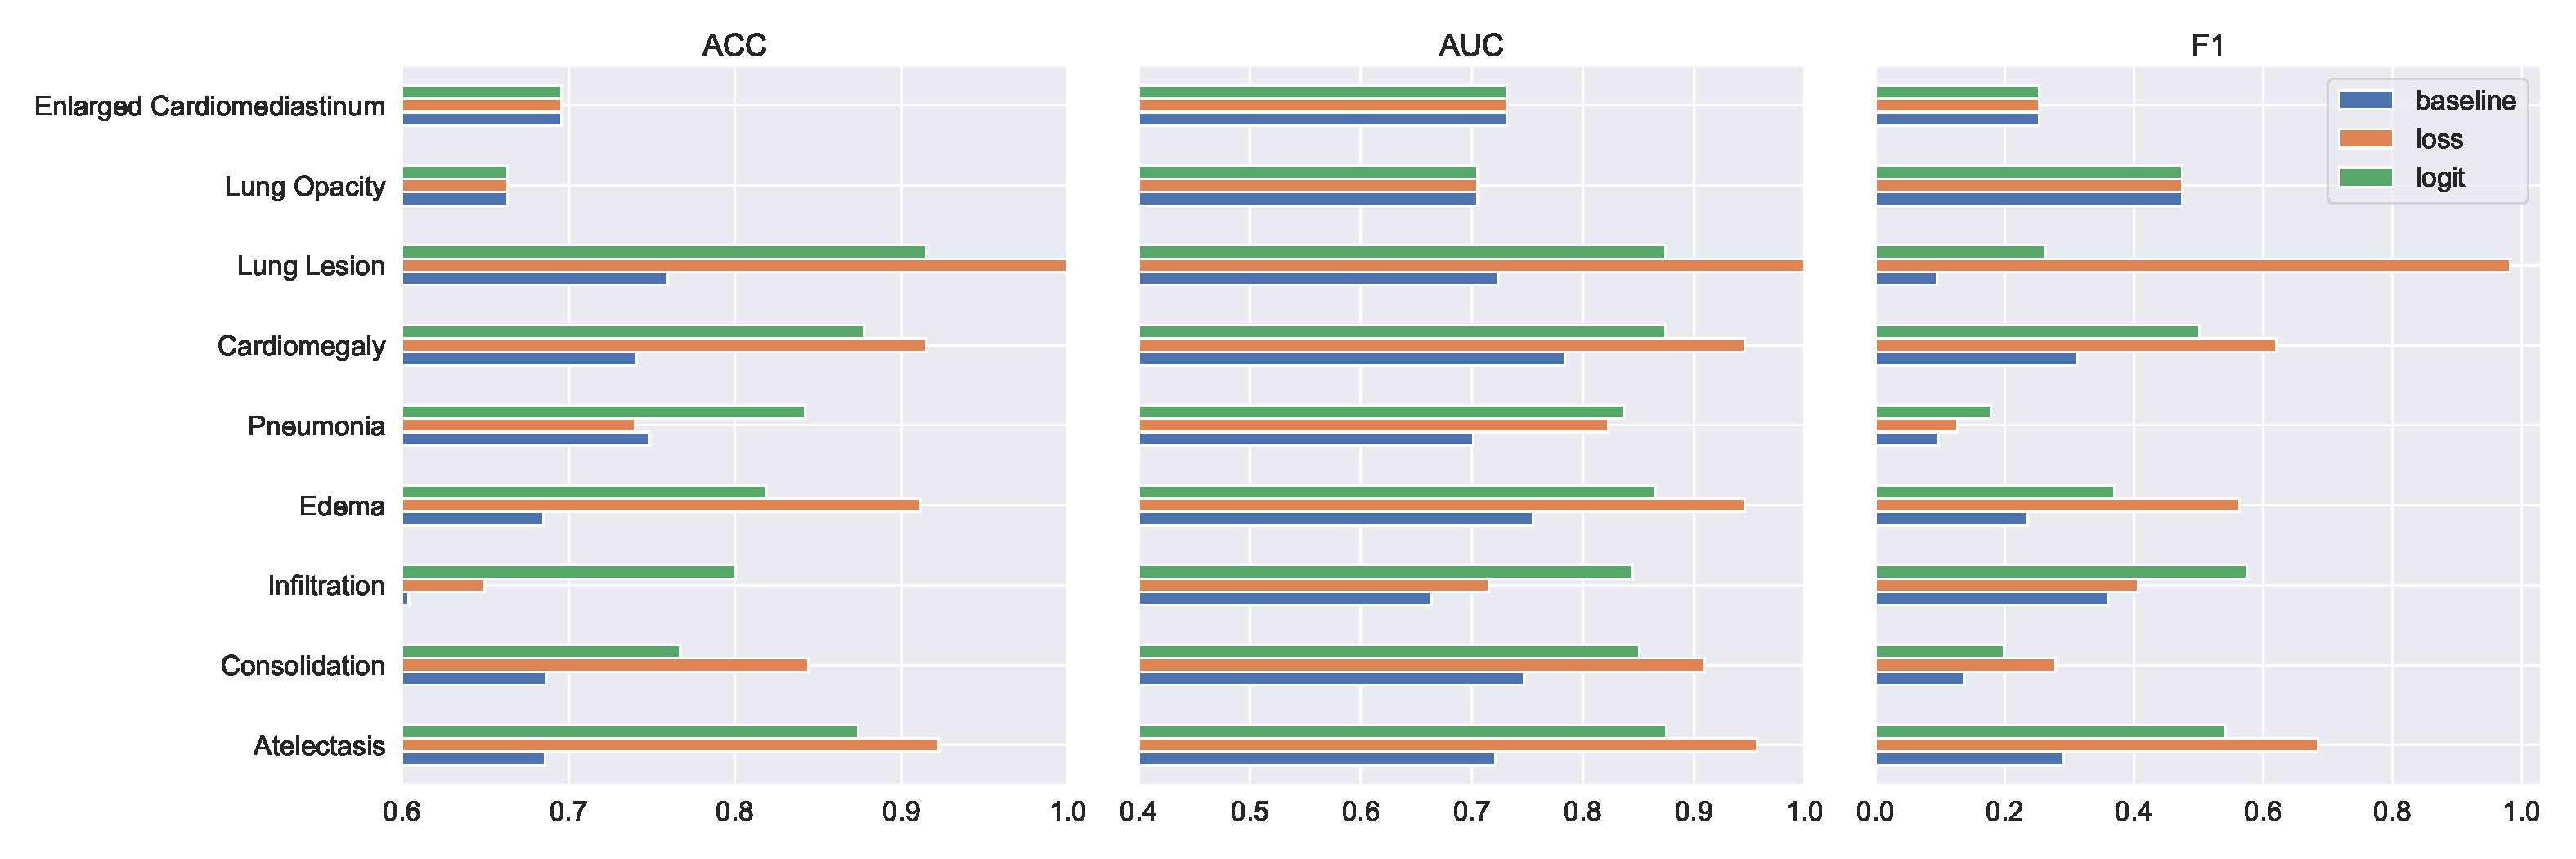
\includegraphics[width=\textwidth]{\figurepath{auc_acc_f1_all_datasets/ROC/metrics_AUC_ACC_F1}}
\caption[Heatmap Visualization of Model Performance Metrics (ACC, AUC, F1) for Different Techniques across Pathologies]{Heatmap visualization of model performance metrics across all three datasets. The subplots from left to right correspond to the Accuracy (ACC), Area Under the ROC Curve (AUC), and F1 Score for the baseline, ``loss'', and ``logit'' techniques respectively. The pathologies are shared on the y-axis. Darker colors signify higher values, indicating better model performance. Each cell represents the value of the corresponding metric for the given technique on a specific pathology}\label{fig:taxonomy.fig.2.metrics}
\end{figure}

\begin{figure}[t]
\centering
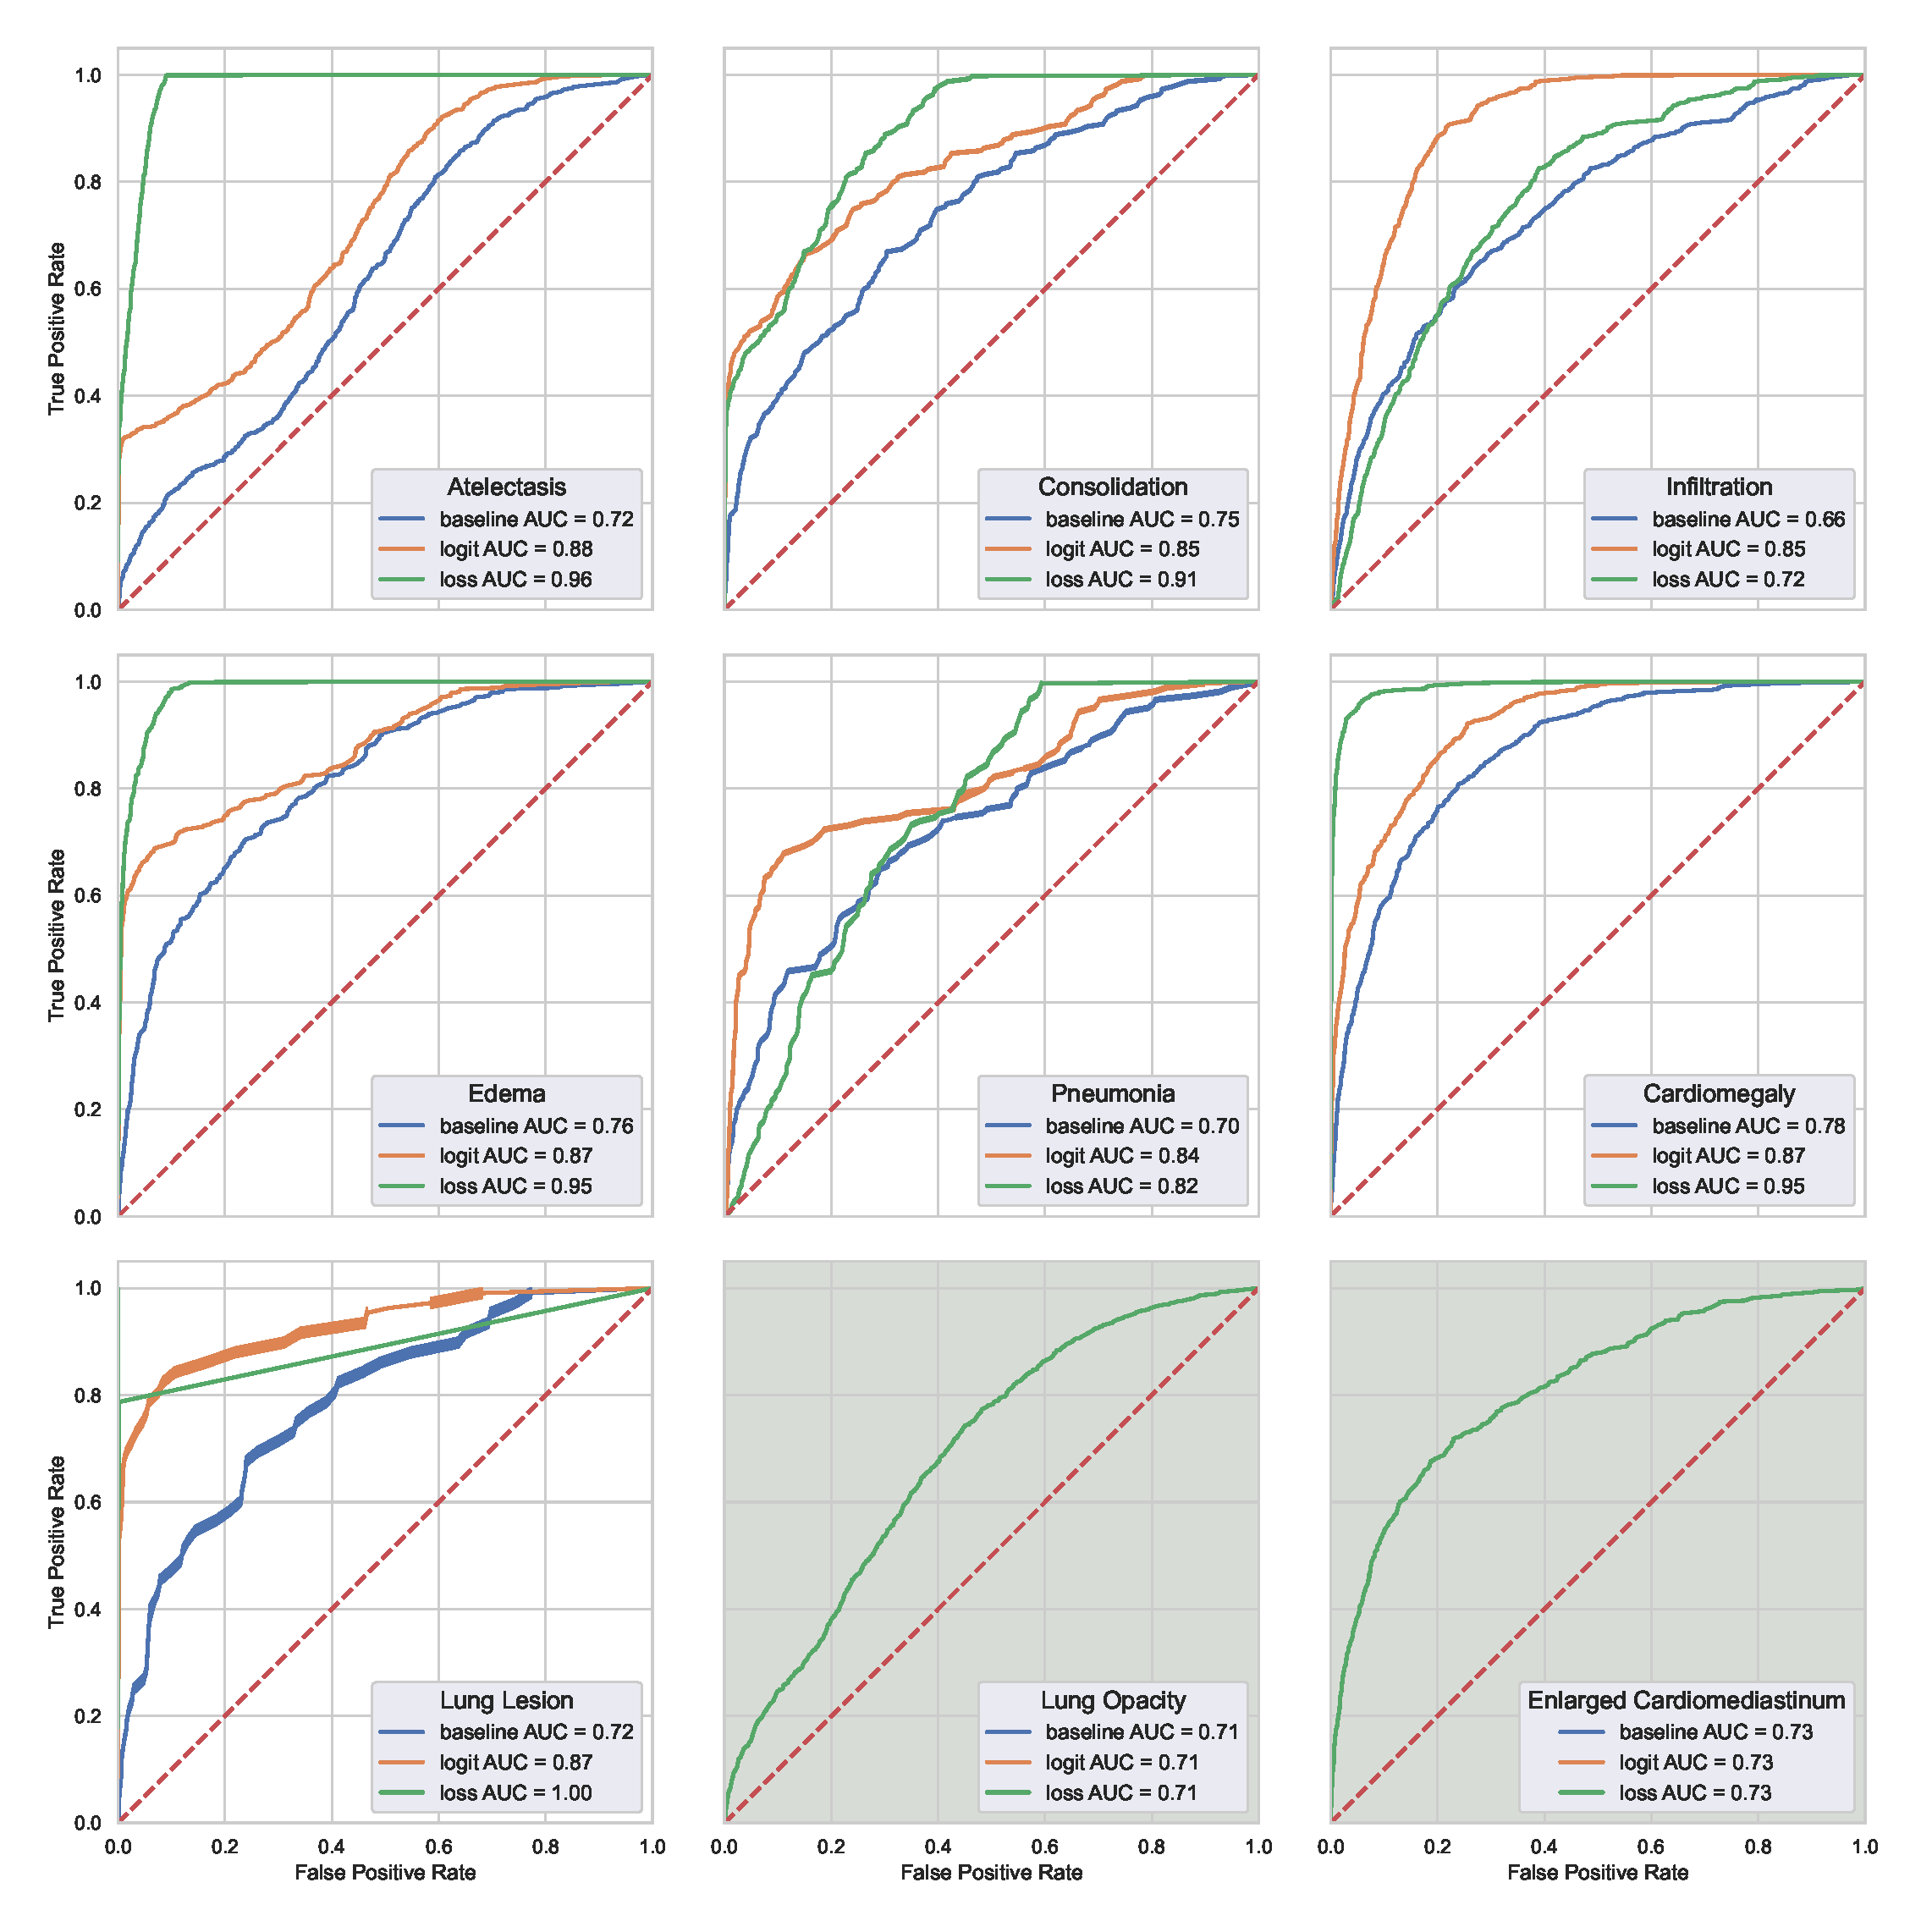
\includegraphics[width=\textwidth]{\figurepath{roc_curve_all_datasets/ROC/roc_curve_all_datasets}}
\caption[Comparative Analysis of ROC Curves for Nine Thoracic Pathologies: ``logit'', ``loss'', and ``baseline'' Techniques]{Comparative analysis of the ROC curves for nine thoracic pathologies using the ``logit'' and ``loss'' techniques as well as the baseline. The subplots highlighted with a darker background, represent parent class diseases.}\label{fig:taxonomy.fig.3.roc_curve_all_datasets}
\end{figure}

Table~\ref{tab:taxonomy.table.3.metrics} provides a comparative analysis of the performance of our proposed ``logit'' and ``loss'' techniques with the ``baseline'' method, using various statistical metrics. The ``logit'' technique, as indicated in the upper table, suggest a significant performance enhancement compared to the ``baseline'' across all evaluation tests, with kappa values ranging between 0.495 and 1. The kappa statistic is used to measure the level of agreement between two techniques, where a value of 1 signifies perfect alignment. The p-value for all child classes is below 0.05, ranging from 2.1E-89 to 2.9E-16, thereby implying a statistically significant improvement of the ``logit'' method over the ``baseline''. High t-statistics and power values of 1 further underscore the robustness of our technique. The Bayes factor results for the ``logit'' technique are exceptionally strong across all classes, suggesting substantial evidence favoring the ``logit'' method for these scenarios.

The proposed ``loss'' technique demonstrates encouraging results when benchmarked against the ``baseline'', albeit with more variability. Kappa values spanned from a minimum of 0.059 for Lung Lesion to a maximum of 0.836 for Infiltration. While the p-values indicate statistically significant improvement for most conditions, Infiltration and Pneumonia had p-values exceeding 0.05 (0.053 and 0.207, respectively), hinting that the performance improvement over the ``baseline'' for these conditions may not be statistically significant. High t-statistics and power values of 1 were observed for all conditions except Infiltration and Pneumonia. The cohen-d values for the ``loss'' technique were generally larger than those for the ``logit'' technique, signifying a larger effect size. The Bayes factor results for the ``loss'' technique were exceedingly strong for conditions such as Atelectasis and Edema, but considerably lower for conditions like Infiltration and Pneumonia, indicating less evidence supporting the ``loss'' technique for these conditions.

Both the ``logit'' and ``loss'' techniques shows considerable improvements over the ``baseline'' technique, though the degree of improvement varied. The ``logit'' technique exhibited a more consistent level of improvement across all conditions, whereas the ``loss'' technique showed potential for even larger improvements in certain conditions, albeit with less consistency across the conditions studied.

\section{Discussion and Conclusion}\label{sec:taxonomy.discussion}
%
In this research, we introduce two innovative hierarchical multi-label classification techniques designed to increase both the accuracy and understandability of results in applications where a hierarchical structure exists among classes. The techniques are intended to improve classification accuracy, resistance to labeling inaccuracies and enhance alignment with hierarchical class structures. The proposed ``loss'' technique is devised to be integrated into any loss function (e.g., binary cross entropy loss) that is used for optimizing the model parameters, enabling a more refined adjustment of the hierarchical influence through introducing a regularization term in the loss function of the model. The proposed ``logit'' technique offers a straightforward yet potent method to integrate label hierarchy into a model without necessitating considerable changes to the existing structure.
%
Our results affirm the effectiveness of the introduced hierarchical multi-label classification techniques in increasing the classification accuracy of thoracic diseases. Several performance indicators, including accuracy, AUC, and F1 scores, along with Cohen's d, Cohen's kappa, t-statistics, p-value, and Bayes factor, attest to the substantial performance improvements of these methods over the baseline across three major public datasets (CheXpert, PADCHEST, and NIH). These findings suggest that the proposed techniques can be more reliable tools for improving classification accuracy as well as a higher level of interpretability in the findings.
%
The ``loss'' and ``logit'' techniques harness the disease taxonomy to enhance classification performance, underscoring the value of using label relationships in classification tasks. These hierarchical techniques could potentially aid healthcare professionals by enhancing the comprehensibility of the model's predictions. Providing predictions with varying detail levels based on taxonomy could enable personalized diagnoses that better meet individual clinical needs. Moreover, the techniques could be integrated into computer-aided diagnosis systems to deliver more precise and efficient diagnoses, possibly reducing clinicians' workload and improving patient outcomes.
%
However, further research is needed to explore their potential benefits in a clinical setting. There are also some limitations to these methods. For example, applying these techniques to other applications would necessitate the creation of a taxonomical structure for the dataset labels, which could be challenging for complex applications and usually requires consensus among several domain experts. Also, the effectiveness of the introduced techniques could be influenced by the quality and consistency of dataset labeling, which may vary across different sources. Future research should aim to evaluate these techniques across a broader array of datasets and investigate the impact of labeling quality on performance.
%

\section*{Appendices}

\section*{Acknowledgements}



\section{Introduction}\label{sec:crowd.Introduction}
Supervised learning techniques require a large amount of labeled data to train models to classify new data~\cite{jiang_Wrapper_2019,jiang_Class_2019}. Traditionally, data labeling has been assigned to experts in the domain or well-trained workers~\cite{tian_MaxMargin_2019}. Although this method produces high-quality labels, it is inefficient and costly~\cite{li_Noise_2016,li_Noise_2019}.  Social networking provides an innovative solution to the labeling problem by allowing data to be labeled by online crowd workers (annotators). This has become feasible, as crowdsourcing services such as Amazon Mechanical Turk (formerly CrowdFlower) have grown in popularity. Crowdsourcing systems have been used to accumulate large amounts of labeled data for applications such as computer vision~\cite{deng_ImageNet_2009,liu_Variational_2012} and natural language processing~\cite{karger_Budget_2014}. However, because of individual differences in preferences and cognitive abilities, the quality of labels acquired by a single crowd worker is typically low, thus jeopardizing applications that rely on these data. This is because crowd workers are not necessarily domain experts and may lack the necessary training or expertise to produce high-quality labels.

Aggregation after repeated labeling is one method for handling workers with various abilities. Label aggregation is a process used to infer an aggregated label for a data instance from a multi-label set~\cite{sheshadri_SQUARE_2013}. Several studies have demonstrated the efficacy of repeated labeling~\cite{tu_MultiLabel_2018,zhang_multilabelinferencecrowdsourcing_2018}. Repeat labeling is a technique in which the same data are labeled by multiple workers, and the results are combined to estimate an aggregated label using majority voting (MV) or other techniques. In the case of MV, an aggregated label is the label that receives the most votes from the workers for a given data instance. This can help reduce the impact of biases or inconsistencies made by workers. Several factors, such as problem-specific characteristics, the quality of the labels created by the workers, and the amount of data available, can influence the effectiveness of the aggregation methodologies. Consequently, it is difficult to identify a clear winner among the different techniques. For example, in binary labeling, one study~\cite{sheshadri_SQUARE_2013} discovered that Raykar's~\cite{raykar_Learning_2010} technique outperformed other aggregation techniques. However, according to another study~\cite{zheng_Truth_2017}, the traditional Dawid-Skene (DS) model~\cite{dawid_Maximum_1979} was more reliable in multi-class settings (where data instances can be labeled as belonging to multiple classes).

Furthermore, regardless of the aggregation technique used, the performance of many aggregation techniques in real-world datasets remains unsatisfactory~\cite{liu_Exploiting_2021}. This can be attributed to the complexity of these datasets, which often do not align with the assumptions and limitations of different methods. For example, real-world datasets may present issues such as labeling inaccuracies, class imbalances, or overwhelming sizes that challenge efficient processing with available resources. These factors can adversely affect the effectiveness of label aggregation techniques, potentially yielding less than optimal results for real-world datasets.
Prior information may be used to enhance the label aggregation procedure.

This can include domain knowledge, the use of quality control measures, and techniques that account for the unique characteristics of workers and data. Knowing the reliability of certain workers, it is possible to draw more accurate conclusions about labels~\cite{li_Crowdsourced_2017}. For instance, in the label aggregation process, labels produced by more reliable workers (such as domain experts) may be given greater weight. The results of the label aggregation process can also be validated using expert input~\cite{liu_Improving_2017}. During the labeling process, domain experts can provide valuable guidance and oversight to ensure that the labels produced are accurate and consistent.
The agnostic requirement for general-purpose label aggregation is that label aggregation cannot use information outside the labels themselves. This requirement is not satisfied in most label aggregation techniques~\cite{zhang_Crowdsourced_2019}. The agnostic requirement ensures that the label aggregation technique is as general as possible and applicable to a wide range of domains with minimal or no additional context.

The uncertainty of workers during labeling can provide valuable prior knowledge to determine the appropriate amount of confidence to grant each worker while still adhering to the requirement of a general-purpose label aggregation technique. We developed a method for estimating the reliability of different workers based on the worker's own consistency during labeling. We take this concept a step further by calculating a weight for each worker based not only on their reliability but also on their agreements with other workers involved. This consideration of inter-reliability ensures a more comprehensive and dynamic weighting process, adjusting to the overall performance of the entire group of workers. Thus, the generated weights become a measure of both individual and collective reliability, which significantly improves the accuracy of our labeling aggregation method.

We introduce a novel method, named Crowd-Certain, which offers a significant improvement in label aggregation for crowdsourced and ensemble learning classification tasks, yielding improved performance across various scenarios. This technique leverages the consistency of workers versus a trained classifier to ascertain their reliability, resulting in more accurate and efficient label aggregation.

Our extensive experimental evaluation, conducted across ten diverse datasets, demonstrates that Crowd-Certain outperforms established techniques (Gold Majority Vote, MV, MMSR, Wawa, Zero-Based Skill, GLAD, and Dawid Skene) in terms of aggregated label accuracy compared to ground truth labels. Importantly, Crowd-Certain generates weights that closely follow pre-set ground truth accuracy for each worker (referred to as a probability threshold in this study). Moreover, during inference time, Crowd-Certain employs predicted probabilities (obtained from a classifier trained on the worker's label set) rather than worker's labels, which facilitates the reuse of trained classifiers for future data samples, removing the need for repeating the training process when new data samples are introduced.
The remainder of this paper is organized as follows. Section~\ref{sec:crowd.relatedwork} examines related work involving label aggregation algorithms. In Section~\ref{sec:crowd.method}, we provide an in-depth explanation of Crowd-Certain. Section~\ref{sec:crowd.results} presents the experiments and findings, and Section~\ref{sec:crowd.discussion} encapsulates the results, highlighting key insights. Lastly, Section~\ref{sec:crowd.conclusion} concludes the paper and highlights the potential directions for future research.

\section{Related Work}\label{sec:crowd.relatedwork}
Numerous label aggregation algorithms have been developed to capture the complexity of crowdsourced labeling systems, including techniques based on worker reliability~\cite{bi_Learning_2014,demartini_Zencrowd_2012}, confusion matrices~\cite{raykar_Learning_2010,zhang_Spectral_2014}, intentions~\cite{bi_Learning_2014,kurve_MultiCategory_2015}, biases~\cite{zhang_Imbalanced_2013,hernandez-gonzalez_Note_2019, welinder_Multidimensional_2010}, and correlations~\cite{ma_Gradient_2020}. However, because crowdsourced labeling is inherently dynamic and uncertain, developing a technique that can work in most situations is extremely challenging. Many techniques~\cite{liu_Variational_2012,karger_Budget_2014,raykar_Learning_2010,dalvi_Aggregating_2013,ghosh_Who_2011} utilize the Dawid and Skene (DS) generative model~\cite{dawid_Maximum_1979}. Ghosh~\cite{ghosh_Who_2011} extended the DS model by using singular value decomposition (SVD) to calculate the reliability of the worker. Similarly, to Ghosh~\cite{ghosh_Who_2011}, Dalvi~\cite{dalvi_Aggregating_2013} used SVD to estimate true labels with a focus on the sparsity of the labeling matrix. In crowdsourcing, it is common for the labeling matrix to be sparse, meaning that not all workers have labeled all the data. This may be due to several factors, such as the cost of labeling all data instances or the workers' time constraints. Karger~\cite{karger_Budget_2014} described an iterative strategy for binary labeling based on a one-coin model~\cite{ghosh_Who_2011}. Karger~\cite{karger_Budget_2014} extends the one-coin model to multi-class labeling by converting the problem into $k-1 $ binary problems (solved iteratively), where $k $ is the number of classes.

The MV technique assumes that all workers are equally reliable. For segmentation, Warfield~\cite{warfield_Simultaneous_2004} proposed simultaneous truth and performance level estimation (STAPLE), a label fusion method based on expectation maximization. STAPLE ``weighs'' expert opinions during label aggregation by modeling their reliability. Since then, many variants of this technique have been proposed~\cite{winzeck_ISLES_2018,commowick_Objective_2018,asman_Robust_2011,asman_Formulating_2012, eugenioiglesias_Unified_2013, jorgecardoso_STEPS_2013,asman_NonLocal_2013,akhondi-asl_Logarithmic_2014}. The problem with these label aggregation approaches is that they require the computation of a unique set of weights for each sample, necessitating the re-evaluation of the workers' weights when a new instance is added.

Among the numerous existing label aggregation strategies, MV remains the most efficient and widely used approach~\cite{tao_Label_2020}. If we assume that all workers are equally reliable and that their errors are independent of one another, then, according to the theory of large numbers, the likelihood that the MV is accurate increases as the number of workers increases. However, the assumption that all workers are equally competent and independent may not always hold. Furthermore, MV does not provide any additional information on the degree of disagreement among the workers (As an example, consider the scenario where four of seven doctors think patient A needs immediate surgery, while all seven think patient B needs immediate surgery; MV will simply label ``yes'' in both cases).
To address this problem, additional measures such as inter-worker agreements (IAA) have been used~\cite{artstein_InterAnnotator_2017}. IAA is a measurement of the agreement among multiple workers who label the same data instance. Typically, IAA is calculated using statistical measures, such as Cohen's kappa, Fleiss's kappa, or Krippendorff's alpha~\cite{krippendorff_Content_2018}. These measures consider both the observed agreement between the workers and the expected agreement owing to random chance. IAA can also be visualized using a confusion matrix or annotation heatmap, which illustrates the distribution of labels assigned by the workers. This can help identify instances where the workers disagree or are uncertain and can guide further analysis to improve the annotation~\cite{carletta_Assessing_1996}.

Recently, Sheng~\cite{sheng_Majority_2019} proposed a technique that provided a confidence score along with an aggregated label. The main problem with this approach is that it assumes that all workers are equally capable when calculating the confidence score. Tao~\cite{tao_Label_2020} improved Sheng's approach by assigning different weights to workers for each instance. This weighting method combines the specific quality $s_\alpha^{(i,k)} $ for the worker $\alpha $ and instance $i $ and the overall quality $\tau_\alpha$ across all instances.

Inspired by Li's technique~\cite{li_Incorporating_2018}, Tao evaluates the similarity between the worker labels for each instance. To derive the specific quality $s_{\alpha}^{(i)}$, Tao counts the number of workers who assigned the same label as the worker $\alpha $ for that instance. To calculate the overall quality $\tau_\alpha $, Tao performs a 10-fold cross-validation to train each of the 10 classifiers on a different subset of data using the labels provided by the worker $\alpha $ as true labels and then assigns the average accuracy of the classifiers across all remaining instances as $\tau_\alpha $. The final weight for worker $\alpha $ and instance $i $ is then calculated using the sigmoid function $\gamma_{i,\alpha}=\tau_\alpha\left(1+{\left(s_{\alpha}^{(i)}\right)}^{2}\right) $. However, Tao's technique~\cite{tao_Label_2020} has some drawbacks. It relies on the labels of other workers to estimate $s_{\alpha}^{(i)} $. However, different workers have varying levels of competence (reliability) when labeling the data, and therefore, relying on their labels to measure $s_{\alpha}^{(i)} $ will result in propagating the errors and biases of their labels during weight estimation. Furthermore, Tao's technique~\cite{tao_Label_2020} relies on the labels provided by each worker $\alpha $ to estimate their respective $\tau_\alpha $ by assuming that the trained classifiers can learn the inherent characteristics of the datasets even in the absence of ground truth labels. While that may be true in some cases, it typically leads to suboptimal measurement and the propagation of biases and errors, from both the worker's labels and the classifier, into weight estimation.

\section{Methods}\label{sec:crowd.method}
We propose a novel method called Crowd-Certain which focuses on leveraging uncertainty measurements to improve decision-making in crowdsourcing and ensemble learning scenarios. Crowd-Certain employs a weighted soft majority voting approach, where the weights are determined based on the uncertainty associated with each worker's labels. Initially, we use uncertainty measurement techniques to calculate the degree of consistency of each worker during labeling.

Furthermore, to ensure that the proposed technique does not calculate a high weight for workers who are consistently wrong (for example, when a specific worker always mislabels a specific class, and hence demonstrates a high consistency even if they label instances incorrectly), we extend the proposed technique by penalizing the workers for instances in which they disagree with the aggregated label obtained using MV. To mitigate the reliance on training a classifier on an worker's labels, which may be inaccurate, we train an ensemble of classifiers for each worker. In addition, we report two confidence scores along with the aggregated label to provide additional context for each calculated aggregate label. We report a single weight for all instances in the dataset. As will be demonstrated in Section~\ref{sec:crowd.results}, the proposed Crowd-Certain method is not only comparable to other techniques in terms of accuracy of the aggregated labels with respect to the ground truth labels for scenarios with a large number of workers, but also provides a significant improvement in accuracy for scenarios where the number of workers may be limited. Furthermore, by assigning a single weight to each worker for all instances in the dataset, the model can assign labels to new test instances without recalculating the worker weights. This is especially advantageous in situations where workers are scarce as it enables the model to make accurate predictions with minimal dependence on worker input. This characteristic of the Crowd-Certain method can significantly reduce the time and resources required for labeling in practical applications. When deploying the model in real-world scenarios such as medical diagnosis, fraud detection, or sentiment analysis, it could be advantageous to be able to assign labels to new instances without constantly recalculating worker weights.

\subsection{Glossary of Symbols}
For convenience, the following list summarizes the major symbols used in the subsequent discussion:
\begin{itemize}{
    \setlength{\parindent}{1.5em}
    % \renewcommand{\textbullet}{}
    \item  $N$: Number of instances.
    \item  $M$: Number of workers.
    \item  $y^{(i,k)} \in \{0,1\} $: True label for the $k $-th class for instance $i $.
    \item  $z_\alpha^{(i,k)} \in \{0,1\} $: Label given by worker $\alpha $ for $k $-th class for instance $i $.
    \item  ${{\underset\alpha{\mathrm{MV}}}{\left(z_\alpha^{(i,k)}\right)}} $: Majority voting technique (the label that receives the most votes) applied to worker labels for class $k $ and instance $i $.
    \item  $\pi_\alpha^{(k)} $: Probability threshold used as a pre-set ground truth accuracy, for each worker $\alpha$ and class $k$. It is used to generate sample binary labels (fictitious ground truth label set) for worker $\alpha $ for class $k $. For example, the threshold values may be obtained from a uniform distribution in the interval $0.4 $ to $1 $, i.e., $\pi_\alpha^{(k)} \sim U(0.4,1) $.
    \item  $X^{(i)} $: Data for instance $i$.
    \item  $Y^{(i)}=\left\{y^{(i,1)},y^{(i,2)},\;\dots,y^{(i,K)}\right\} $: True label set, for instance $i $. For example, consider a dataset that is labeled for the presence of cats, dogs, and rabbits in any given instance. If a given instance $X^{(i)} $ has cats and dogs but not rabbits, then $Y^{(i)}=\{1,1,0\} $.
    \item  $Z_{\alpha}^{(i)}=\left\{z_\alpha^{(i,1)}, z_\alpha^{(i,2)}, \dots, z_\alpha^{(i,K)}\right\} $: Label set given by the worker $\alpha $ for instance $i $.
    \item $K$: number of categories (aka classes) in a multi-class multi-label problem. For example, if we have a dataset labeled for the presence of cats, dogs, and rabbits in any given instance, then $K=3$.
    \item  $\rho^{(i)}$: Randomly generated number  between 0 and 1 for instance $i $. It is obtained from a uniform distribution, i.e., $\rho^{(i)} \sim U(0,1) $ This number is used to determine, for each instance $i$, whether the true label should be assigned to each fictitious worker's label. For each class $k$, if the worker's probability threshold $\pi_\alpha^{(k)}$ is greater than $\rho^{(i)}$, the true label $y^{(i,k)}$ is assigned; otherwise, an incorrect label $1 - y^{(i,k)}$  is assigned.
    \item  $\Pi_\alpha=\left\{ \pi_\alpha^{(1)} , \pi_\alpha^{(2)}  , \dots, \pi_\alpha^{(K)} \right\} $: set of $K $ probability thresholds for worker $\alpha $.
    \item  $\mathbb{X}={\left\{X^{(i)}\right\}}_{i=1}^{N} $: Set of all instances.
    \item  $\mathbb{Y} = {\left\{Y^{(i)}\right\}}_{i=1}^{N} $: Set of all true labels.
    \item  $\mathbb{Z}_\alpha = {\left\{Z_\alpha^{(i)}\right\}}_{i=1}^{N} $: Set of all labels for the worker $\alpha $.
    \item  $\mathbb{P} = {\left\{\rho^{(i)}\right\}}_{i=1}^{N} $: Set of $N $ randomly generated numbers.
    \item  $\mathbb{D}=\left\{\mathbb{X},\mathbb{Y}\right\} $: Dataset containing all instances and all true labels.
    \item  $\mathbb{D}_\alpha=\left\{\mathbb{X},\mathbb{Z}_\alpha\right\} $: Dataset containing the labels given by the worker $\alpha $.
    \item  $f_{\alpha}^{(g)}(\cdot)$: Classifier $g $ trained on dataset $\mathbb{D}_{\alpha}^{\mathrm{train}} $ with random seed number $g $ (which is also the classifier index)
    \item  $P_{\alpha}^{(i),(g)} = {\left\{ p_{\alpha}^{(i,k),(g)} \right\}}_{k=1}^{K} $: Predicted probability set obtained in the output of the classifier $f_{\alpha}^{(g)}(\cdot) $ representing the probability that each class $k $ is present in the sample.
    \item  $\theta_{\alpha}^{(k),(g)} $: Binarization threshold. To obtain this, we can utilize any existing thresholding technique. For example, in one technique, we analyze the ROC curve and find the corresponding threshold where the difference between the true positive rate (sensitivity) and false positive rate (1-specificity) is maximum. Alternatively, we could simply use $0.5 $.
    \item  $t_\alpha^{(i,k),(g)} =
        \begin{cases}
            1 & \text{if } p_\alpha^{(i,k),(g)} > \theta_\alpha^{(k),(g)}, \\
            0 & \text{otherwise}.
        \end{cases} $: Predicted label obtained by binarizing $p_\alpha^{(i,k),(g)} $.
    \item  $\eta_{\alpha}^{(i,k)} = {{\underset g{\mathrm{MV}}}{ \left(t_\alpha^{(i,k),(g)}\right) }} $: The output of the majority vote applied to the predicted labels obtained by the $G $ classifiers.
    \item  $\Delta_{\alpha}^{(i,k)} $: Uncertainty score.
    \item  $c_\alpha^{(i,k)} $: Consistency score.
    \item  $\omega_\alpha^{(k)} $: Estimated weight for worker $\alpha $ and class $k $.
    \item  $\nu^{(i,k)} = \frac{1}{{M}}{\sum_{\alpha}{\omega_\alpha^{(k)} \; \eta_\alpha^{(i,k)}}}$: Final aggregated label for class $k $ and instance $i $.
    }
\end{itemize}
\subsection{Risk Calculation}
Label aggregation is frequently used in various machine learning tasks, such as classification and regression, when multiple workers assign labels to the same data points. The aggregation model refers to the underlying function that maps a set of multiple labels, obtained by different workers, into one aggregated label. In the context of label aggregation, this model can be a neural network, a decision tree, or any other machine learning algorithm capable of learning to aggregate labels provided by multiple workers. The objective of this study is to develop an aggregation model capable of accurately determining true labels despite potential disagreements among workers. One common method to achieve this involves minimizing the total error (or disagreement) between the workers' assigned labels and the true labels, as follows:
\begin{equation}
    E = \sum_{i=1}^N \sum_{a=1}^M \left( \sum_{k=1}^K \delta\left(y^{(i,k)}, z_\alpha^{(i,k)}\right) \right)
    \label{eq:crowd.Eq.1.risk.error}
\end{equation}
where $\delta $ is the Kronecker delta function.

Although error is a crucial aspect in determining the aggregation model's performance, it treats false positives and false negatives with equal weight. However, in many practical scenarios, it is essential to weigh false positives and false negatives differently depending on the specific context and potential consequences of each type of misclassification. The concept of risk allows us to achieve this by incorporating a loss function, which assigns different weights to different types of errors. In this way, risk serves as a weighted calculation of error, enabling us to better evaluate the performance of an aggregation model and its generalization capability.

Let us denote loss function, $\mathcal{L}(\cdot)$, as a function that quantifies the discrepancy between the predicted labels and the true labels, accounting for the varying importance of different types of errors. Risk, denoted as $R(h) $, represents the expected value of a loss function over all possible data instances.  In practice, our goal is to minimize the risk to achieve optimal performance on unseen data. However, since we only have access to a limited dataset (empirical distribution), we instead work with the empirical risk. This limitation may arise because of the need to reserve a portion of our data for testing and validation or because no dataset can fully capture all possible data instances in the real world. However, minimizing risk alone could result in overfitting, in which the aggregation model learns the noise in the training data rather than the underlying patterns, resulting in poor generalization to unseen data. To improve generalizability, it is necessary to employ regularization techniques to strike a balance between the complexity of the aggregation model and its ability to fit the training data.

Risk measurement enables us to assess the aggregation model's performance in terms of accuracy (of the aggregated labels with respect to the ground truth labels), overfitting (when risk is minimized, but the model performs poorly on unseen data), and model complexity. Assume that the aggregation model $h (\cdot) $ is a function that takes a set of $M $ label sets $Z^{(i)} $ for each instance $i $ in the training data and calculates an aggregated label set $\widehat{Y}^{(i)} $ as an estimate of the true label set $Y^{(i)} $. Our goal is to find an aggregation model $h(\cdot) $ that minimizes risk defined as follows:
\begin{equation}
    R(h) = \frac{1}{N} \sum_{i=1}^{N} \mathcal{L} \left( Y^{(i)}, h\left({\left\{Z_{\alpha}^{(i)}\right\}}_{\alpha=1}^{M}\right)\right)
    \label{eq:crowd.Eq.2.risk.emp}
\end{equation}
In this context, $\mathcal{L}(\cdot) $ represents an arbitrary loss function, which quantifies the discrepancy between predicted labels and true labels while accounting for the varying importance of different types of errors.
Our goal is to choose an aggregation model $\widehat{h} $ that minimizes the risk, following the principle of risk minimization~\cite{vapnik_Principles_1991}:
\begin{equation}
    \widehat{h} = \underset{h}{\text{argmin}}  R(h)
    \label{eq:crowd.Eq.3.risk.h}
\end{equation}
\subsection{Generating Workers' Label Sets from Ground Truth}\label{subsec:methods.generating_fictitious_labelset}
In order to evaluate the proposed Crowd-Certain technique (with and without penalization) as well as other aggregation techniques, we create $M$ fictitious workers. To synthesize a multi-worker dataset from a dataset with existing ground truth, we use a uniform distribution in the interval from $0.4 $ to $1 $, i.e., $\pi_\alpha^{(k)} \sim U\left(0.4,1\right) $ (however other ranges can also be used) to obtain $M \times  K$ probability thresholds $\Pi $, where $K$ is the number of classes. Note that a worker may be skilled at labeling dogs, but not rabbits. Then we use these probability thresholds to generate the crowd label set $Z_{\alpha}^{(i)} $ from the ground truth labels for each instance $i $.

For each worker $\alpha $, each instance $i $ and class $k $ in the dataset is assigned its true label with probability $\pi_\alpha^{(k)}$ and the opposite label with probability $ (1-\pi_\alpha^{(k)})$. To generate the labels for each worker $\alpha $, a random number $0 < \rho^{(i)} < 1 $ is generated for each instance $i $ in the dataset. Then $\forall \alpha,k \; \; \text{if} \; \; \rho^{(i)}\leq \pi_\alpha^{(k)}$. Then the true label is used for that instance and class for the worker $\alpha $; otherwise, the incorrect label is used.
The calculated worker labels $z_{\alpha}^{(i,k)} $ for each worker $\alpha $, instance $i $ and class $k $ are as follows:
\begin{equation}
    z_{\alpha}^{(i,k)} =
    \begin{cases}
        y^{(i,k)} & \text{if} \rho^{(i)}  \leq \pi_\alpha^{(k)} , \\
        1 - y^{(i,k)} & \text{if} \rho^{(i)} > \pi_\alpha^{(k)} ,
    \end{cases} \quad \forall i, a, k
    \label{eq:crowd.Eq.4.fictitious_label}
\end{equation}
To evaluate the proposed techniques over all data instances, a k-fold cross-validation is employed.
\subsection{Uncertainty Measurement}\label{subsec:crowd.uncertainty}
A common approach to measure uncertainty is to increase the number of data instances $X $ in the test dataset $\mathbb{D}_\alpha^{\mathrm{test}} $ to create multiple variations of each sample data $X^{(i)} $~\cite{ayhan_TestTime_2018}. In this approach, for each instance $i $, we apply randomly generated spatial transformations and additive noise to the input data $X^{(i)} $ to obtain a transformed sample and repeat this process $G $ times to obtain a set of $G $ transformed samples.

However, this approach is mostly suitable for cases where the input data comprises images or volume slices. Since the datasets used in this study consist of feature vectors instead of images or volume slices, this approach cannot be used. To address this problem, we introduced a modified uncertainty measurement approach, in which instead of augmenting the data instances $X^{(i)} $, we feed the same sample data to different classifiers.
The steps are as follows.
\begin{itemize}
    \item For the choice of classifier, we can either use a probability-based classifier such as random forest and train it under $G $ different random states or train various classifiers and address the problem in a manner similar to ensemble learning (using a set of $G $ different classification techniques such as random forest, SVM, CNN, Adaboost, etc.~\cite{zhou_Ensemblelearning_2009}).
    \item In either case, we obtain a set of $G $ classifiers ${\left\{f_{\alpha}^{(g)}( \cdot)\right\}}_{g=1}^G $ for each worker $\alpha $. The classifier $f_{\alpha}^{(g)}( \cdot) $ is trained on a labeled training dataset $\mathbb{D}_\alpha^{\mathrm{train}}$. This training process enables $f_{\alpha}^{(g)}(\cdot) $ to learn the underlying patterns in the data and make predictions on unseen instances.
    \item The index value $g  \in \{1,2,\dots,G\} $ is used as the random seed value during training of the $g$\-th classifier for all workers.
    \item After training, we feed the test samples $X^{(i)}\in \mathbb{X}^{\text{test}} $ to the $g $-th classifier $f_{\alpha}^{(g)}(\cdot) $ as test cases.
    \item The classifier $f_{\alpha}^{(g)}(\cdot) $ then outputs a set of predicted probabilities ${\left\{p_{\alpha}^{(i,k),(g)}\right\}}_{k=1}^{K} $ representing the probability that class $k $ is present in the sample. Consequently, we obtain a collection of $G $ predicted probability sets ${\left\{ {\left\{ p_{\alpha}^{(i,k),(g)}\right\}}_{k=1}^K \right\}}_{g=1}^G $ for each worker $\alpha $ and instance $i $.
    \item The set ${\left\{p_{\alpha}^{(i,k),(g)}\right\}}_{g=1}^G $ contains the predicted probabilities for class $k $,
    worker $\alpha $, and instance $i $.
    \item Disagreements between predicted probabilities ${\left\{p_{\alpha}^{(i,k),(g)}\right\}}_{g=1}^G $ can be used to estimate uncertainty.
    \item The reason for using classifiers rather than using the crowdsourced labels directly is two-fold.
    \begin{enumerate}
        \item Using a probabilistic classifier helps us calculate uncertainty based on each worker's labeling patterns that the classifier learns.
        \item Furthermore, this approach provides us with a set of pre-trained classifiers ${\left\{ {\left\{f_{\alpha}^{(g)}(\cdot) \right\}}_{g=1}^G  \right\}}_{a=1}^{M} $ that can be readily utilized on any new data instances without the need for those samples to be labeled by the original workers.
    \end{enumerate}
    \item Lets Define $t_{\alpha}^{(i,k),(g)} $ as the predicted label obtained by binarizing the predicted probabilities $p_{\alpha}^{ (i,k),(g)} $ using the threshold $\theta_{\alpha}^{(k),(g)} $ as shown in the Glossary of Symbols section.
    \item Uncertainty measures are used to quantify the level of uncertainty or confidence associated with the predictions of a model.
\end{itemize}
In this work, we need to measure the uncertainty $u_{\alpha}^{(i,k)}$ associated with the model predictions. Some common uncertainty measurement measures are as follows.
\subsubsection{Entropy}
Entropy is a widely used measure of uncertainty in classification problems. In an ensemble of classifiers, entropy serves as a quantitative measure of the uncertainty or disorder present in the probability distribution of the predicted class labels. A higher entropy value indicates a greater degree of uncertainty in the predictions, as the predictions of the individual classifiers in the ensemble are significantly different. In contrast, a lower entropy value indicates reduced uncertainty as the ensemble assigns very similar probabilities to a particular class, indicating strong agreement among the classifiers and increased confidence in their collective prediction. The formula for calculating entropy is as follows:
\begin{align}
    \Delta_{\alpha}^{(i,k)}
    \, & = \, \textcolor{gray}{H\left({\left\{p_{\alpha}^{(i,k),(g)}\right\}}_{g=1}^{G}\right)} \\
    \, & = \, -\sum_{g}{p_{\alpha}^{(i,k),(g)} \log\left(p_{\alpha}^{(i,k),(g)}\right)}
    \label{eq:crowd.Eq.5.uncertainty}
\end{align}
\subsubsection{Standard Deviation}
In regression problems, standard deviation is often used to quantify uncertainty. It measures the dispersion of predicted values around the mean. A greater standard deviation indicates greater uncertainty of the prediction. For a set of predicted values ${\{t_{\alpha}^{(i,k),(g)} \}}_{g=1}^G $ with mean value $\mu $, the standard deviation is defined as.
\begin{align}
\Delta_{\alpha}^{(i,k)}
\, & = \, \textcolor{gray}{\text{SD}\left({\left\{t_{\alpha}^{(i,k),(g)}\right\}}_{g=1}^G\right)} \\
\, & = \, \sqrt {\frac{1}{G-1}\sum_{g=1}^G {\left(t_{\alpha}^{(i,k),(g)}-\mu\right)}^2}
\label{eq:crowd.Eq.6.uncertainty.sd}
\end{align}
where $\mu=\frac{1}{G}\sum_{g=1}^{G}{t_{\alpha}^{(i,k),(g)}}$.

\subsubsection{Predictive Interval}
A predictive interval provides a range within which a future observation is likely to fall with a certain level of confidence. For example, a 95\% predictive interval indicates that there is a 95\% likelihood that the true value falls within that range. A greater uncertainty corresponds to wider intervals. In the context of multiple classifiers, the predictive intervals can be calculated by considering the quantiles of the classifier output. For a predefined confidence level $\gamma $ (e.g., 95\%), for a specific class $k $, we need to find the quantiles $Q_{L}^{k} $ and $Q_{U}^{k} $ of the probability distribution of class $k $ predicted by the $G $ classifiers. The uncertainty can be represented by the width of the predictive interval:
\begin{align}
    P\left(Q_L^{k} \leq p_{\alpha}^{(i,k),(g)} \leq Q_U^{k}\right) & = \gamma
    \\
    \Delta_{\alpha}^{(i,k)} & = Q_L^{k} - Q_U^{k}
    \label{eq:crowd.Eq.uncertainty}
\end{align}
The steps to calculate the predictive interval are as follows:
\begin{enumerate}
    \item Collect the class $k $ probabilities predicted by all $G$ classifiers for a given instance. Then sort the values in ascending order. Let us call this set $P_{\alpha}^{(i,k)}=\mathrm{sorted}\left({\left\{p_{\alpha}^{(i,k),(g)}\right\}}_{g=1}^G\right),\quad\forall \alpha,k,i $.
    \item Calculate the lower and upper quantile indices based on the chosen confidence level $\gamma $. The lower quantile index is $L=\mathrm{ceil}\left(\frac{G}{2}\left(1-\gamma\right)\right) $, and the upper quantile index is $U=\mathrm{floor}\left(\frac{G}{2} (1+\gamma)\right) $, where ceil and floor are the ceiling and floor functions, respectively.
    \item Find the values corresponding to the lower and upper quantile indices in the sorted $P_{\alpha,k}^{(i)} $. These values are the lower and upper quantiles $Q_L^{k} $ and $Q_U^{k} $.
    \item Now we have the predictive interval $P\left(Q_L^{k}<=p_{\alpha}^{(i,k),(g)}<=Q_U^{k}\right)=\gamma $, where $Q_L^{k} $ and $Q_U^{k} $ represent the bounds of the interval containing the $\alpha$ proportion of the probability mass.
\end{enumerate}
\subsubsection{Monte Carlo Dropout}
The Monte Carlo dropout~\cite{gal_Dropout_2016a} can be used to estimate uncertainty in neural networks by applying the dropout at test time. Multiple forward passes with dropout generate a distribution of predictions from which uncertainty can be derived using any of the aforementioned techniques (standard deviation, entropy, etc.).
\subsubsection{Bayesian Approaches}
Bayesian methods offer a probabilistic framework to estimate the parameters of the model and make predictions. These methods explicitly model uncertainty by considering prior beliefs about the model parameters and then updating those beliefs based on the observed data. In Bayesian modeling, the model parameters are treated as random variables and a posterior distribution is estimated using these parameters. The following are two common Bayesian approaches for measuring the uncertainty in classification problems.
\begin{itemize}
    \item \relax \textbf{Bayesian model averaging (BMA):} BMA accounts for model uncertainty by combining the predictions of various models using their posterior probabilities as weighting factors. Instead of selecting a single ``best'' model, BMA acknowledges the possibility of multiple plausible models, each with its own strengths and weaknesses~\cite{hoeting_Bayesian_1999}. The steps to implement BMA are as follows. Select a set of candidate models that represent different hypotheses regarding the data-generating process underlying the data. These models may be of various types, such as linear regression, decision trees, neural networks, or any other model suited to the specific problem at hand. Using the available data, train each candidate model. Calculate the posterior probabilities of the models. Using the posterior probabilities of each model as weights, calculate the weighted average of each model's predictions. The weighted average is the BMA prediction for the input instance and class.
    \item \relax \textbf{Bayesian neural networks (BNNs):} BNNs~\cite{mullachery_Bayesian_2018} are an extension of conventional neural networks in which the weights and biases of the network are treated as random variables. The primary distinction between BNNs and conventional neural networks is that BNNs model uncertainty directly in the weights and biases. The posterior distributions of the network weights and biases (learned during training) capture the uncertainty, which can then be utilized to generate predictive distributions for each class. This enables multiple predictions to be generated by sampling these predictive distributions, which can be used to quantify the uncertainty associated with each class.
\end{itemize}
\subsubsection{Committee-Based Methods}
The committee-based method~\cite{wang_Wisdom_2020} involves training multiple models (a committee) and aggregating their predictions. The disagreement between committee members' predictions can be used as a measure of uncertainty. Examples include bagging and boosting ensemble methods and models, such as random forests.
\begin{align}
    \Delta_{\alpha}^{(i,k)}
    \, & = \, \textcolor{gray}{\mathrm{VarCommittee}\left(P_{\alpha}^{(i,k)}\right)} \\
    \, & = \, \frac{1}{G-1} \sum_{g=1}^G {\left(p_{\alpha}^{(i,k),(g)}-\mu\right)}^{2}
    \label{eq:crowd.Eq.8.uncertainty.committee_based}
\end{align}
where $\mu= \frac{1}{G} \sum_{g=1}^G p_{\alpha}^{(i,k),(g)}$.
\subsubsection{Conformal Prediction}
Conformal prediction~\cite{angelopoulos_Gentle_2021} is a method of constructing prediction regions that maintain a predefined level of confidence. These regions can be used to quantify the uncertainty associated with the prediction of a model.

Steps  to calculate the nonconformity score:
\begin{enumerate}
    \item For each classifier $g $ and each class $k $, calculate the nonconformity score. Here, $\mathrm{score\_function}$ measures the conformity of the prediction with the true label. In the context of this study, the true label can be replaced by $\eta_{\alpha}^{(i,k)} $. A common choice for $\mathrm{score\_function}$ is the absolute difference between the predicted probability and the true label, but other options can be used depending on the specific problem and requirements. Define the nonconformity score as $ \zeta_{k}^{g} = \mathrm{score\_function} \left(p_{\alpha}^{(i,k),(g)}, y^{(i,k)}\right) $
    \item Calculate the p-value for each class $k $ as the proportion of classifiers with nonconformity scores greater than or equal to a predefined threshold $\text{T}^{(k)}: \text{p-values}(k) = \frac{ \left\vert \{g: \;\zeta^{(k),(g)} \geq \text{T}^{(k)} \} \right\vert} {G} $
    \item The p-values calculated for each class $k $ represent the uncertainty associated with that class. A higher p-value indicates a higher level of agreement among the classifiers for a given class, whereas a lower p-value suggests greater uncertainty or disagreement.
\end{enumerate}
The uncertainty measures discussed above are only some of the available options. Selecting an appropriate measure depends on factors such as the problem domain, the chosen model, and the specific requirements of a given application. For this study, we use the variance technique shown in Equation~(\ref{eq:crowd.Eq.6.uncertainty.sd}) as our uncertainty measurement due to its simplicity. However, other measures could also be employed as suitable alternatives.
\subsection{Crowd-Certain: Uncertainty-Based Weighted Soft Majority Voting}
\subsubsection{Consistency Measurement}
Define $c_{\alpha}^{(i,k)} $ as the consistency score for worker $\alpha $, class $k $ and instance $i $. We calculate this consistency score using the uncertainty score $\Delta_{\alpha}^{(i,k)} $ explained in the previous section. We use two approaches to calculate $c_{\alpha}^{(i,k)} $ from $\Delta_{\alpha}^{(i,k)} $.
%
\paragraph*{Method 1: Consistency Measurement without Penalization}
The first approach is to simply subtract the uncertainty from $1 $ as follows:
\begin{equation}
    c_{\alpha}^{(i,k)}=1-\Delta_{\alpha}^{(i,k)}\;\;,\;\forall i,\alpha,k
    \label{eq:crowd.Eq.9.consistency}%
\end{equation}
%
\paragraph*{Method 2: Consistency Measurement with Penalization}
In a second approach (shown in Equation~(\ref{eq:crowd.eq.10.consistency-penalized})), we penalize workers for instances in which their predicted label $\eta_{\alpha}^{(i,k)} $ (explained in the Glossary of Symbols section) does not match the MV of all worker labels ${{\underset \alpha{\mathrm{MV}}}{\left(z_{\alpha,\;k}^{(i,k)}\right)}} $. As previously discussed, instead of directly working with the worker's labels $z_{\alpha}^{(i,k)} $, we use the predicted labels obtained from the ensemble of classifiers $\eta_{\alpha}^{(i,k)} $. This methodology does not require repeating the crowd-labeling process for new data samples. In particular, we are likely not to have access to the same crowd of workers employed in the training dataset.
\begin{equation}
    c_{\alpha}^{(i,k)} =
    \begin{cases}
        1 - \Delta_{\alpha}^{(i,k)} & \text{if } \eta_{\alpha}^{(i,k)} = \operatorname{MV}_{\alpha}(\eta_{\alpha}^{(i,k)}) \\
        0 & \text{otherwise}
    \end{cases}
    \label{eq:crowd.eq.10.consistency-penalized}
\end{equation}
%
\subsubsection{Reliability Measurement}
For each worker, for each class, and for each instance, there is a consistency score, $c_{\alpha}^{(i,k)}$. By averaging these scores across all instances, we can define a reliability score for each worker and for each class:
\begin{equation}
    \psi_{\alpha}^{(k)}=\frac{1}{N}\sum_{i=1}^N c_{\alpha}^{(i,k)}\label{eq:crowd.reliability_measurement}
\end{equation}
If desired, one may also calculate an overall reliability score for each worker by averaging across all classes:
\begin{equation}
    \psi_{\alpha}=\frac{1}{K}\sum_{k=1}^K \psi_{\alpha}^{(k)}
\end{equation}
\subsubsection{Weight Measurement}
Furthermore, we calculate the workers' weights $\omega_\alpha^{(k)}$ for each class k by normalizing the reliability values as follows:
\begin{equation}
    \omega_{\alpha}^{(k)}=\frac{\psi_{\alpha}^{(k)}}{\sum_{\alpha=1}^{M} \psi_{\alpha}^{(k)}}
    \label{eq:crowd.eq.11.weights}
\end{equation}
\subsubsection{Aggregated Label Calculation}
Finally, the aggregated label $\nu^{(i,k)}$ for each instance $i $ and class $k $ is the weighted average of the predicted labels $\eta_{\alpha}^{(i,k)} $ for each worker $\alpha $:
\begin{equation}
    \nu^{(i,k)} =
    \begin{cases}
        1 & \text{if } \left(\sum_{\alpha=1}^{M} \omega_{\alpha}^{(k)}\, \eta_{\alpha}^{(i,k)}\right) > 0.5 \\
        0 & \text{otherwise}
    \end{cases}
    \quad \forall i, k
    \label{eq:crowd.aggregated_label}
\end{equation}

\subsubsection{Confidence Score Calculation}
In the previous section, we showed how to calculate the aggregated label $\nu^{(i,k)}$ (shown in Equation~(\ref{eq:crowd.aggregated_label})). In this section, we use the aggregated label $\nu^{(i,k)}$ to calculate a confidence score (in the range 0 to 1) for each instance $i $ and class $k $. We calculate two confidence scores ($F_{\Omega}^{(i,k)} $ and $F_{\beta}^{(i,k)} $), based on how many different workers agree on the reported label $\nu^{(i,k)}$. The confidence scores show the level of confidence we should place on the aggregated labels. To calculate this confidence score, we modify the two techniques used by Sheng~\cite{sheng_Majority_2019} and Tao~\cite{tao_Label_2020} to incorporate our calculated weight $\omega_{\alpha}^{(k)} $ shown in Equation~(\ref{eq:crowd.eq.11.weights})  for each worker $\alpha $.

\paragraph*{Method 1: Confidence Score Calculation using Weighted Sum}
In a standard voting system, for every instance $i$ and class $k$, each contributor in the group—whether a worker in a crowd or a model in an ensemble learning context—provides a class label. The label receiving the most votes, meaning it is predicted by the majority of contributors, is selected as the final prediction. This approach is often referred to as majority voting or hard voting.
This method could be improved by taking into account not only the number of votes each label receives, but also the confidence associated with each vote. This introduces the notion of a ``weighted sum of all votes for a particular class''. As part of this study, we propose techniques that assign a weight to each contributor in the group. This calculation is based on their voting consistency and the degree to which they concur with their peers.
To compute the weighted sum of all votes for each class, we can combine the calculated weights with the corresponding labels, whether provided or predicted. This calculation gives greater confidence to votes with greater certainty. This refined approach prioritizes certainty, thereby enhancing the ensemble's overall effectiveness.
The confidence score $F_{\Omega}^{(i,k)}$ is formulated as follows.
\begin{equation}
    F^{(i,k)} = F_{\Omega}^{(i,k)} = {\sum\nolimits_{\alpha=1}^{M}{\omega_{\alpha}^{(k)} \delta\left(\eta_{\alpha}^{(i,k)} \;,\;\; \nu^{(i,k)} \right)}}
    \label{eq:crowd.Eq.13.confidence-score.Freq}
\end{equation}
where $\delta $ is the Kronecker delta function.

\paragraph*{Method 2: Confidence Score Calculation using CDF of Beta Distribution Function}
The binomial distribution survival function, also referred to as the complementary cumulative distribution function (CCDF), provides the probability of observing a result as extreme or more extreme than a given value. It provides the probability that a random variable drawn from the binomial distribution is greater than or equal to a given value. It can be applied in the following ways when calculating confidence scores:
\begin{enumerate}
    \item \textbf{Hypothesis testing:}
    Suppose we want to test a hypothesis concerning a parameter of a population, using a set of observed samples. Given the null hypothesis, the binomial survival function can be used to calculate the probability of observing a result as extreme or more extreme than the one observed. This probability is the p-value, and if it is very small, the null hypothesis may be rejected. In this context, the confidence score could be interpreted as (1 $-$ p-value), a measure of the certainty with which the null hypothesis can be rejected.
    \item \textbf{Binary classification:} Consider a binary classification problem in which an algorithm sorts objects into two groups. Given the observed results, the binomial survival function can be used to calculate the probability of misclassification. The confidence score in this instance could be interpreted as (1 $-$ probability of misclassification).
\end{enumerate}
The confidence score serves as a quantitative measure of the reliability of the classification of instance `i' into class `k'. The CDF of the beta distribution function can be defined as follows~\cite{BetaDistribution2023a}:
\begin{equation}
    f(x; l, u) = \frac{B(x; l, u)}{B(l, u)} = I_{x} (l, u)
    \label{eq:crowd.Eq.beta_distribution_function}
\end{equation}
where $B(x; l, u)$ is the incomplete beta function, and $I_{x}(l,u)$ is the regularized incomplete beta function. $l$ and $u$ terms are typically shown as $\alpha$ and $\beta$, but we use different notations in this paper to avoid confusion with the annotator index $\alpha$ and confidence score measurement beta.

The CDF of the beta distribution at the decision threshold of $x=0.5 $ (denoted as $I_{0.5}$) is used to calculate the confidence score $F_{\beta}^{(i,k)}$. To calculate $I_{0.5}$, we first need to calculate two shape parameters $l^{(i,k)}$ and $u^{(i,k)}$
\paragraph{\textbf{Shape Parameters:}}
Two shape parameters $l^{(i,k)}$ and $u^{(i,k)}$ of the Beta distribution are calculated as follows:
\begin{equation}
    \begin{aligned}
        l^{(i,k)} \, & = \, 1 + \sum_{\alpha=1}^{M} \omega_{\alpha}^{(k)} \; \delta\left(\eta_{\alpha}^{(i,k)}, \nu^{(i,k)}\right) \\
        u^{(i,k)} \, & = \, 1 + \sum_{\alpha=1}^{M} \omega_{\alpha}^{(k)} \; \delta\left(\eta_{\alpha}^{(i,k)}, 1 - \nu^{(i,k)}\right)
    \end{aligned}
    \label{eq:crowd.Eq.14.beta_l_u}
\end{equation}
A Major difference between our calculations shown in Eq.~\ref{eq:crowd.Eq.14.beta_l_u} and Tao~\cite{tao_Label_2020}, is that, Tao calculates a weighted sum of the annotators' labels ($z_{\alpha}^{(i,k)}$) that have voted on the positive class ($\delta (z_\alpha^{(i,k)},+)$) or negative class ($\delta (z_\alpha^{(i,k)},-)$). However, we take the predicted labels obtained from the trained classifiers belonging to each annotator ($\eta_{\alpha}^{(i,k)}$) instead of annotators' labels ($z_\alpha^{(I,k)}$). Also instead of calculating the weighted sum of all positive and negative labels, we calculate the weighted sum of all annotators' predicted labels that are the same as the calculated aggregated label (Eq.~\ref{eq:crowd.aggregated_label}), ($\delta (\eta_{\alpha}^{(i,k)}, \nu^{(i,k)})$) and differs from it ($\delta (\eta_{\alpha}^{(i,k)}, 1-\nu^{(i,k)})$) respectively.
Here, the shape parameters are effectively a weighted sum (with weights $\omega_{\alpha}^{(k)}$) of all the correct and incorrect aggregated labels, modulated by a Dirac delta function $\delta$, which acts to selectively include terms where the condition inside the delta function is satisfied.
\paragraph{\textbf{Confidence Score:}}
The confidence score is subsequently calculated utilizing the previously determined shape parameters, as follows:
\begin{align}
    F^{(i,k)} = F_{\beta}^{(i,k)}
    \, & = \, \textcolor{gray}{I_{0.5}\left(l^{(i,k)},u^{(i,k)}\right)} \\
    \, & = \, \sum_{t=[l^{(i,k)}]}^{T-1}\frac{(T-1)!}{t!(T-1-t)!}0.5^{T-1}
    \label{eq:crowd.Eq.15.confidence-score.Beta}
\end{align}
where $T = \left [ l^{(i,k)} + u^{(i,k)} \right ] $ and $\left [ \cdot \right ] $ denotes rounding to the nearest integer.
\subsection{Metrics}
\begin{itemize}
    \item \textbf{Accuracy:} The accuracy of the model is the proportion of true results (both true positive and true negatives) among the total number of cases examined. Mathematically, accuracy can be represented as
    \begin{equation}
        \text{Accuracy}= \frac{1}{N} \sum_{i=1}^{N} \sum_{k=1}^{K} \delta\left(\nu^{(i,k)}, y^{(i,k)}\right)
    \end{equation}
    where $\delta$ is the Kronecker delta function, $N$ is the total number of instances, and $K$ is the number of classes, and $y^{(i,k)}$ and $\nu^{(i,k)}$ are the ground truth and aggregated label, respectively, for class $k$ and instance $i$. Accuracy is most effective for balanced classes, and its interpretation can be skewed in the presence of significant class imbalance.
    \item \textbf{F1 Score:} The F1 score is the harmonic mean of precision and recall and can be used for assessing the quality of aggregated labels, especially in the presence of imbalanced classes. F1 score provides a balanced measure of precision and recall, ranging from 0 to 1, where 1 represents the best possible F1 score. It is computed as
    \begin{equation}
        \text{F1} = 2 \cdot \frac{\text{Precision} \cdot \text{Recall}}{\text{Precision} + \text{Recall}}
    \end{equation}
    where $\text{Precision} = \frac{\text{TP}}{\text{TP+FP}}$ and $\text{Recall} = \frac{\text{TP}}{\text{TP+FN}}$, and TP, FP and FN are the numbers of true positives, false positives and false negatives, respectively.
    \item \textbf{Area Under the Curve for the Receiver Operating Characteristic (AUC-ROC):} AUC-ROC measures the trade-off between the true positive rate (sensitivity) and false positive rate (1-specificity). Higher AUC-ROC values indicate better classification performance.
    \item \textbf{Brier Score:} Brier score provides a measure of the accuracy of the probabilistic (or confidence score) predictions. It is calculated as the mean squared error between the estimated confidence score $F^{(i,k)}$ and the ground truth label $y^{(i,k)}$, thereby rewarding more confident predictions. It can be calculated as follows:
    \begin{equation}
        \text{Brier Score} = \frac{1}{N} \sum_{i=1}^{N} \sum_{k=1}^{K} {\left(F^{(i,k)} - y^{(i,k)}\right)}^2
    \end{equation}
    \item \textbf{Expected Calibration Error (ECE):}  The ECE quantifies the calibration of  confidence scores produced by a model. It is computed as a weighted average of the absolute differences between the actual accuracies and the predicted confidences within each bin when predictions are grouped into distinct bins based on their predicted confidence. A lower ECE signifies a model whose predicted probabilities closely match the observed frequencies across all bins. ECE can be formulated as follows:
    \begin{equation}
        \text{ECE} = \sum_{b=1}^{B} \frac{ \vert B_b \vert }{N} \left\vert {\text{Accuracy} ( B_{b} ) - \text{Confidence-Score}(B_b)} \right\vert
    \end{equation}
    where $B$ is the number of bins, $B_b$ is the set of instances in bin $b$, $N$ is the total number of instances, $\text{Accuracy} (B_b)$ is the accuracy of bin $b$, and $\text{Confidence-Score} (B_b)$ is the average confidence of bin $b$.
\end{itemize}
\section{Results}\label{sec:crowd.results}
To evaluate our proposed technique, we conducted a series of experiments comparing the proposed technique with several existing techniques such as MV, Tao~\cite{tao_Label_2020}, and Sheng~\cite{sheng_Majority_2019}, as well as with other crowdsourcing methodologies reported in the crowd-kit package~\cite{ustalov_learning_2021} including Gold Majority Voting, MMSR~\cite{ma_Adversarial_2020}, Wawa, Zero-Based Skill, GLAD~\cite{whitehill_Whose_2009}, and Dawid Skene~\cite{dawid_Maximum_1979}.
\subsection{Datasets}\label{subsec:results.datasets}
We report the performance of our proposed techniques on various datasets. These datasets cover a wide range of domains and have varying characteristics in terms of the number of features, samples, and class distributions. Table~\ref{tab:crowd.Table.1.Datasets} provides an overview of the datasets used. All datasets are obtained from the University of California, Irvine (UCI) repository~\cite{duan_UCI_2017}.
\begin{table}[htbp]
\centering
\caption[Description of the Datasets Used]{Description of the datasets used.}\label{tab:crowd.Table.1.Datasets}
\begin{tabulary}{\linewidth}{LCCCC}
    \toprule
    \textbf{Dataset} & \textbf{\#Features} & \textbf{\#Samples} & \textbf{\#Positives} & \textbf{\#Negatives} \\
    kr-vs-kp    & 36 & 3196 & 1669 & 1527 \\
    mushroom    & 22 & 8124 & 4208 & 3916 \\
    iris        & 4  & 100  & 50   & 50   \\
    spambase    & 58 & 4601 & 1813 & 2788 \\
    tic-tac-toe & 10 & 958  & 332  & 626  \\
    sick        & 30 & 3772 & 231  & 3541 \\
    waveform    & 41 & 5000 & 1692 & 3308 \\
    car         & 6  & 1728 & 518  & 1210 \\
    vote        & 16 & 435  & 267  & 168  \\
    ionosphere  & 34 & 351  & 126  & 225  \\
    \bottomrule
\end{tabulary}
\end{table}
\begin{itemize}
    \item The kr-vs-kp dataset represents the King Rook-King Pawn on a7 in chess. The positive class indicates a victory for white (1,669 instances, or 52\%), while the negative class indicates a defeat for white (1,527 instances, 48\%).
    \item The mushroom dataset is based on the Audubon Society Field Guide for North American Mushrooms (1981) and includes 21 attributes related to mushroom characteristics such as cap shape, surface, odor, and ring type.
    \item The Iris plants dataset comprises three classes, each with 50 instances, representing different iris plant species. The dataset contains four numerical attributes in centimeters: sepal length, sepal width, petal length, and petal width.
    \item The Spambase dataset consists of 57 attributes, each representing the frequency of a term appearing in an email, such as the ``address''.
    \item The tic-tac-toe endgame dataset encodes all possible board configurations for the game, with ``x'' playing first. It contains attributes (X, O, and blank) corresponding to each of the nine tic-tac-toe squares.
    \item The Sick dataset includes thyroid disease records from the Garvan Institute and J. Ross Quinlan of the New South Wales Institute in Sydney, Australia. 3,772 instances with 30 attributes (seven continuous and 23 discrete) and 5.4\% missing data. Attributes include age, pregnancy, TSH, T3, TT4, etc.
    \item The waveform dataset generator comprises 41 attributes and three wave types, with each class consisting of two ``base'' waves.
    \item The Car Evaluation Dataset rates cars on price, buying, maintenance, comfort, doors, capacity, luggage, boot size, and safety using a simple hierarchical decision model. The dataset consists of 1,728 instances categorized as unacceptable, acceptable, good, and very good.
    \item The 1984 US Congressional Voting Records dataset shows how members voted on 16 CQA-identified critical votes. Votes are divided into nine categories, simplified to yea, nay, or unknown disposition. The dataset has two classes: Democrats (267) and Republicans (168).
    \item The Johns Hopkins Ionosphere dataset contains data collected near Goose Bay, Labrador, using a phased array of 16 high-frequency antennas. ``Good'' radar returns show ionosphere structure, while ``bad'' returns are ionosphere-free. The dataset includes 351 instances with 34 attributes categorized as good or bad.
\end{itemize}
All datasets were transformed into a two-class binary problem for comparison with existing benchmarks. For instance, only the first and second classes were used in the ``waveform'' dataset, and the first two classes were utilized in the ``Iris'' dataset.
We generated multiple fictitious label sets for each dataset to simulate the crowdsourcing concept of collecting several crowd labels for each instance. We selected random samples in the datasets using a uniform distribution and altered their corresponding true labels to incorrect ones, while maintaining the original distribution of the ground-truth labels. The probability of each instance containing the correct true label was determined using a uniform distribution, allowing us to create synthetic label sets for each worker that preserved the underlying structure and difficulty of the original classification problem. By creating datasets with various levels of accuracy, we can evaluate the performance of the proposed method under different conditions of worker expertise and reliability. This allows us to assess the ability of our method to handle diverse real-world crowdsourcing scenarios and gain insight into its general applicability and effectiveness in improving overall classification accuracy.
\subsection{Benchmarks}
Tao~\cite{tao_Label_2020} and Sheng~\cite{sheng_Majority_2019} techniques were implemented in Python to evaluate their performance. Furthermore, the crowd-kit package (A General-Purpose Crowdsourcing Computational Quality Control Toolkit for Python)~\cite{ustalov_learning_2021} was used to implement the remaining benchmark techniques, including Gold Majority Voting, MMSR~\cite{ma_Adversarial_2020}, WAWA~\cite{crowdkit_webpage_documentation}, Zero-Based Skill, GLAD~\cite{whitehill_Whose_2009}, and Dawid Skene~\cite{dawid_Maximum_1979}.
\begin{itemize}
    \item \textbf{Worker Agreement with Aggregate (WAWA)~\cite{crowdkit_webpage_documentation}:} Wawa, also referred to as `inter-rater agreement', is a metric used in crowdsourcing jobs that do not employ test questions~\cite{appen_wawa_2023}. The WAWA algorithm consists of three steps: it calculates the majority vote label, estimates workers' skills as a fraction, and calculates the agreement between workers and the majority vote~\cite{crowdkit_webpage_documentation}.
    \item \textbf{Zero-Based-Skill (ZBS)~\cite{crowdkit_webpage_documentation}:} employs a weighted majority vote (WMV). After processing a collection of instances, it re-evaluates the abilities of the workers based on the accuracy of their responses. This process is repeated until the labels no longer change or the maximum number of iterations is reached.
    \item \textbf{Karger-Oh-Shah (KOS)~\cite{crowdkit_webpage_documentation}:} Iterative algorithm that calculates the log-likelihood of the task being positive while modeling the reliabilities of the workers. Let $A_{(i,\alpha)} $ be a matrix of answers of worker $\alpha $ on task $i $. $A_{(i,\alpha)} = 0 $ if worker $\alpha $ didn't answer the task $i $ otherwise $\vert A_{(i,\alpha)} \vert = 1 $. The algorithm operates on real-valued task messages $x_{i \rightarrow \alpha} $  and worker messages $y^{\alpha \rightarrow i} $. A task message $x_{i \rightarrow \alpha} $ represents the log-likelihood of task $i $ being a positive task, and a worker message $y_{\alpha \rightarrow i} $ represents how reliable worker $\alpha $ is. On iteration $k$ the values are updated as follows~\cite{crowdkit_webpage_documentation}:
    \begin{equation}
        x_{i \rightarrow \alpha}^{(k)} = \sum_{\alpha' \in \partial i \backslash \alpha} A_{(i, \alpha')} y_{\alpha' \rightarrow i}^{(k-1)} \\
        y_{\alpha \rightarrow i}^{(k)} = \sum_{i' \in \partial \alpha \backslash i} A_{(i',\alpha)} x_{i' \rightarrow \alpha}^{(k-1)}
    \end{equation}
    \item \textbf{Multi-Annotator Competence Estimation (MACE)~\cite{hovy_MACE_2013,crowdkit_webpage_documentation}:}
    Probabilistic model that associates each worker with a probability distribution over the labels. For each task, a worker might be in a spamming or not spamming state. If the worker is not spamming, they will yield the correct label. If the worker is spamming, they answer according to their probability distribution. Let's assume that the correct label $y^{(i)}$ comes from a discrete uniform distribution. When a worker annotates the task, they are in the spamming state with probability $\operatorname{Bernoulli}(1 - \theta_{\alpha})$. So, if their state $s_{\alpha} = 0$, their response is $z^{(i)}_{\alpha} = y^{(i)}$. Otherwise, their response $z^{(i,\alpha)}$ is drawn from a multinomial distribution with parameters $\xi_{\alpha}$.
    \item \textbf{Matrix Mean-Subsequence-Reduced Algorithm (MMSR)~\cite{ma_Adversarial_2020,crowdkit_webpage_documentation}:} The MMSR assumes that workers have different levels of expertise and are associated with a vector of ``skills'' $\boldsymbol{s}$ which has entries $s_{\alpha}$ showing the probability that the worker $\alpha$ answers correctly to the given task. Having that, we can show that%
    \begin{equation}
        \mathbb{E}\left[\frac{K}{K-1}\widetilde{C}-\frac{1}{K-1}\boldsymbol{1}\boldsymbol{1}^T\right]
        = \boldsymbol{s}\boldsymbol{s}^T,
    \end{equation}
    where $K$ is the total number of classes, $\widetilde{C}$ is a covariation matrix between workers, and $\boldsymbol{1}\boldsymbol{1}^T$ is the all-ones matrix, which has the same size as $\widetilde{C}$.
    So, the problem of recovering the skills vector $\boldsymbol{s}$ becomes equivalent to the rank-one matrix completion problem. The MMSR algorithm is an iterative algorithm for rank-one matrix completion, so its result is an estimator of the vector $\boldsymbol{s}$. Then, the aggregation is the weighted majority vote with weights equal to $\log \frac{(K-1)s_{\alpha}}{1-s_{\alpha}}$.
    \item \textbf{Generative model of Labels, Abilities, and Difficulties (GLAD)~\cite{whitehill_Whose_2009,crowdkit_webpage_documentation}:} A probabilistic model that parameterizes workers' abilities and tasks' difficulties. Let's consider a case of $K$ class classification. Let $p$ be a vector of prior class probabilities, $\omega_{\alpha} \in (-\infty, +\infty)$ be a worker's ability parameter, $\beta^{(k)} \in (0, +\infty)$ be an inverse task's difficulty, $y^{(k)}$ be a latent variable representing the true task's label, and $z_{\alpha}^{(k)}$ be a worker's response that we observe. The relationships between these variables and parameters according to GLAD are represented by the following latent label model.
    The prior probability of $y^{(k)}$ being equal to $c$ is $\Pr(y^{(k)} = c) = p[c]$,
    the probability distribution of the worker's responses conditioned by the true label value $c$ follows the single coin Dawid-Skene model, where the true label probability is a sigmoid function of the product of the worker's ability and the inverse task's difficulty:
    \begin{equation}
        \Pr \left( z^{(k)}_\alpha = j \, \vert \, y^{(k)} = c \right) = \begin{cases}f(\alpha, k), & j = c \\ \frac{1 - f(\alpha, k)}{K-1}, & j \neq c \end{cases}
    \end{equation}
    where $f(\alpha, k) = \frac{1}{1 + e^{-\omega_{\alpha} \beta^{(k)} }}$.
    Parameters $p$, $\omega$, $\beta$ and latent variables $y$ are optimized through the expectation-minimization algorithm.
    \item \textbf{Dawid-Skene~\cite{dawid_Maximum_1979,crowdkit_webpage_documentation}:}
    Probabilistic model that parameterizes workers' level of expertise through confusion matrices.  Let $e^{\alpha}$ be a worker's confusion (error) matrix of size $K \times K$ in case of $K$ class classification, $p$ be a vector of prior class probabilities, $y^{(i)}$ be a true task's label, and $z_{\alpha}^{(i)}$ be a worker's answer for the task $i$. The relationships between these parameters are represented by the following latent label model.
    Here, the prior true label probability is $\Pr(y^{(i)} = c) = p[c]$ and the distribution of the worker's responses given the true label $c$ is represented by the
    corresponding column of the error matrix: $\Pr(z_{\alpha}^{(i)} = k \vert y^{(i)} = c) = e^{\alpha}[k, c]$.
    Parameters $p$ and $e^{\alpha}$ and latent variables $z$ are optimized through the expectation-maximization algorithm.
\end{itemize}
\subsection{Weight Measurement Evaluation}
Following the generation of multi-label sets, the aggregate labels were determined using the proposed Crowd-Certain as well as various established methods. We examined two strategies for classifier selection, as detailed in Section~\ref{subsec:crowd.uncertainty}. Because there was no substantial variation in the final outcomes observed, the second strategy was adopted for its utilization of the random forest classification technique. This choice not only conserved processing time but also decreased the need for numerous Python package dependencies. For each worker $\alpha $, we trained ten distinct random forests, each comprising four trees with a maximum depth of four, under various random states, as outlined in Section~\ref{sec:crowd.method}.
Figure~\ref{fig:crowd.weight_strength_relation} depicts the relationship between the randomly assigned workers' probability threshold ($\pi_\alpha^{(k)}$) and their corresponding estimated weights ($\omega_\alpha^{(k)}$). In Tao's method scenario, the figure presents the average weights over all instances. Notably, as the reliability (probability threshold) of a worker exceeds a particular threshold, the weight computed by Tao's method reaches a saturation point, while the proposed technique exhibits a considerably stronger correlation. The individual data points symbolize the actual calculated weights, and the curve illustrates the regression line.
\begin{figure}[htbp]
    \centering
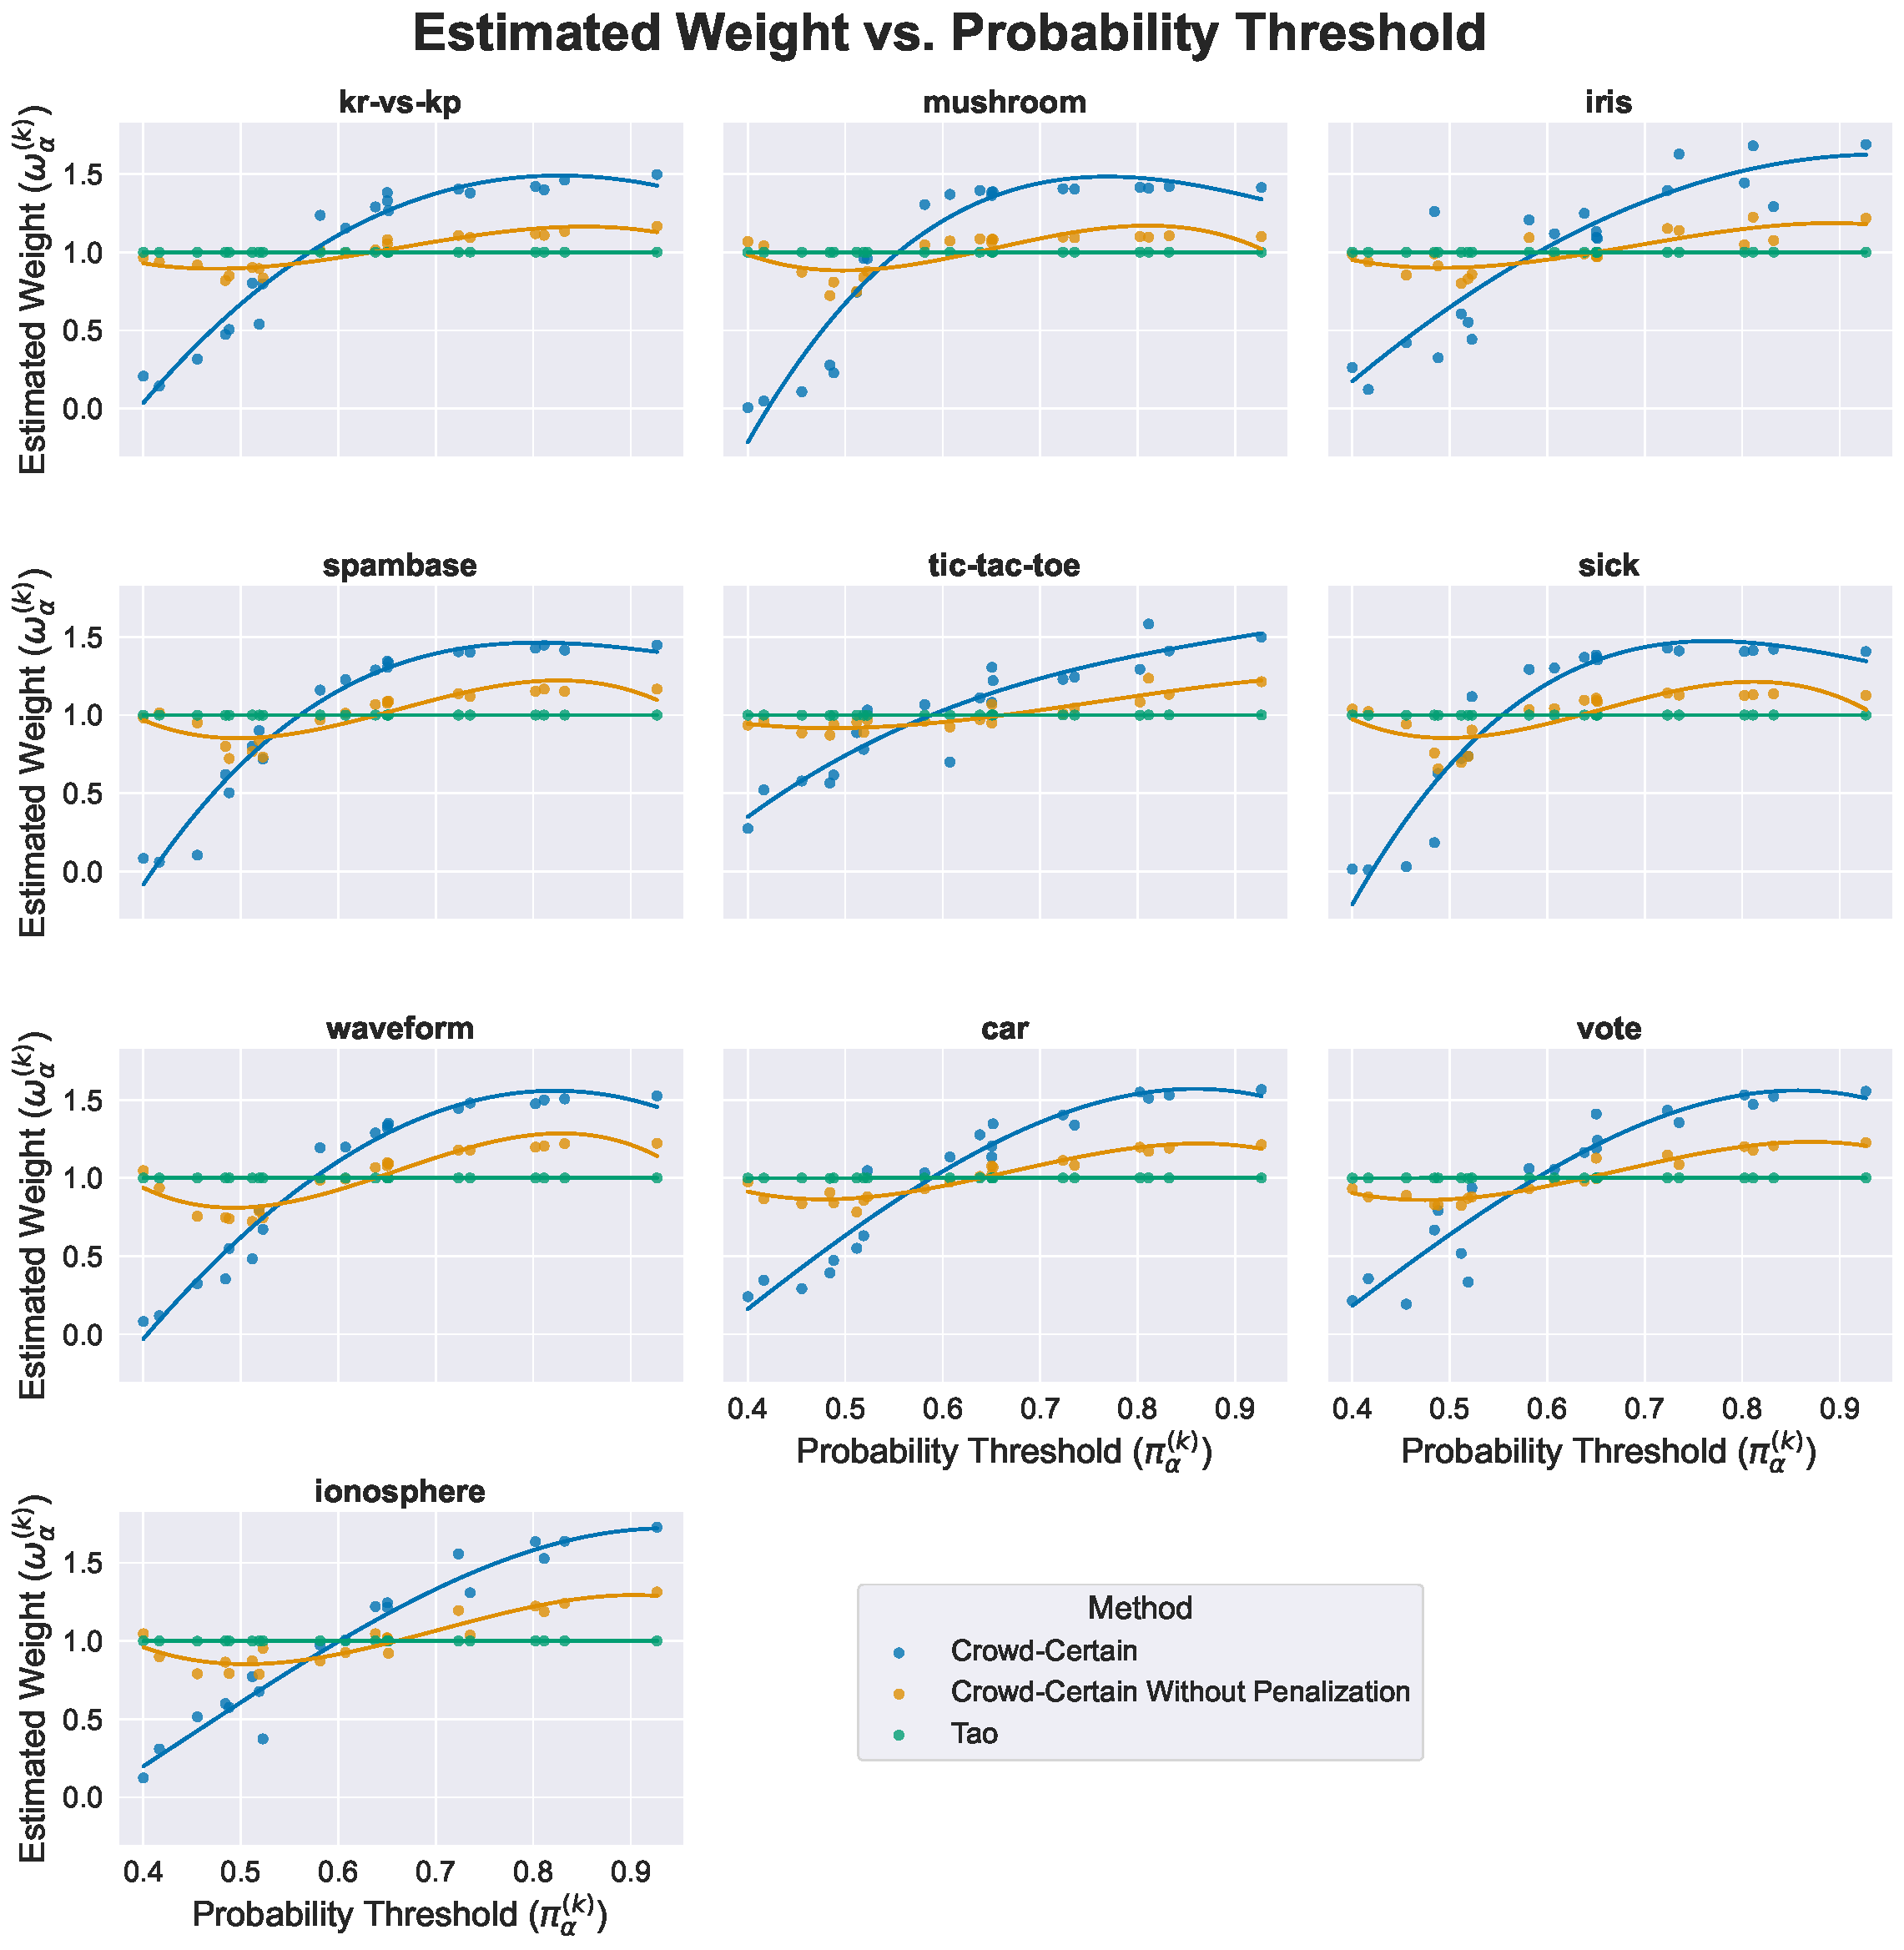
\includegraphics[width=\textwidth]{\figurepath{figure_weight_strength_relation/figure_weight_strength_relation.pdf}}
    \caption[Comparative Analysis of Weight Computation Techniques Across Ten Datasets]{A comprehensive comparison of weight computation techniques across ten distinctive datasets. Each subplot corresponds to a specific dataset, visually illustrating the relationship between the randomly assigned worker's probability threshold ($\pi_\alpha^{(k)}$) (represented on the horizontal axis) and the resulting computed weights ($\omega_{\alpha}^{(k)}$) (shown on the vertical axis). This relationship is analyzed for the Crowd-Certain method in two scenarios --- with and without penalization --- and is also compared with the Tao method~\cite{tao_Label_2020}. Individual data points represent real measured weights, while the overlaid curve delineates the corresponding regression line.}\label{fig:crowd.weight_strength_relation}
\end{figure}
\subsection{Label Aggregation Evaluation}
The Figure~\ref{fig:crowd.accuracy_per_worker} portrays the accuracy comparison of our label aggregation technique, termed Crowd-Certain, against ten existing methods, evaluated over ten distinct datasets. Each dataset was labeled by three different workers, with labels generated based on a uniform distribution and specific probability thresholds $\Pi_\alpha$ as explained in Section~\ref{subsec:methods.generating_fictitious_labelset}.
For a comprehensive evaluation, all experiments were repeated three times using different random seed numbers to account for randomness. The accuracy scores presented in the figure represent the average of these three runs and illustrate the degree of concordance between the aggregated label $\nu^{(i,k)}$ from each technique and the actual ground truth $y^{(i,k)}$.
It is important to note that, in the execution of our proposed technique, Crowd-Certain, the aggregated labels were derived through the application of the predicted probabilities, denoted as $\eta_{\alpha}^{(i,k)}$. This approach is significant as it enables the reuse of trained classifiers on future sample data, eliminating the need for recurrent simulation processes --- a substantial advantage in terms of computational efficiency. Conversely, the methodologies of existing techniques necessitated the use of actual crowd labels $z_\alpha^{(i,k)}$ to determine the aggregated labels. For example, in the case of Tao~\cite{tao_Label_2020} the aggregated labels were obtained using the following equation:
\begin{equation}
    \nu^{(i,k)} =
    \begin{cases}
        1 & \text{if } \left(\sum_{\alpha=1}^{M} \omega_{\alpha}^{(k)}\, z_{\alpha}^{(i,k)}\right) > 0.5 \\
        0 & \text{otherwise}
    \end{cases}
    \quad \forall i, k
    \label{eq:crowd.aggregated_label_benchmarks}
\end{equation}
These methods inherently involve re-running simulations for every new dataset, which could be computationally expensive and time-consuming. The Crowd-Certain method outperforms the existing methods, yielding higher average accuracy rates across 9 of the 10 evaluated datasets, while achieving a smaller accuracy compared to only one of the 10 benchmarks (MMSR) on tic-tac-toe dataset. For example, in the `kr-vs-kp' dataset, our proposed Crowd-Certain method achieved an average accuracy of approximately 0.923, significantly exceeding the highest-performing existing method that reached an accuracy of about 0.784. This trend holds true across other datasets as well, such as `mushroom', `spambase', and `waveform', where the Crowd-Certain method achieves superior average accuracies of around 0.98, 0.90, and 0.92, respectively.
\begin{figure}[htbp]
\centering
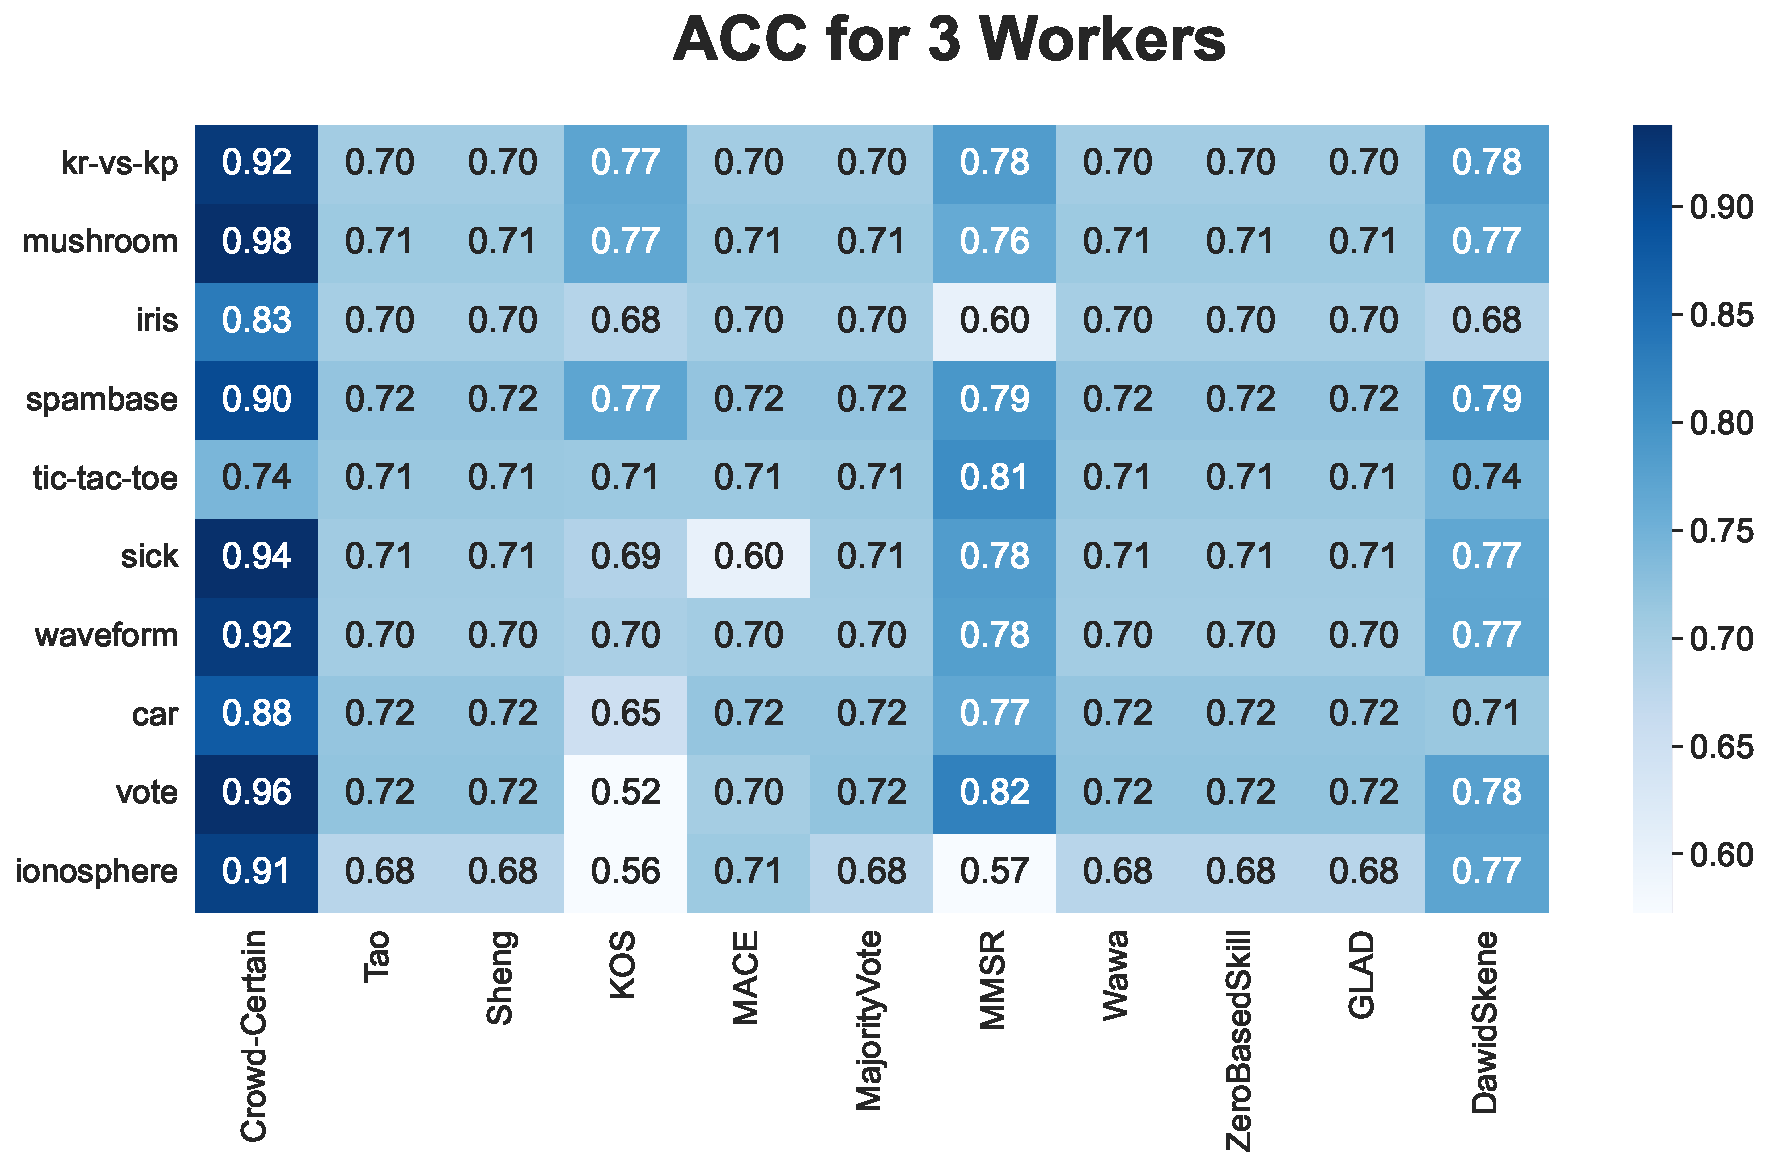
\includegraphics[width=\textwidth]{\figurepath{figure_metrics_mean_over_seeds_per_dataset_per_worker_ACC/figure_metrics_mean_over_seeds_per_dataset_per_worker_ACC.pdf}}
% \captionsetup{width=0.8\textwidth}
\caption[Comparison of Mean Accuracy for Crowd-Certain and Other Aggregation Methods with Three Crowd Workers.]{Comparative analysis of the mean accuracy between the proposed Crowd-Certain method and ten pre-existing label aggregation techniques, under conditions featuring three crowd workers. The depicted mean accuracy score is derived from an averaging process across three separate trials, each initiated with a distinct random seed, thus ensuring a fair and balanced comparison. Darker blue means higher mean accuracy.}\label{fig:crowd.accuracy_per_worker}
\end{figure}
We further extended our experiment to explore the effects of varying the number of workers, ranging from 3 up to 7. The results shown in Figure~\ref{fig:crowd.Fig.accuracy_all_datasets_workers} are presented as a series of box plots, each illustrating the distribution of accuracy (1st column), F1 (2nd column), and AUC (3rd column) scores across the 10 datasets for a given number of workers. These plots provide a visual summary of our technique's performance across various settings, including the median, quartiles, and potential outliers in the distribution of accuracies. Notably, our proposed Crowd-Certain technique shows improvements over the 10 benchmark methods for different number of workers. This enhancement is evident irrespective of the number of workers involved.
\begin{figure}[htbp]
    \centering
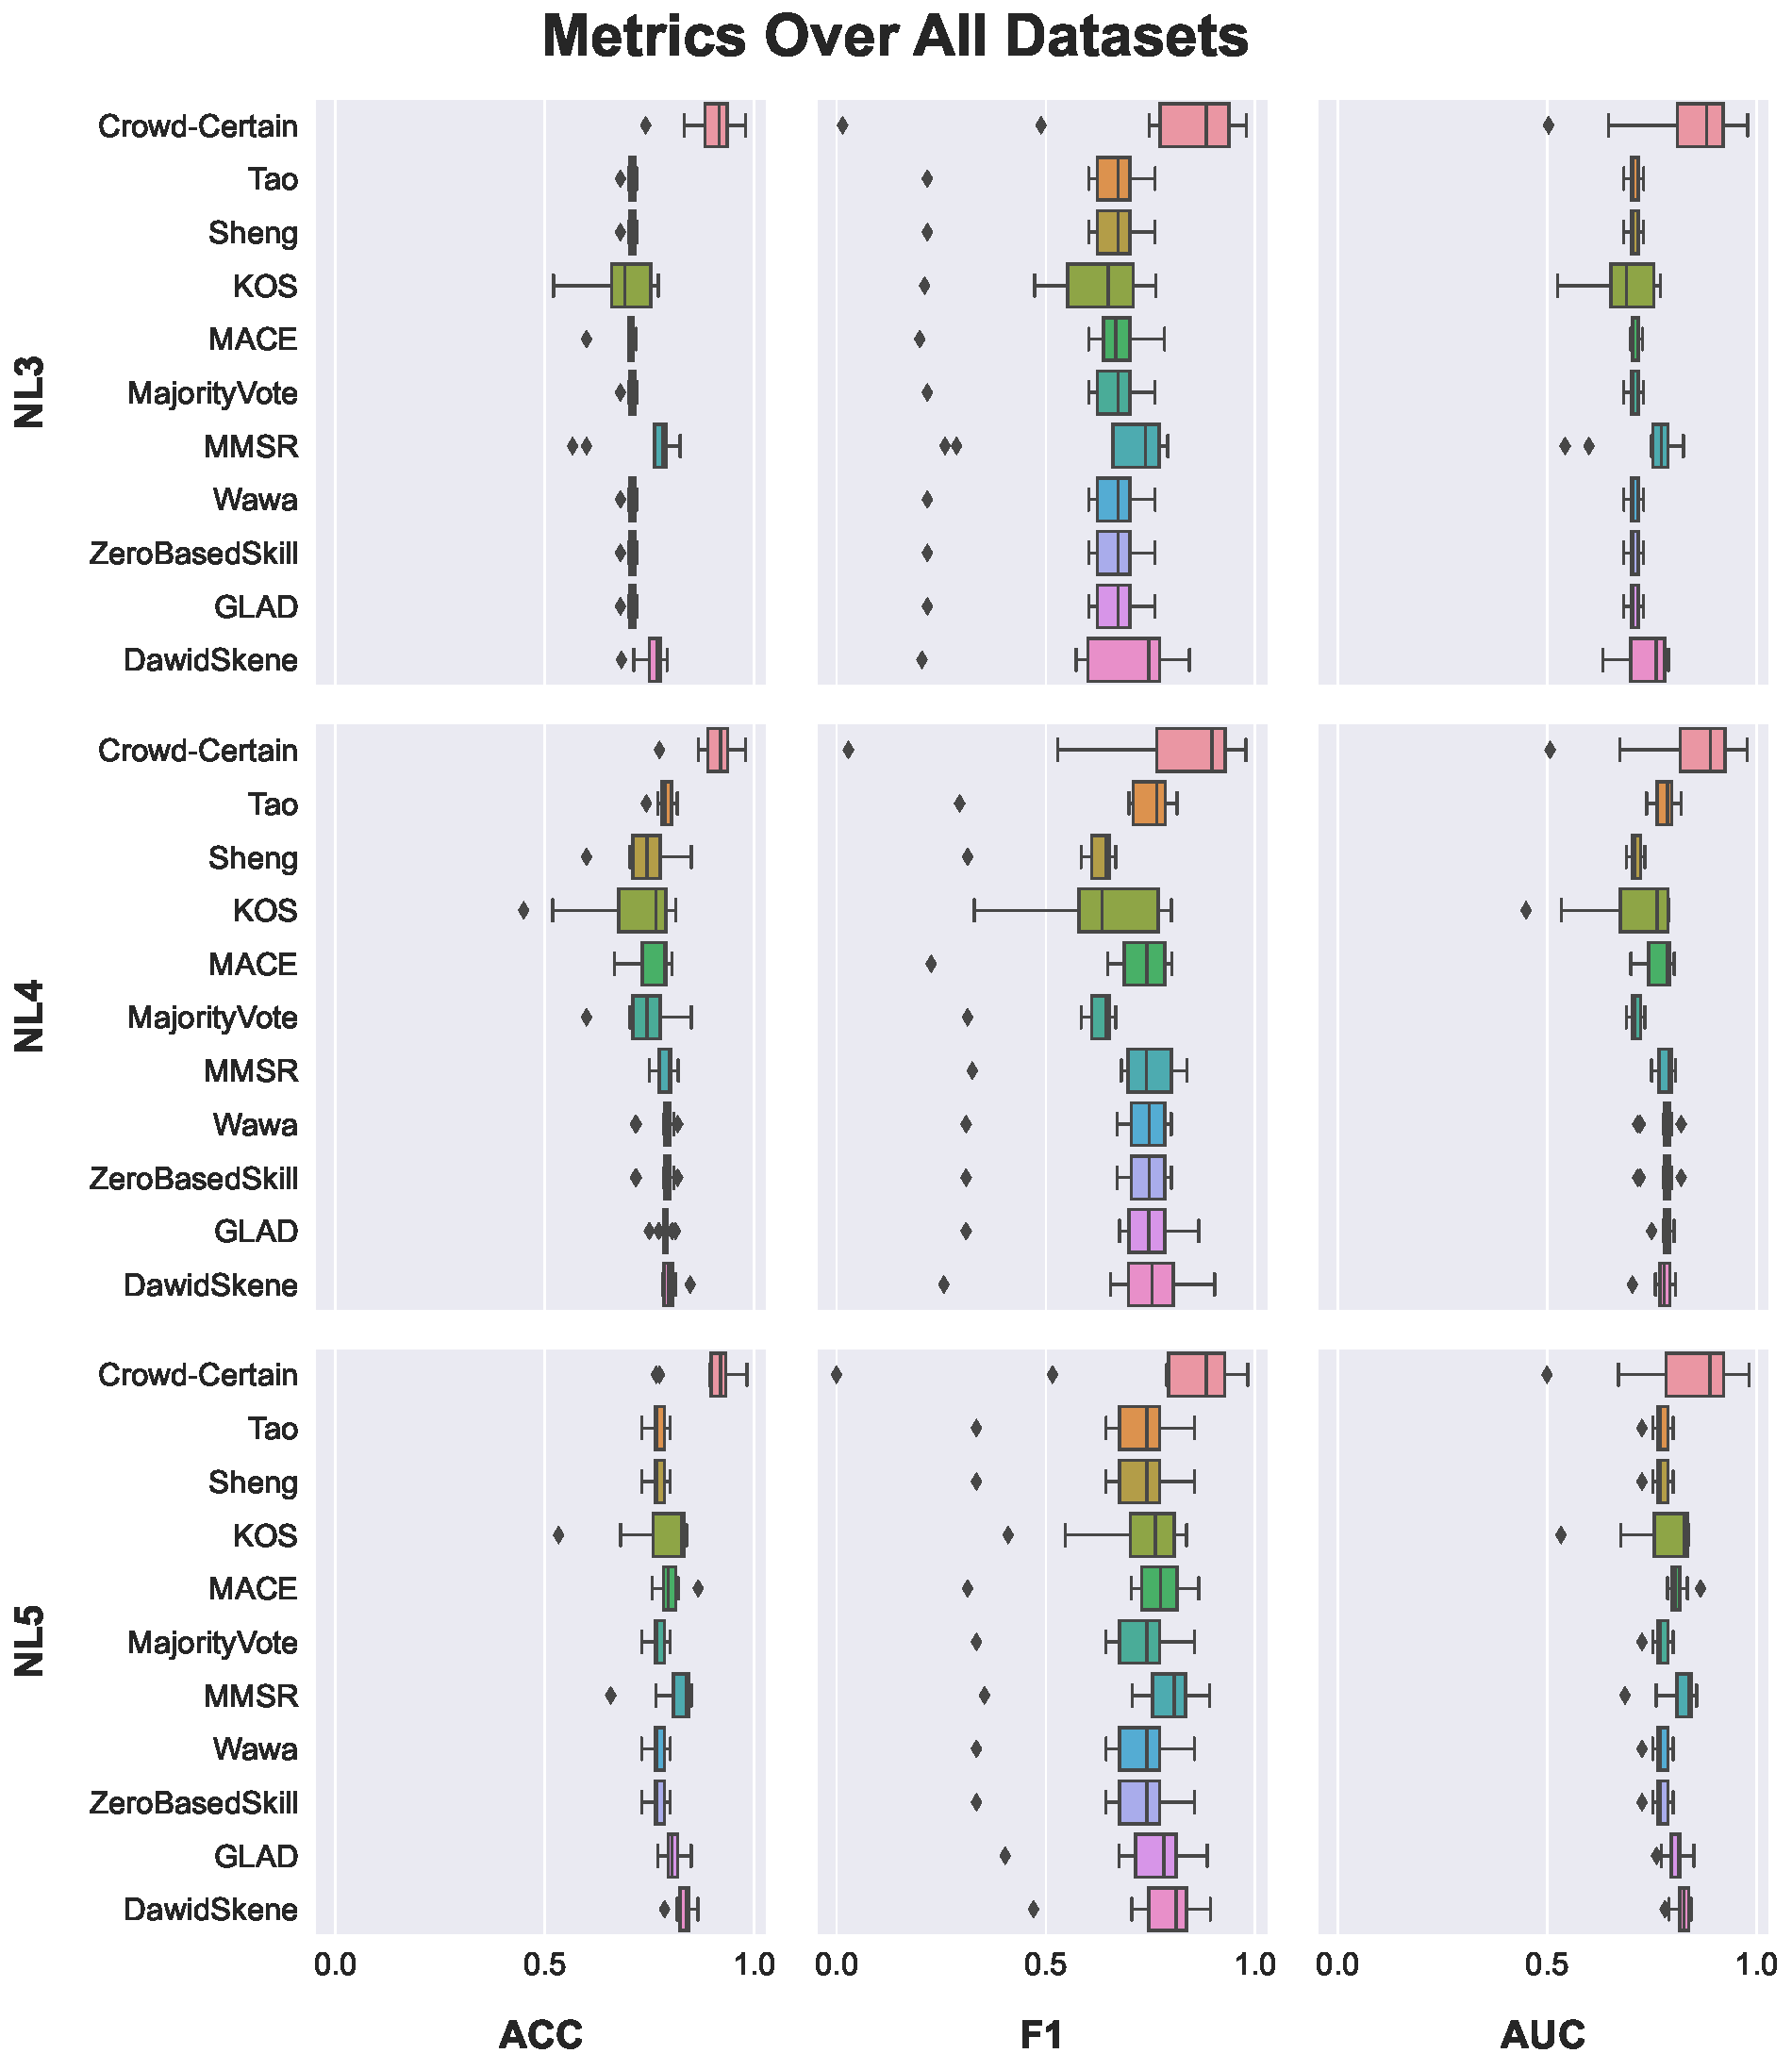
\includegraphics[width=\textwidth]{\figurepath{figure_metrics_all_datasets_workers/figure_metrics_all_datasets_workers.pdf}}%
    % \captionsetup{width=0.9\textwidth}
    \caption[Comparative Study of Accuracy, F1, and AUC Metrics for Label Aggregation Techniques Across Varied Crowd Sizes]  {This $3 \times 3$ structured figure provides a comprehensive comparison of Accuracy (first column), F1 (second column), and AUC scores (third column) across multiple label aggregation techniques (each shown with a unique color), including the proposed Crowd-Certain method and nine pre-existing techniques. Each row illustrates the results for a different number of crowd workers: the top row for three workers, the middle row for four workers, and the bottom row for five workers. Each subfigure presents ten boxplots, where each boxplot represents an aggregation technique. The metrics for each boxplot are computed from ten average scores, each corresponding to a distinct dataset. The average scores are derived from three independent trials, each with a different random seed. The aggregation of labels used in each experiment to calculate these metrics was obtained using Eq.~(\ref{eq:crowd.aggregated_label}) for Crowd-Certain and Eq.~(\ref{eq:crowd.aggregated_label_benchmarks}) for pre-existing techniques.}\label{fig:crowd.Fig.accuracy_all_datasets_workers}
\end{figure}
\subsection{Confidence Score Evaluation}
The Figure~\ref{fig:crowd.Fig.confidence_scores_all_datasets_3_workers} presents the evaluation of the two confidence score measurement techniques, namely Freq and Beta, using two performance metrics: Expected Calibration Error (ECE) and Brier Score. The evaluations were conducted across a variety of datasets and using three techniques: Crowd-Certain, Tao, and Sheng, when using three workers.
Figure~\ref{fig:crowd.Fig.confidence_scores_all_datasets_3_workers} depicts the performance of three different strategies: Crowd-Certain, Tao, and Sheng, compared across two metrics: ECE and Brier Score. These results are obtained using two different confidence score calculation techniques, Freq and Beta, applied over ten different datasets when three workers. The ECE offers an aggregated measure of the reliability of confidence scores ($F_{\Omega}^{(i,k)}$ and $F_{\beta}^{(i,k)}$) to assess the calibration of the aggregated labels across different techniques and strategies. A lower ECE indicates better-calibrated predictions, i.e., the estimated confidence scores are closer to the ground truth labels.\

Brier Score is a metric that quantifies the accuracy of probabilistic predictions. It calculates the mean squared difference between the estimated confidence scores ($F_{\Omega}^{(i,k)}$ and $F_{\beta}^{(i,k)}$) and the ground truth labels ($y^{(i,k)}$). Hence, higher Brier Score values correspond to better model performance. In Figure~\ref{fig:crowd.Fig.confidence_scores_all_datasets_3_workers}, it can be observed that for the Brier Score metric for both Beta ($F_{\beta}$) and Freq ($F_{\Omega}$) strategies, across all datasets, the proposed Crowd-Certain strategy consistently achieves higher scores when compared to Tao and Sheng. This indicates that the Crowd-Certain strategy offers better-calibrated predictions, providing a higher level of confidence in the aggregated labels.
For the ECE metric and Beta strategy ($F_{\beta}$) the Crowd-Certain strategy outperforms Tao and Sheng across most datasets. For the ECE metric and Freq strategy ($F_{\Omega}$), the Tao technique generally results in higher ECE, indicating worse calibration, whereas the Crowd-Certain and Sheng techniques show varying performance depending on the number of workers.
\begin{figure}[htbp]
    \centering
    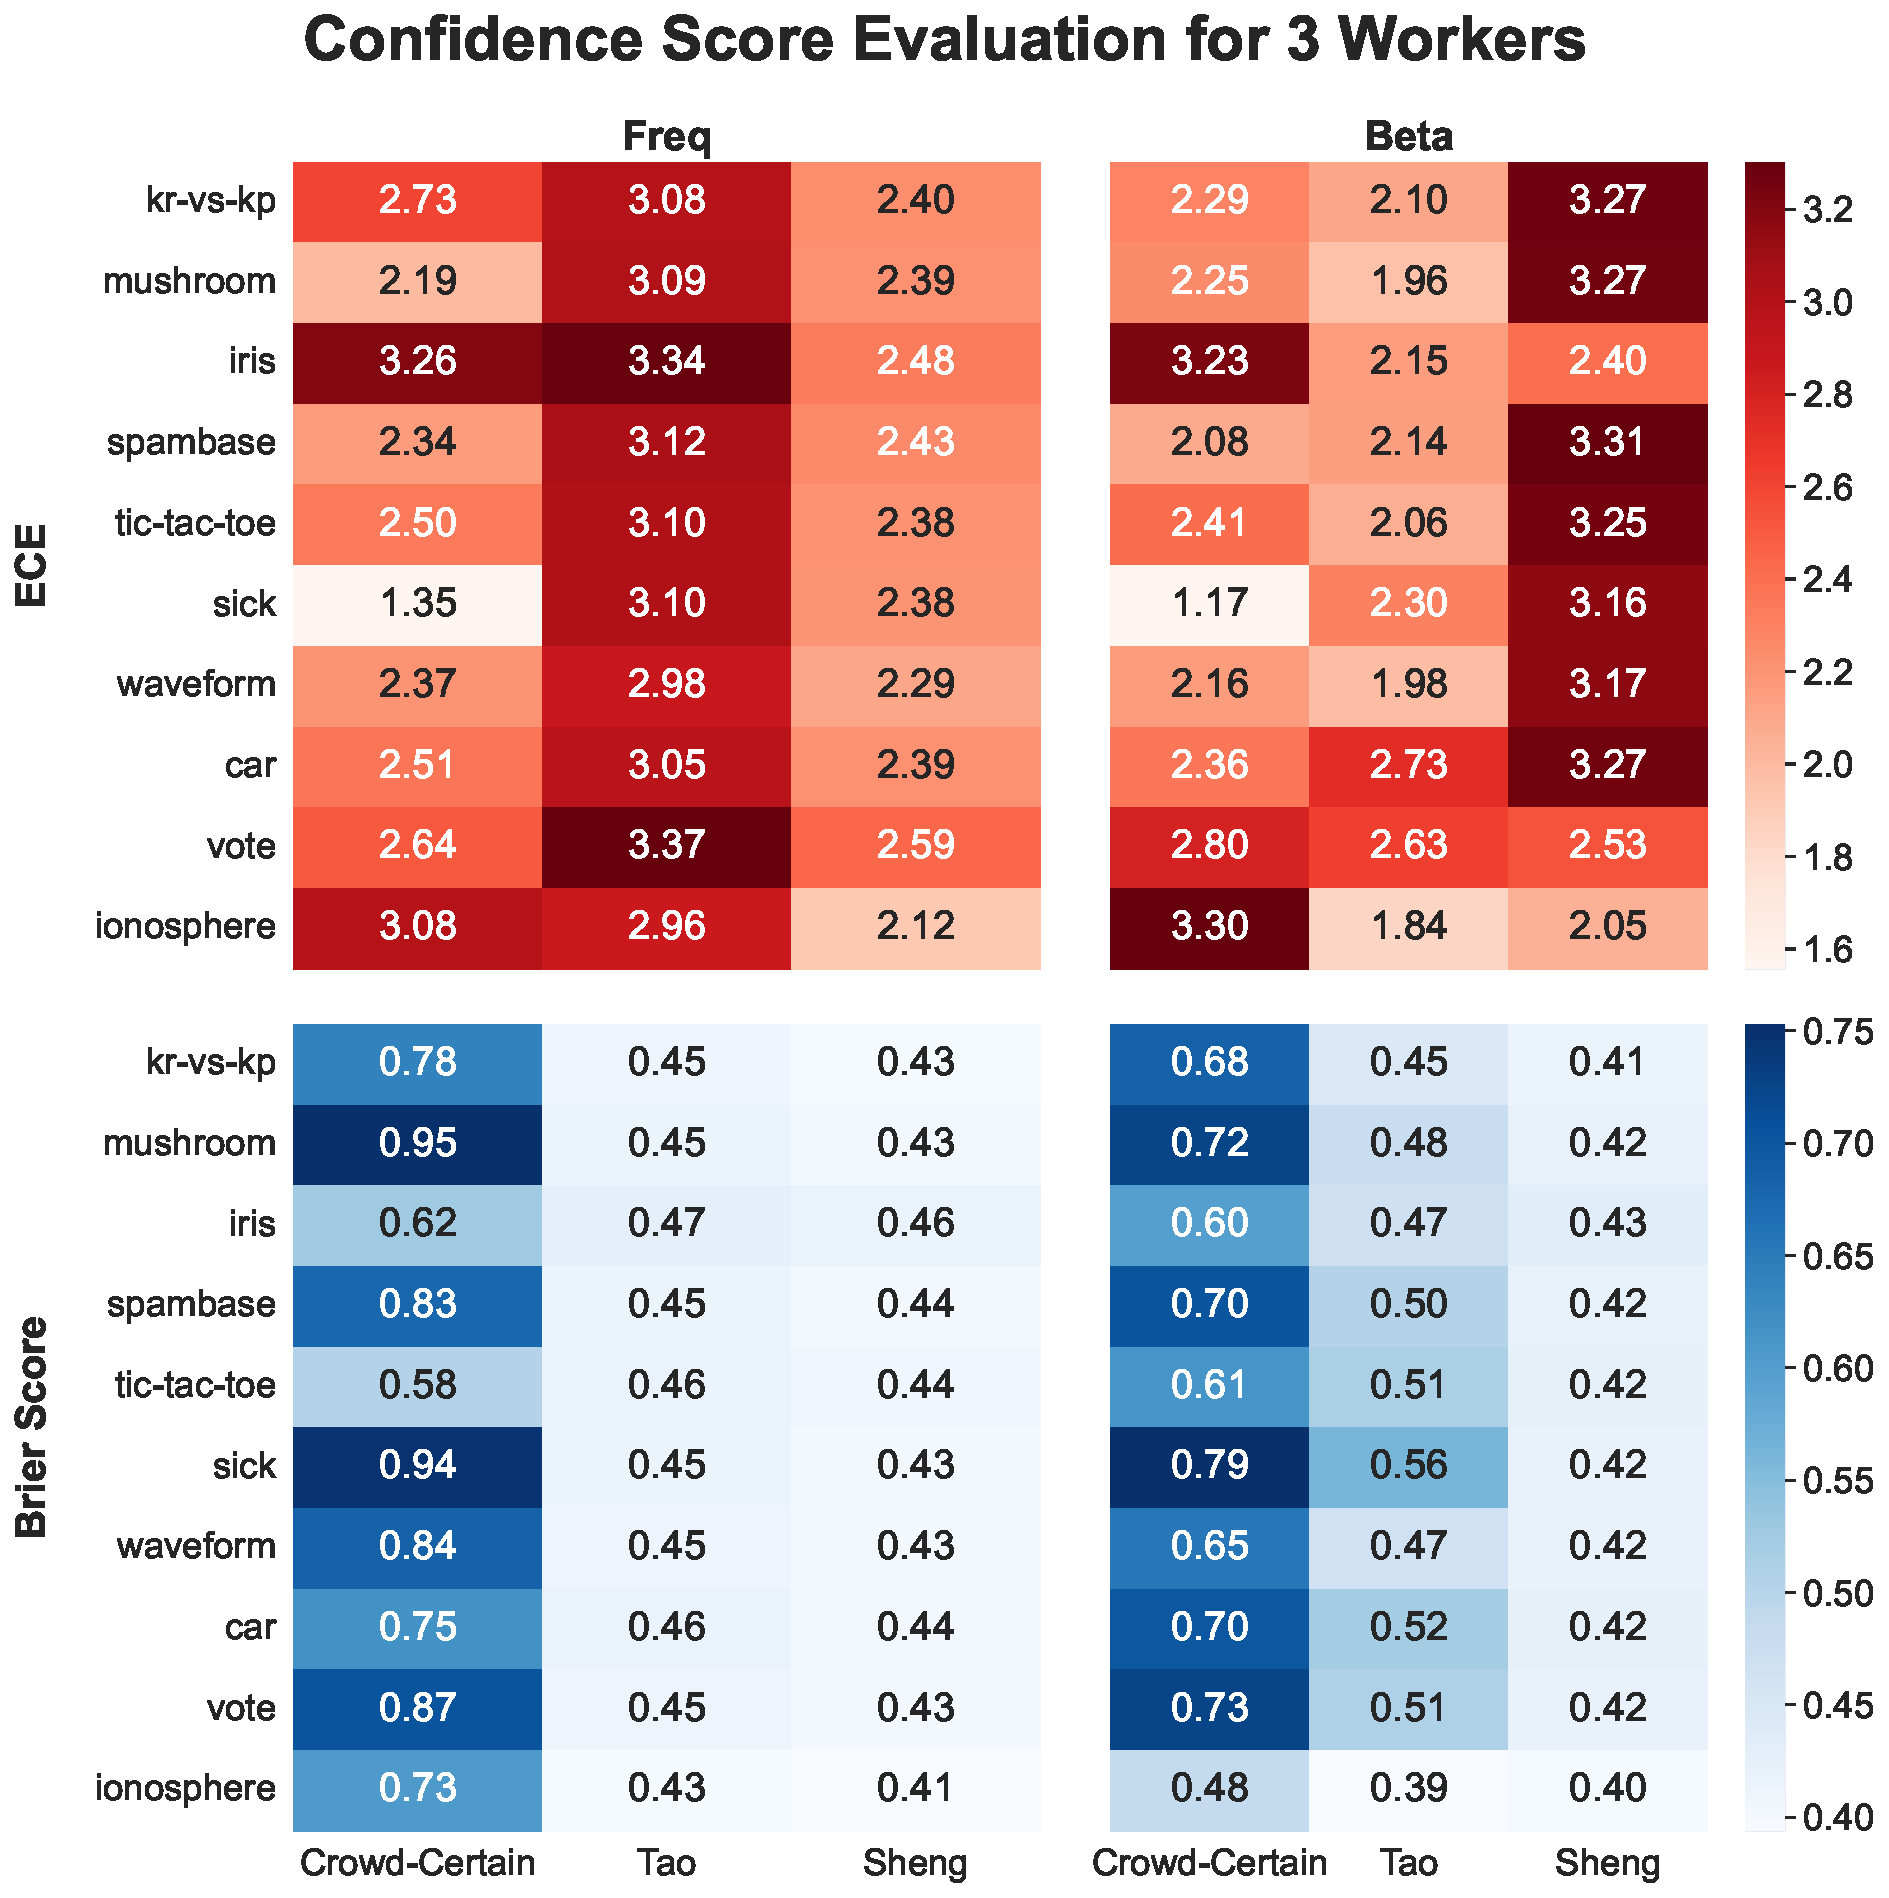
\includegraphics[width=\textwidth]{\figurepath{figure_heatmap_F_evals_all_datasets_NL3/figure_heatmap_F_evals_all_datasets_NL3.pdf}}
    % \captionsetup{width=0.8\textwidth}
    \caption[ECE and Brier Score Comparison across Techniques and Confidence Score Measurement Strategies for 3 Workers]{Comparative heatmap of the ECE and Brier Score across two confidence score measurement strategies: Beta ($F_{\beta}$) and Freq ($F_{\Omega}$). The comparison involves three different label aggregation techniques: Crowd-Certain, Tao, and Sheng, and spans ten distinct datasets for three crowd workers (NL3). The chosen metrics provide insight into the calibration of the predictions across different configurations}\label{fig:crowd.Fig.confidence_scores_all_datasets_3_workers}
\end{figure}
Figure~\ref{fig:crowd.Fig.confidence_score_one_datasets_all_workers} showcases the results for two metrics, ECE and Brier Score, for two confidence measurement techniques (Beta ($F_{\beta}$) and Freq ($F_{\Omega}$) strategies), applied using three different techniques: Crowd-Certain, Tao, and Sheng. These results are obtained for the kr-vs-kp dataset under different numbers of workers from 3 (denoted with NL3) up to (denoted with NL7). In general, the Brier Score decreases and ECE increases as the number of workers increases, which suggests that increasing the number of workers does not necessarily improve the performance. The performance varies depending on the confidence measurement technique and the strategy used. For the Freq strategy, the Crowd-Certain technique yields lower ECE and higher Brier Score across nearly all numbers of workers compared to the Tao and Sheng techniques, indicating more confident predictions when having only 3 workers. For the Beta strategy, the performance varies between techniques. For the Brier Score, the Freq strategy combined with the Crowd-Certain technique performs better across all numbers of workers compared to other combinations of techniques and strategies. For the ECE, the Beta strategy combined with the Crowd-Certain technique yields the lowest values for three and four workers, indicating a good match between predicted confidences and observed frequencies. However, the ECE generally exhibits a tendency to increase as the number of workers increases, indicating a decline in calibration.
\begin{figure}[htbp]
    \centering
    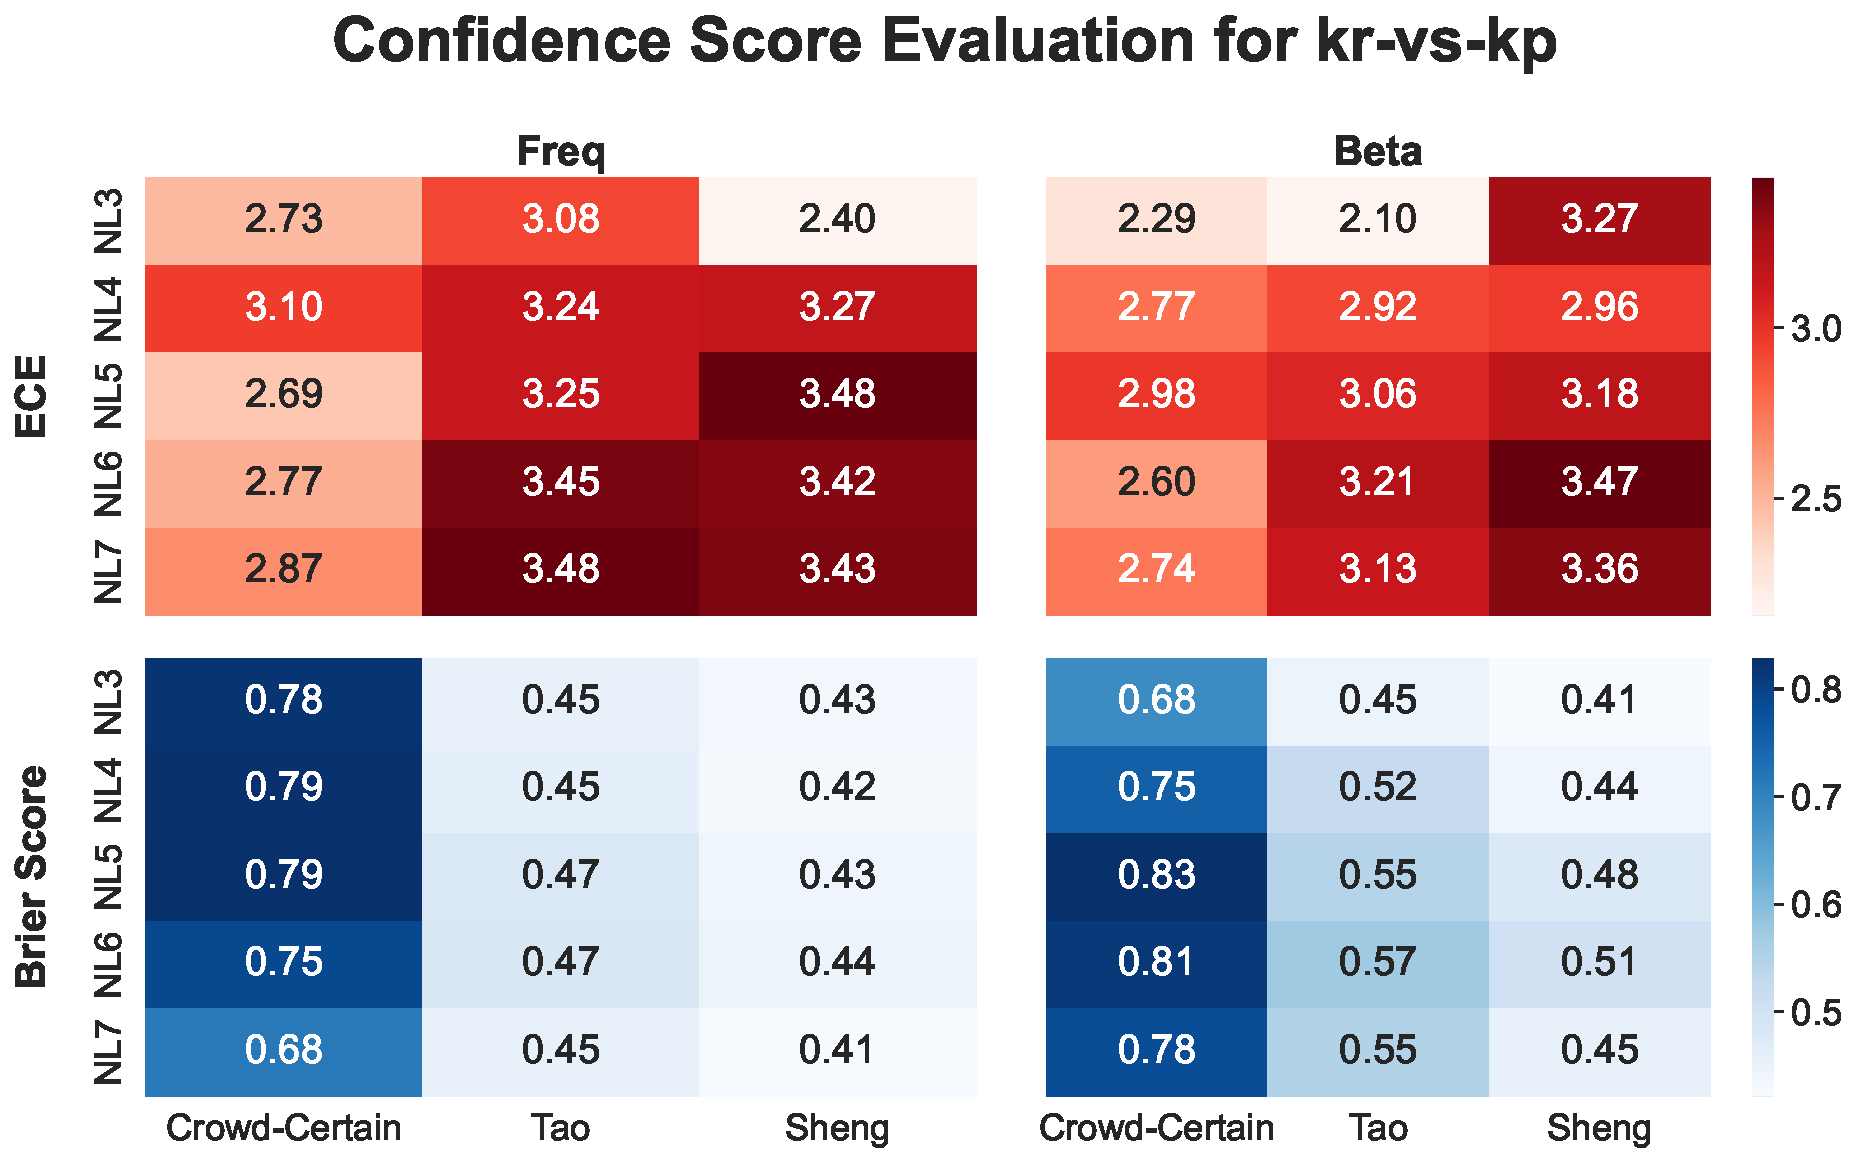
\includegraphics[width=\textwidth]{\figurepath{figure_heatmap_F_evals_kr-vs-kp_all_labelers/figure_heatmap_F_evals_kr-vs-kp_all_labelers.pdf}}
    % \captionsetup{width=0.8\textwidth}
    \caption[ECE and Brier Score Comparison across Techniques for Varying Number of Workers for kr-vs-kp Dataset] {Comparative evaluation of the ECE and the Brier Score across two confidence score measurement strategies: Beta ($F_{\beta}$) and Freq ($F_{\Omega}$). The results are plotted for three distinct label aggregation techniques --- Crowd-Certain, Tao, and Sheng --— on the kr-vs-kp dataset with varying numbers of crowd workers from three to seven (NL3 to NL7). }\label{fig:crowd.Fig.confidence_score_one_datasets_all_workers}
\end{figure}
Overall, these results suggest that the choice of the confidence measurement technique and the strategy have significant impacts on the calibration (confidence) of the predictions. Further investigations could be beneficial to understand the specific conditions under which certain techniques and strategies yield superior performance.
\section{Discussion}\label{sec:crowd.discussion}
Label aggregation is a critical component of crowdsourcing and ensemble learning strategies. Many generic label aggregation algorithms fall short because they do not account for the varying reliability of the workers. In this work, we introduced a new method for crowd labeling aggregation termed as Crowd-Certain. This technique effectively leverages uncertainty measurements to refine the aggregation of labels obtained from multiple workers. Through an extensive comparative analysis, it was shown to yield higher accuracy in label aggregation against ground truth, particularly in settings where only a limited number of workers are available. This advantage over established methods such as Gold Majority Vote, MV, MMSR, Wawa, Zero-Based Skill, GLAD, and Dawid Skene demonstrates the potential of the proposed method in enhancing the reliability of label aggregation in crowdsourcing and ensemble learning applications.
Our approach is distinguished by its application of a weighted soft majority voting scheme, where the weights are determined based on the level of uncertainty associated with each worker's labels. Importantly, the proposed technique takes into account the possibility of consistently inaccurate workers and includes measures to penalize them (shown in Eq.~\ref{eq:crowd.eq.10.consistency-penalized}), thus ensuring the credibility of the computed weights $\omega_{\alpha}^{(k)}$. The calculated weights follow a pre-set ground-truth accuracy closely, highlighting the effectiveness of the technique in capturing the quality of workers' labels. Moreover, the Crowd-Certain technique demonstrates an appreciable capability to generate confidence scores that accompany each aggregated label, offering an extended context that can be invaluable in practical applications.
In this study, we evaluated various techniques for aggregating crowdsourced labels and measuring the confidence scores associated with these labels. This evaluation involved two key metrics (ECE and Brier Score) for the evaluation of confidence scores, as well as three metrics (accuracy, AUC, and F1 score) for the evaluation of the aggregated labels ($\nu$). These metrics assessed different facets of model performance: calibration of the confidence scores (how confident the predictions are), and the performance of the aggregated labels against the ground truth. By comparison to existing methodologies, our method demonstrates superior performance across a variety of datasets, yielding higher average accuracy rates. Furthermore, our experiments, which involved varying the number of workers, demonstrated that Crowd-Certain outperforms the benchmark methods in nearly all scenarios, irrespective of the number of workers involved. This indicates that our approach is not only accurate and efficient, but also highly versatile to a range of settings, showing consistent improvements across different numbers of workers.
Significantly, our technique introduces an advantageous property by assigning a single weight ($\omega_{\alpha}^{(k)}$ for class $k$) to each worker $\alpha$ for all instances in the dataset. Moreover, the application of predicted probabilities ($\eta_{\alpha}^{(i,k)}$) in our method allows for the reuse of trained classifiers on future sample data, which eliminates the need for recurrent simulation processes. This presents a distinct advantage over conventional techniques, which require computationally expensive and time-consuming repeated simulations for every new dataset. It's worth noting that Crowd-Certain outperforms in nearly all evaluated scenarios across the tested datasets with one exception where the accuracy is lower than MMSR technique on tic-tac-toe dataset as shown in Figures~\ref{fig:crowd.accuracy_per_worker} and~\ref{fig:crowd.Fig.accuracy_all_datasets_workers}. This consistency is evident even when considering variance in dataset characteristics, such as `kr-vs-kp', `mushroom', and `spambase'.
In addition to label aggregation, the evaluation of confidence score measurements revealed further advantages of the Crowd-Certain method. When analyzing two confidence score measurement techniques, Freq and Beta, we found that our strategy achieves lower ECE scores compared to Tao and Sheng for most datasets. This implies that Crowd-Certain provides better-calibrated predictions, offering a higher level of confidence in the aggregated labels. Furthermore, Crowd-Certain also outperformed other techniques in terms of Brier Score across all datasets, indicating a higher accuracy of probabilistic predictions.
Our results indicate that the choice of aggregation and confidence measurement technique can significantly impact the performance. Furthermore, it shows that increasing the number of workers does not necessarily improve the performance, as indicated by the general increase in ECE and decrease (for Freq strategy) in Brier Score with a higher number of workers. This suggests a trade-off between the number of workers and the performance, and that the optimal number may depend on the specific context and the chosen techniques.
\section{Conclusion}\label{sec:crowd.conclusion}
The proposed Crowd-Certain label aggregation technique offers a promising solution for crowdsourced labeling tasks by providing a superior accuracy across various settings. Furthermore, it improves computational efficiency by allowing for the reuse of trained classifiers on future sample data, making it a viable option for large-scale data labeling tasks. While our findings are encouraging, further research and validation across more diverse datasets and real-world scenarios are warranted to further refine and enhance this approach. Future work could delve deeper into understanding why certain techniques and strategies outperform others under specific conditions. Further investigations could explore the effects of other factors such as the complexity of the task and the diversity of the crowd, which may impact the performance of different techniques and strategies. Our findings could guide future research and applications in this domain, with potential implications for various fields that rely on crowdsourced data, including machine learning, data science, and citizen science.
\section{Availability of Data and Materials}
The source code can be found at \href{https://github.com/artinmajdi/crowdcertain}{GitHub: @artinmajdi/crowdcertain}
% \section{Appendices}
% \section*{List of Abbreviations}
\section*{Competing Interests}
The authors declare that they have no competing interests.
% \section*{Acknowledgements}
\bibliographystyle{bst/sn-aps}
% \bibliographystyle{apalike}
\bibliography{subfiles/Better_BibTeX_Zotero.bib}
\end{document}

